% Full document code with \phantomsection workaround applied
\documentclass{book} % Or article, report - 'book' is good for longer combined documents

% Load packages
\usepackage{pdfpages} % For including PDF pages
\usepackage{hyperref} % Creates clickable links

% Hyperref setup
\hypersetup{
    colorlinks=true,
    linkcolor=blue,
    filecolor=magenta,
    urlcolor=cyan,
    pdftitle={415 Lecture Notes Combined},
    pdfpagemode=UseOutlines, % Show bookmarks panel
    bookmarksopen=true,      % Automatically open bookmarks panel
    bookmarksnumbered=true   % Number bookmarks like ToC entries
}

\begin{document}

% --- Add the overall title page ---
\title{415 Lecture Notes Combined}
\author{Gemini 2.5 Pro} % Adjust author if needed
\date{May, 2025} % Adjust date if needed
\maketitle

% --- Add a Table of Contents ---
% This will list the "Lecture #" entries we add below.
\tableofcontents

\cleardoublepage % Start included PDFs on a right-hand page (for book class)
                  % Use \newpage if using article class

% --- Include the PDFs with ToC entries, including ALL pages ---
% The 'pages=-' command includes all pages from each PDF.
% The '\phantomsection' provides an anchor for hyperref.
% The '\addcontentsline{toc}{chapter}{Lecture X}' adds an entry to the ToC pointing to the phantomsection anchor.
% Removed 'linktodoc=true' from \includepdf as we are manually creating anchors.

% Include files 1 through 16
\phantomsection
\addcontentsline{toc}{chapter}{Lecture 1}
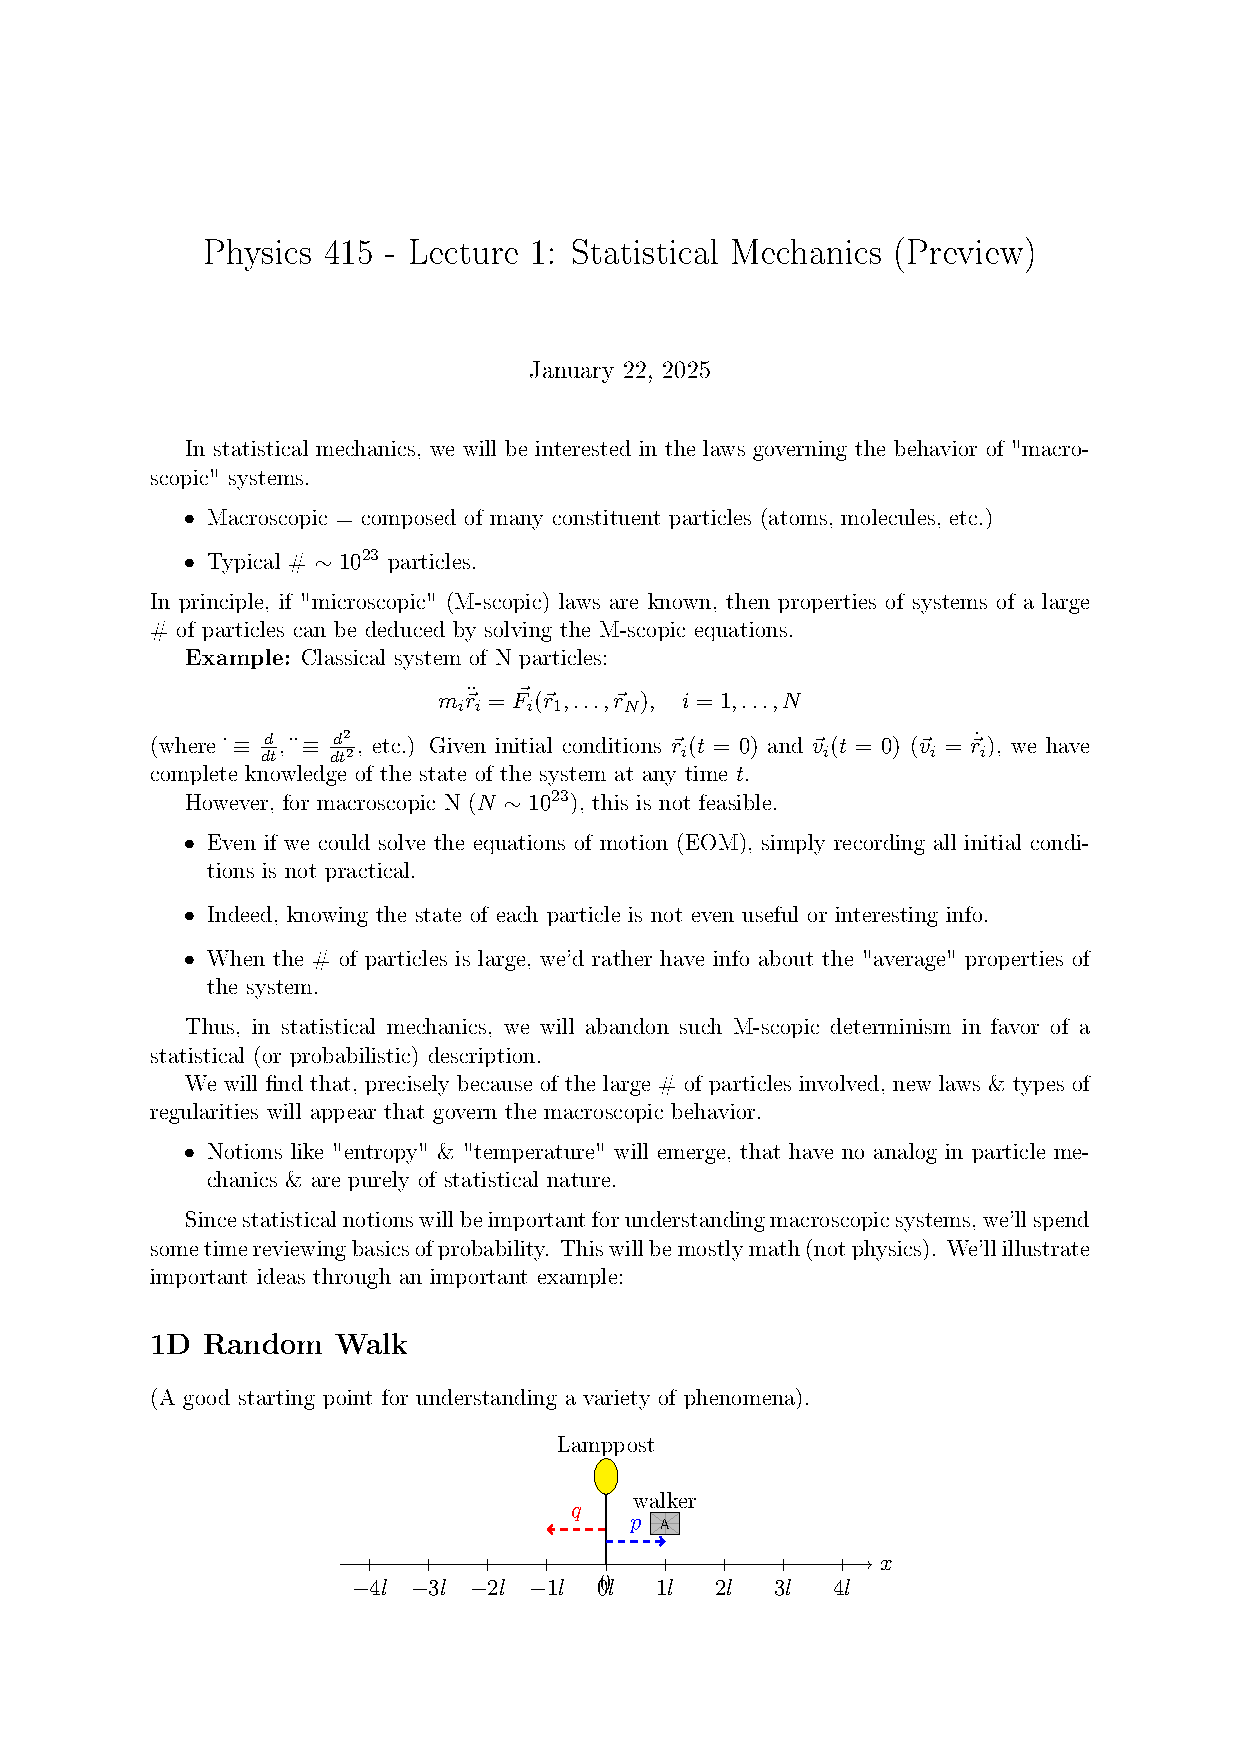
\includepdf[pages=-]{1.pdf}
\cleardoublepage % Added for consistency between chapters
\phantomsection
\addcontentsline{toc}{chapter}{Lecture 2}
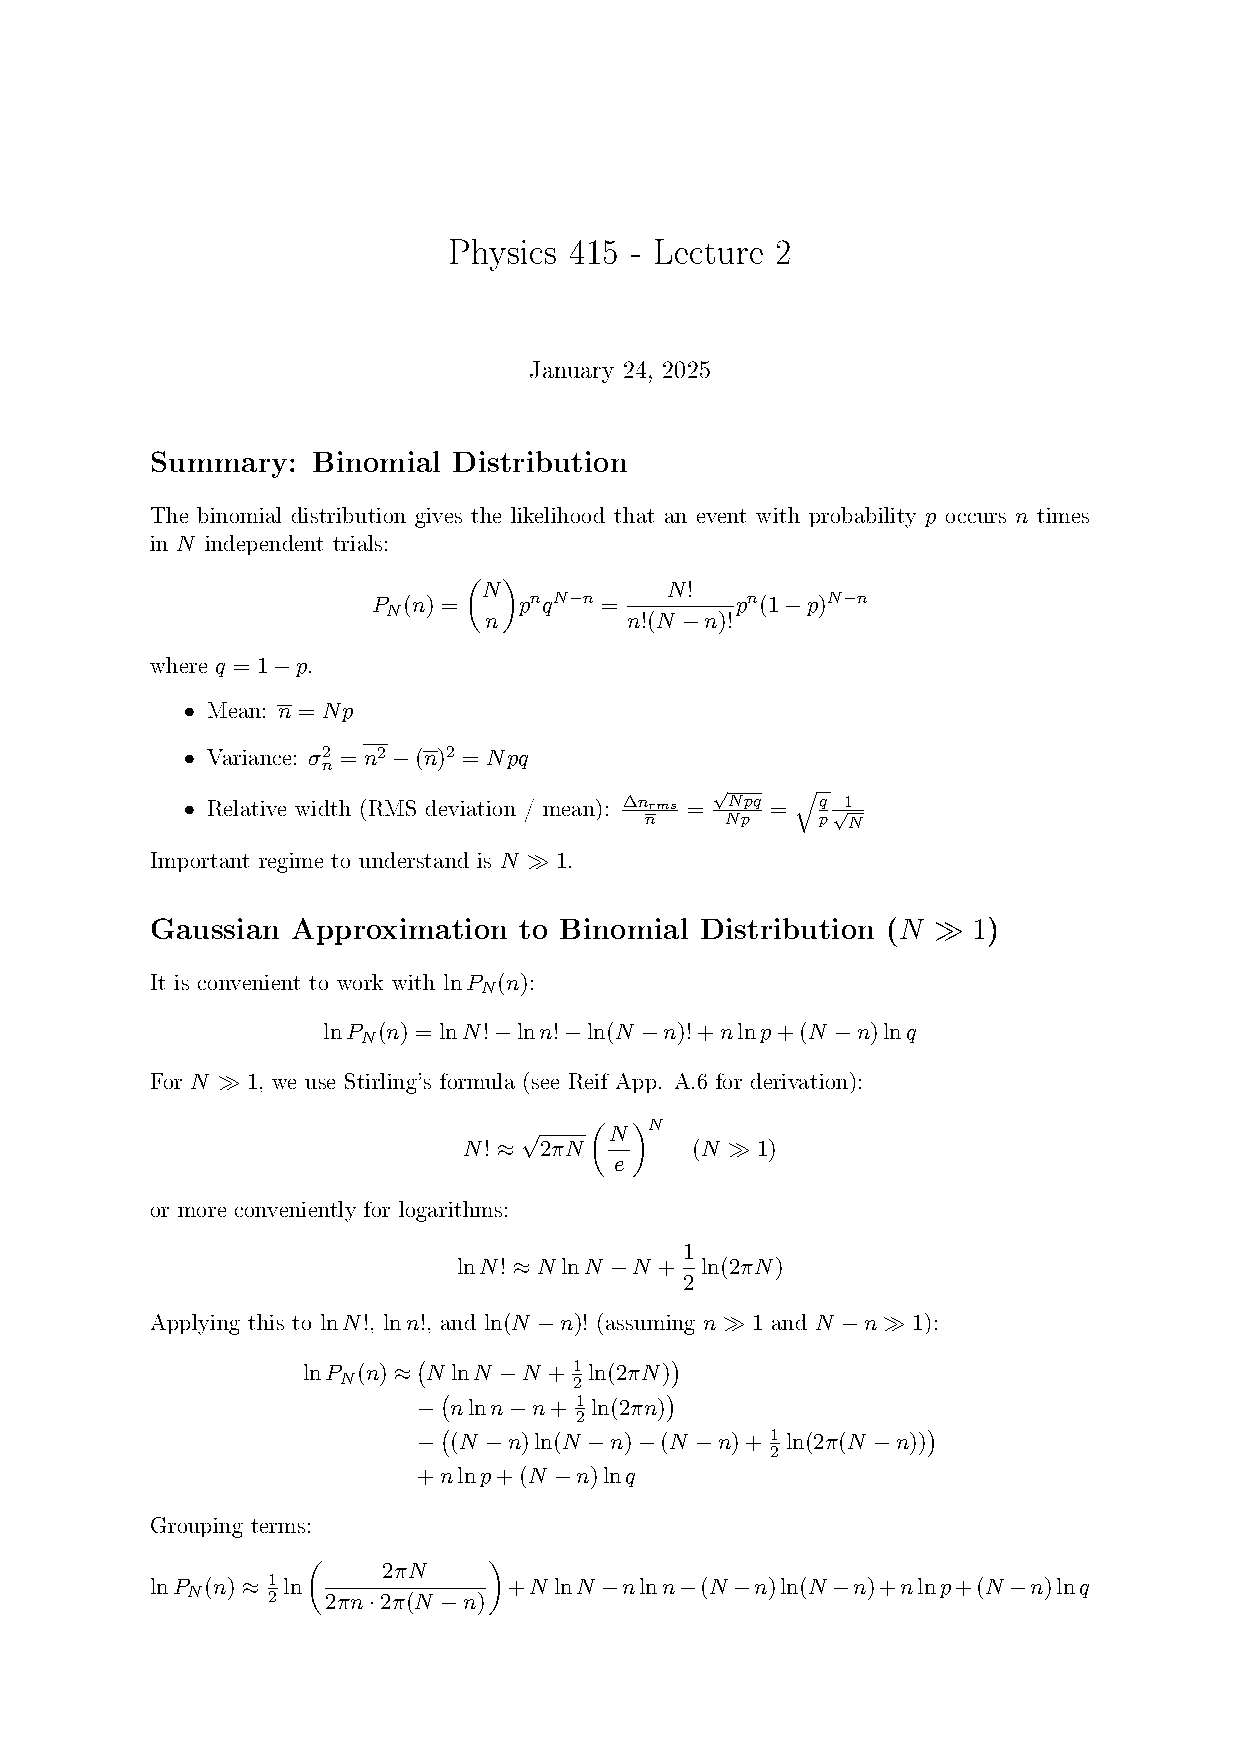
\includepdf[pages=-]{2.pdf}
\cleardoublepage
\phantomsection
\addcontentsline{toc}{chapter}{Lecture 3}
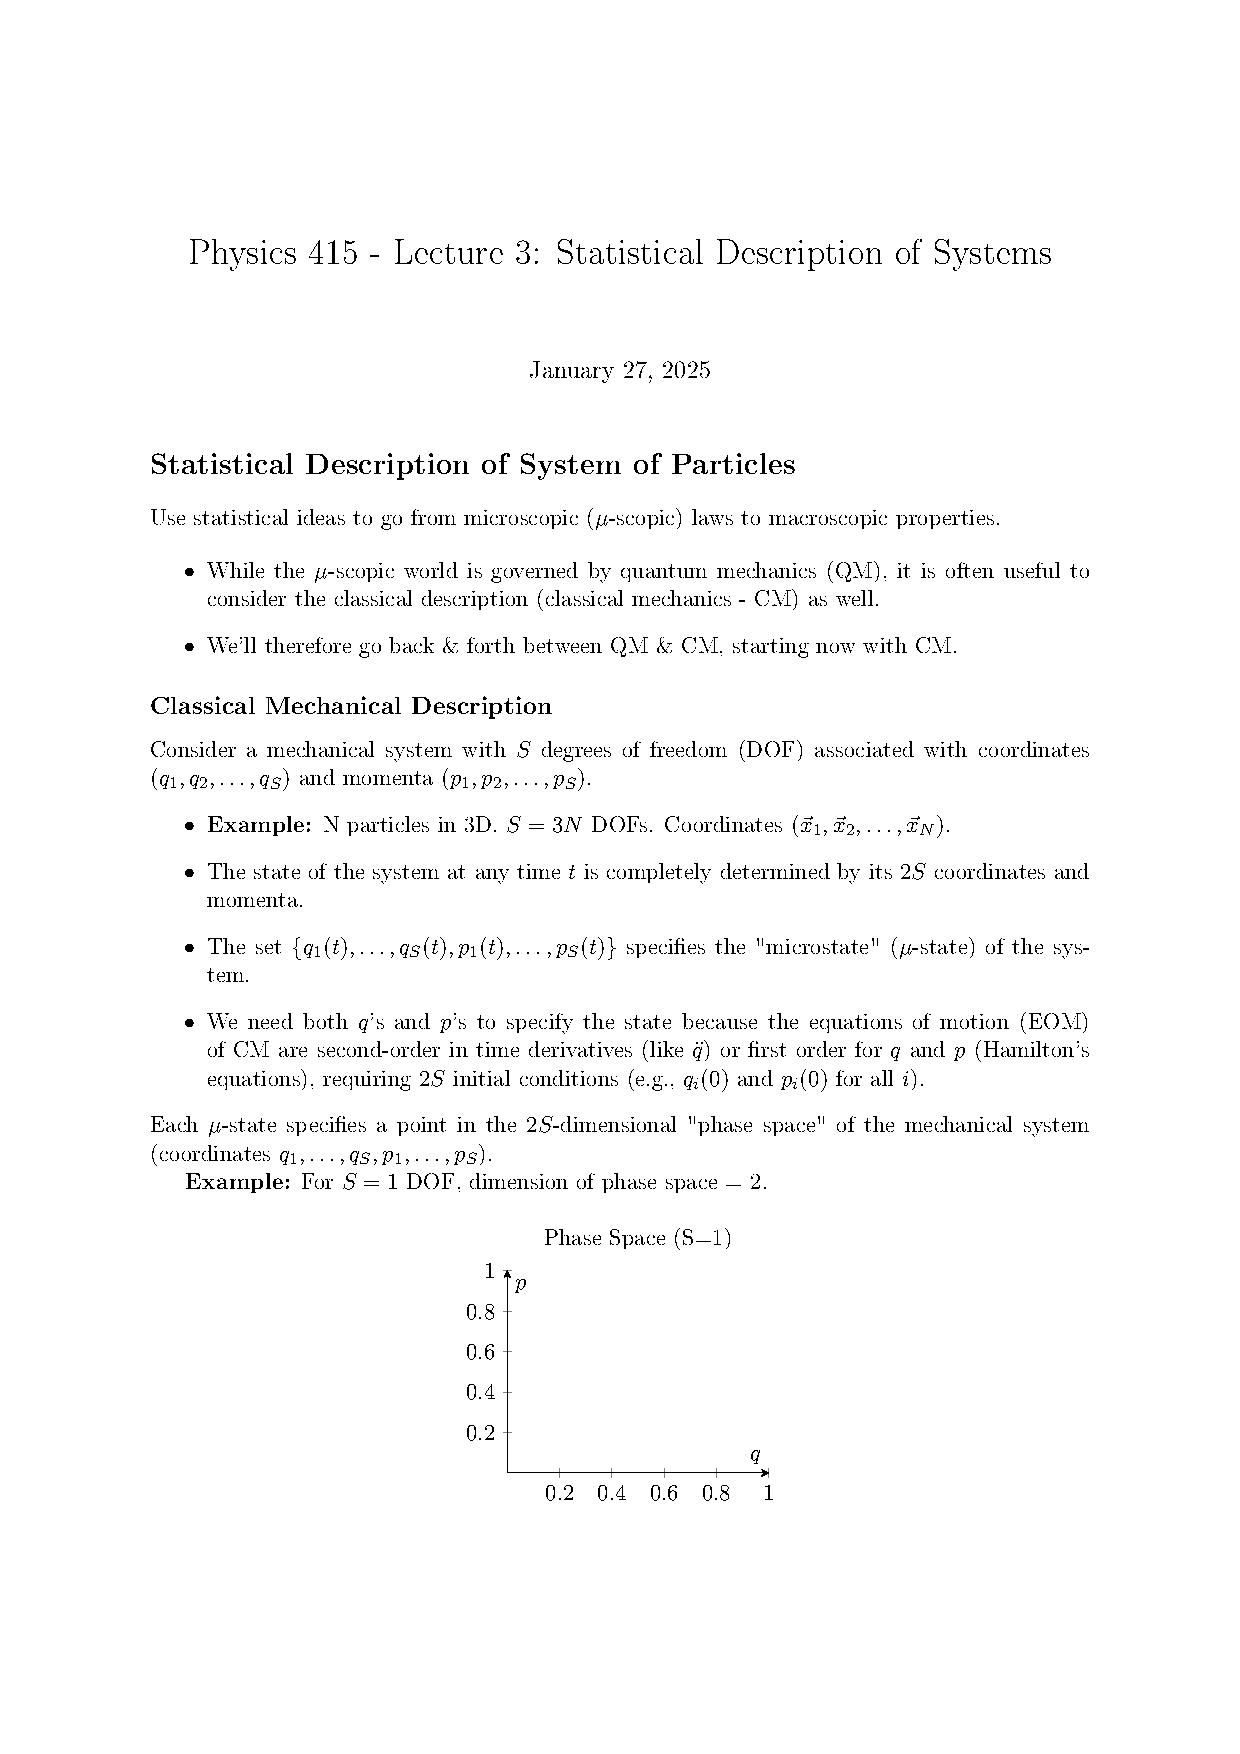
\includepdf[pages=-]{3.pdf}
\cleardoublepage
\phantomsection
\addcontentsline{toc}{chapter}{Lecture 4}
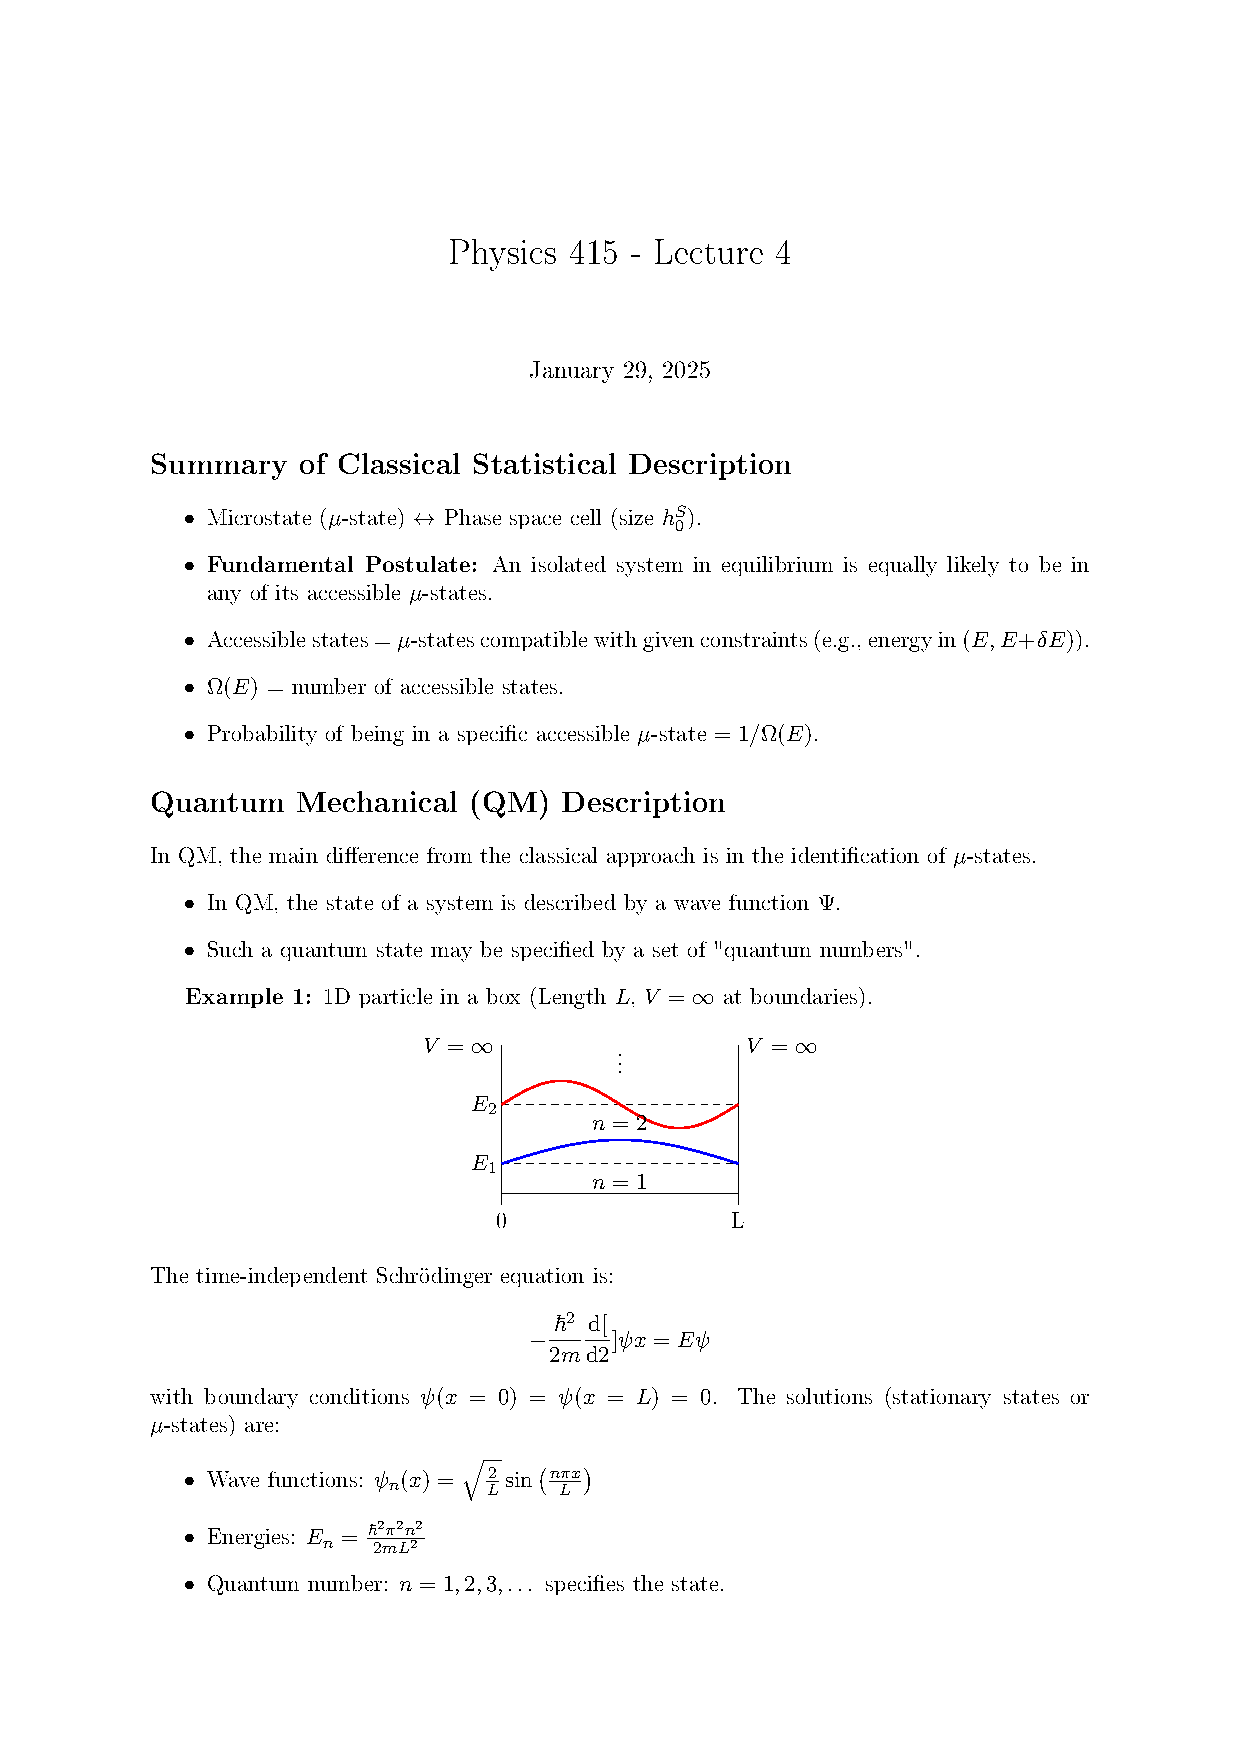
\includepdf[pages=-]{4.pdf}
\cleardoublepage
\phantomsection
\addcontentsline{toc}{chapter}{Lecture 5}
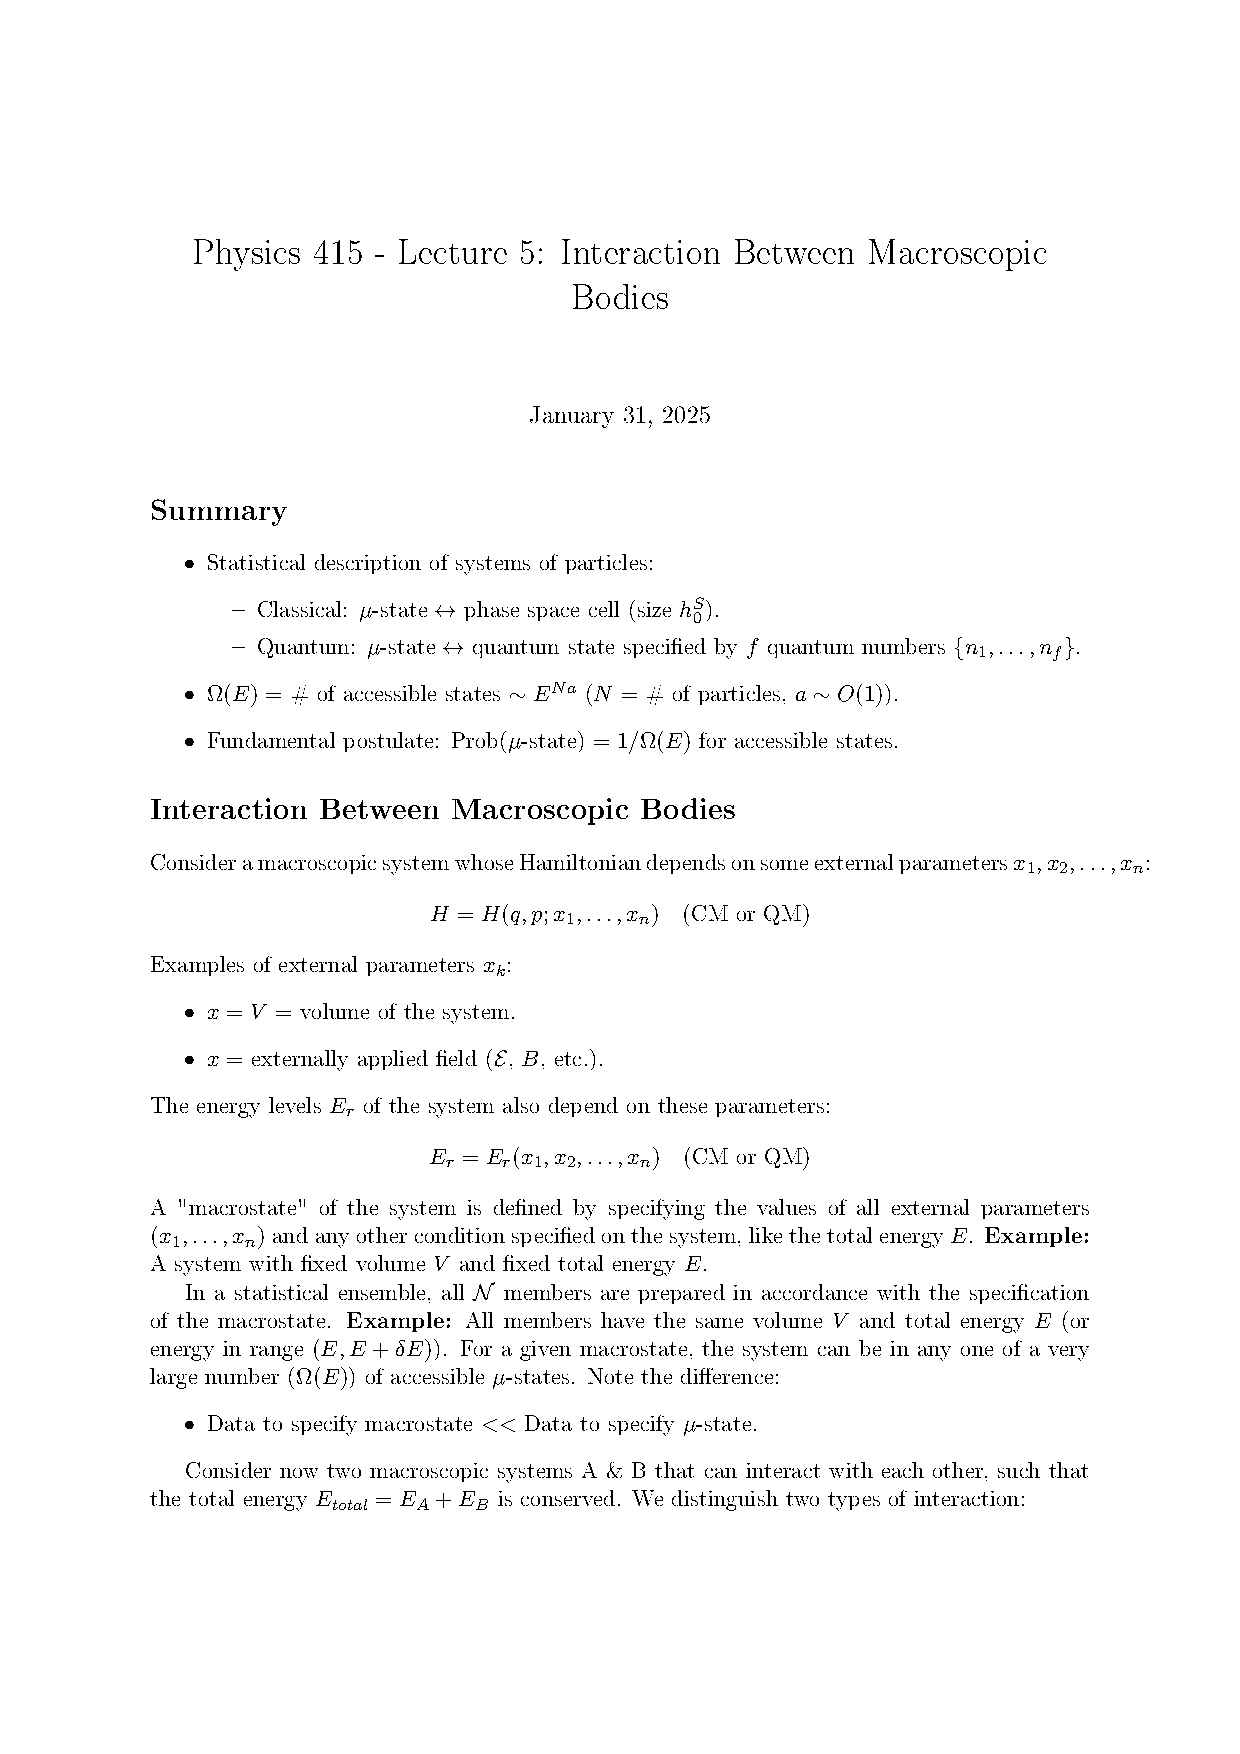
\includepdf[pages=-]{5.pdf}
\cleardoublepage
\phantomsection
\addcontentsline{toc}{chapter}{Lecture 6}
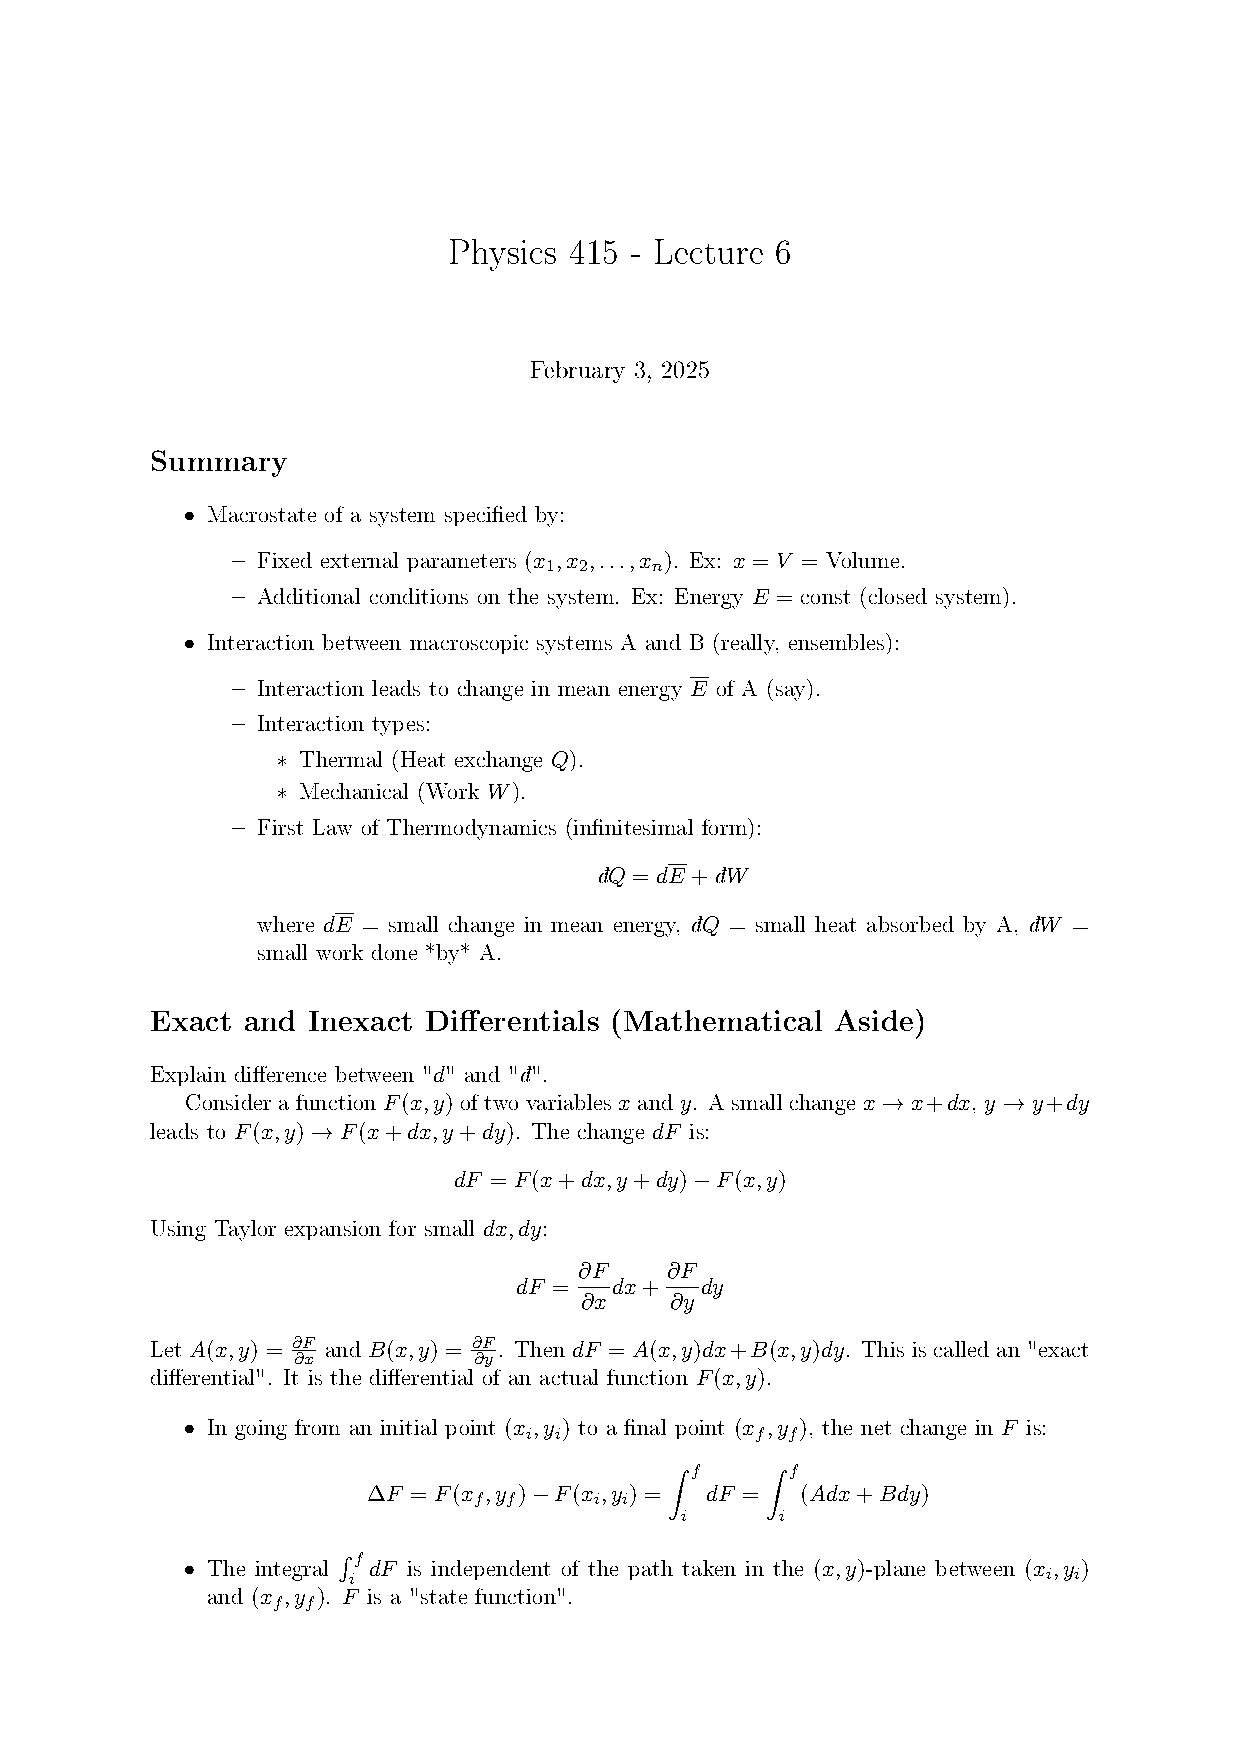
\includepdf[pages=-]{6.pdf}
\cleardoublepage
\phantomsection
\addcontentsline{toc}{chapter}{Lecture 7}
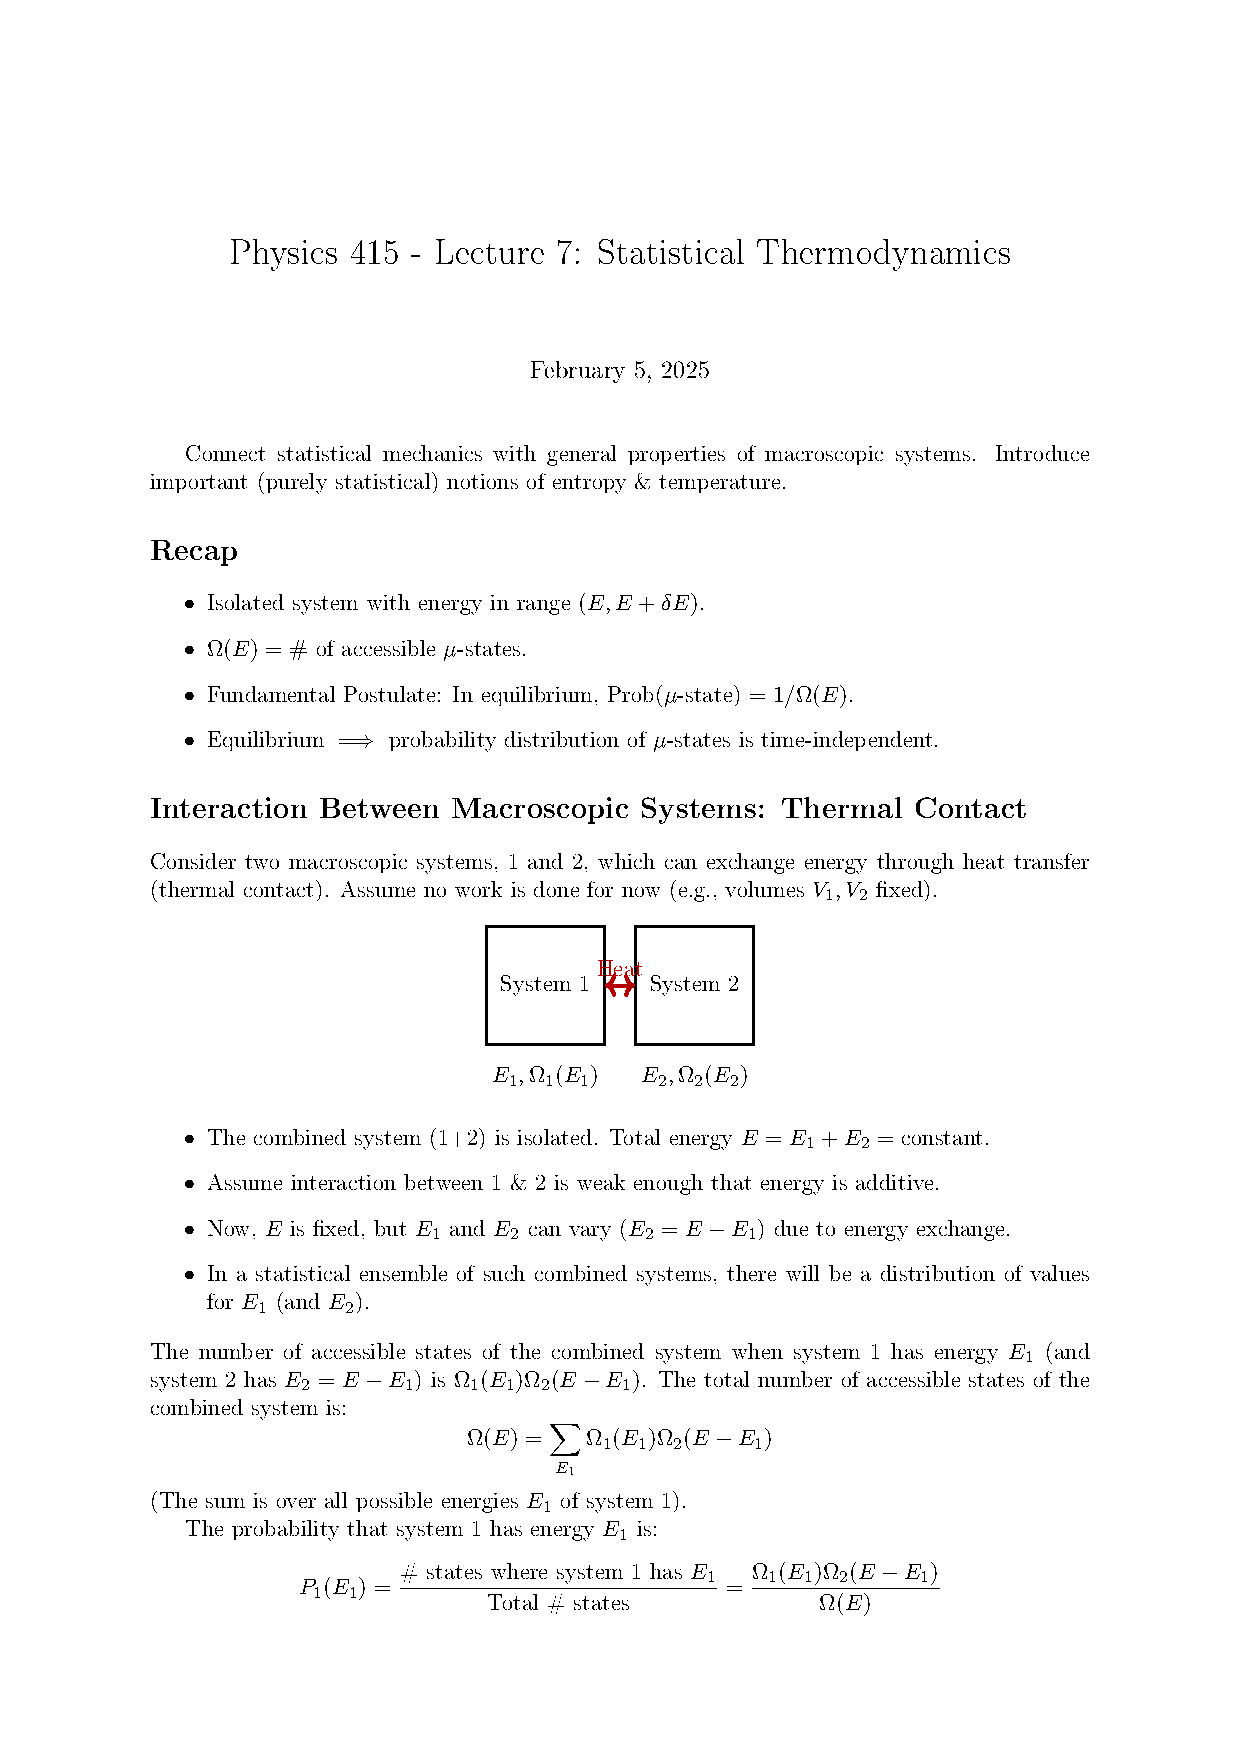
\includepdf[pages=-]{7.pdf}
\cleardoublepage
\phantomsection
\addcontentsline{toc}{chapter}{Lecture 8}
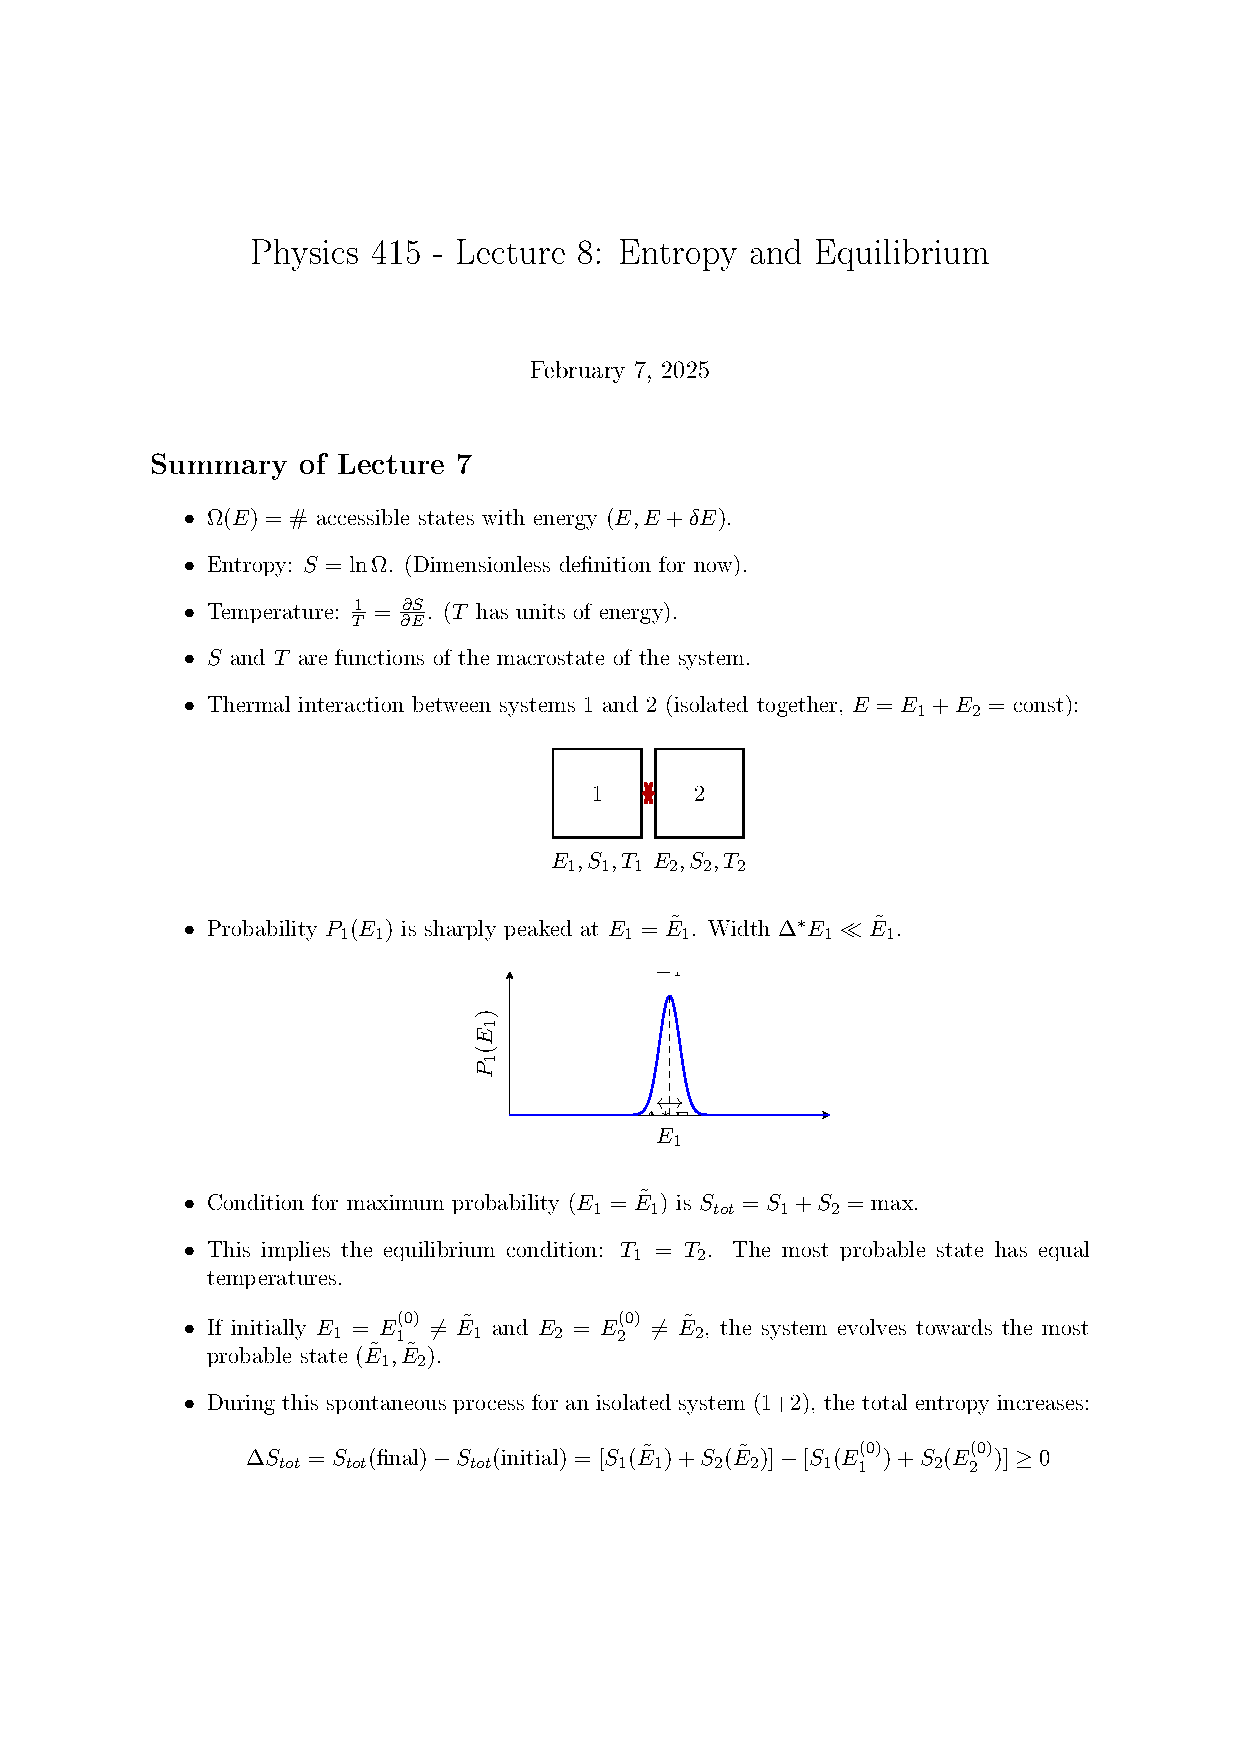
\includepdf[pages=-]{8.pdf}
\cleardoublepage
\phantomsection
\addcontentsline{toc}{chapter}{Lecture 9}
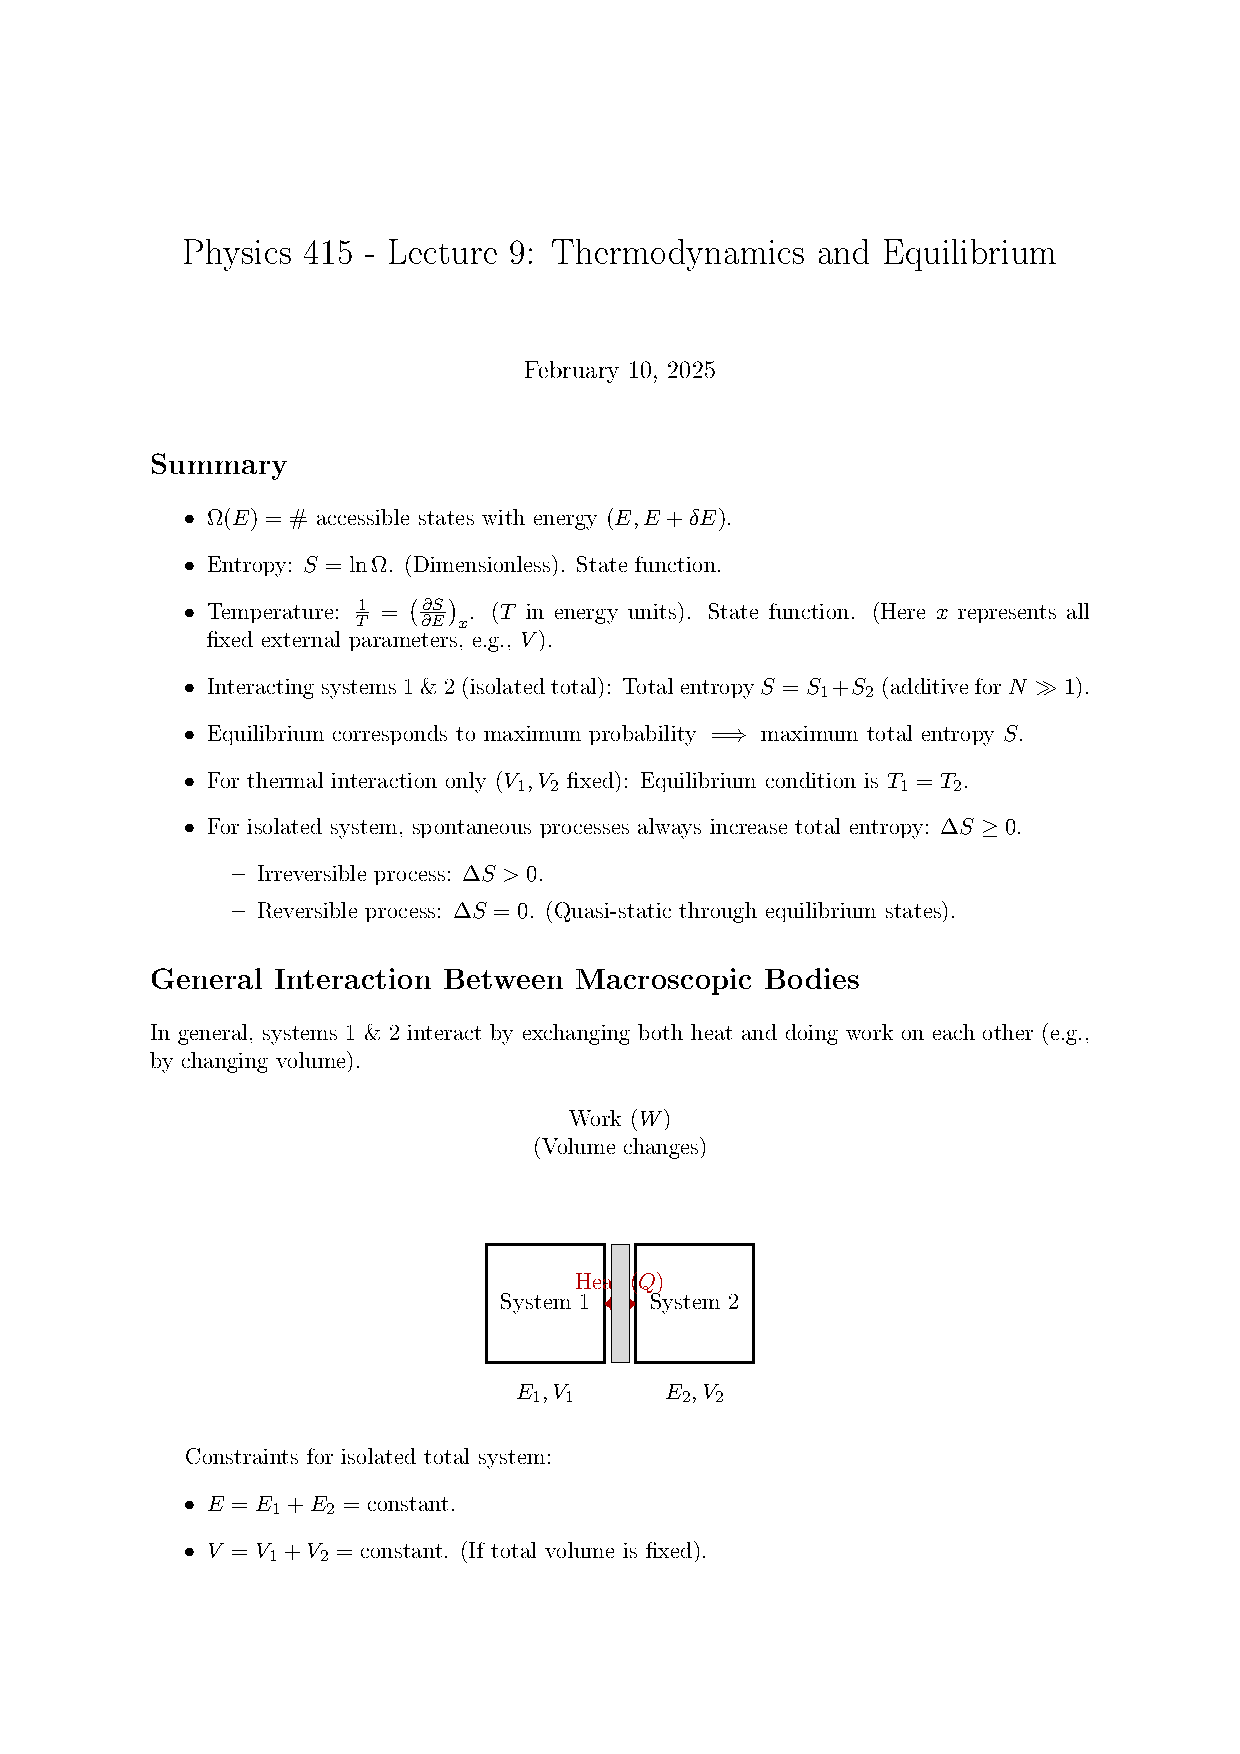
\includepdf[pages=-]{9.pdf}
\cleardoublepage
\phantomsection
\addcontentsline{toc}{chapter}{Lecture 10}
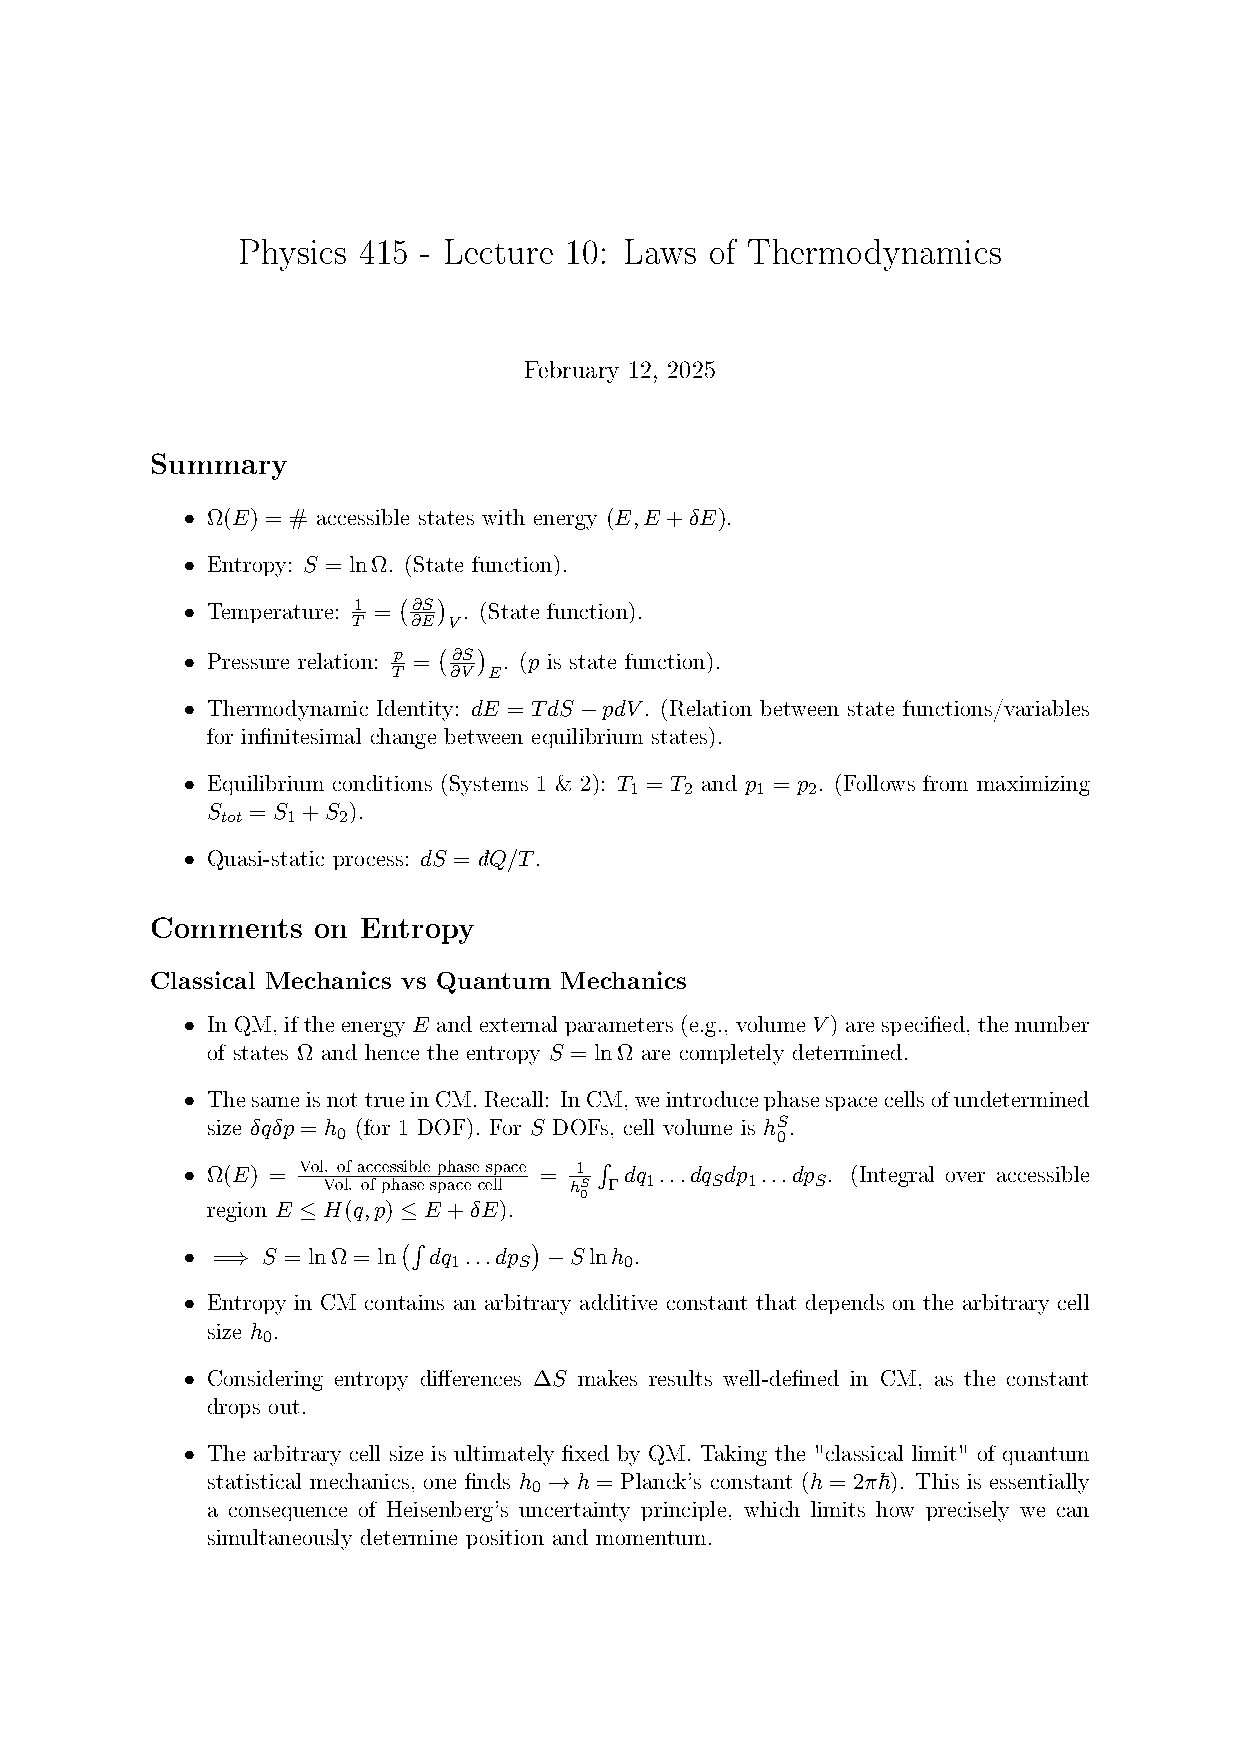
\includepdf[pages=-]{10.pdf}
\cleardoublepage
\phantomsection
\addcontentsline{toc}{chapter}{Lecture 11}
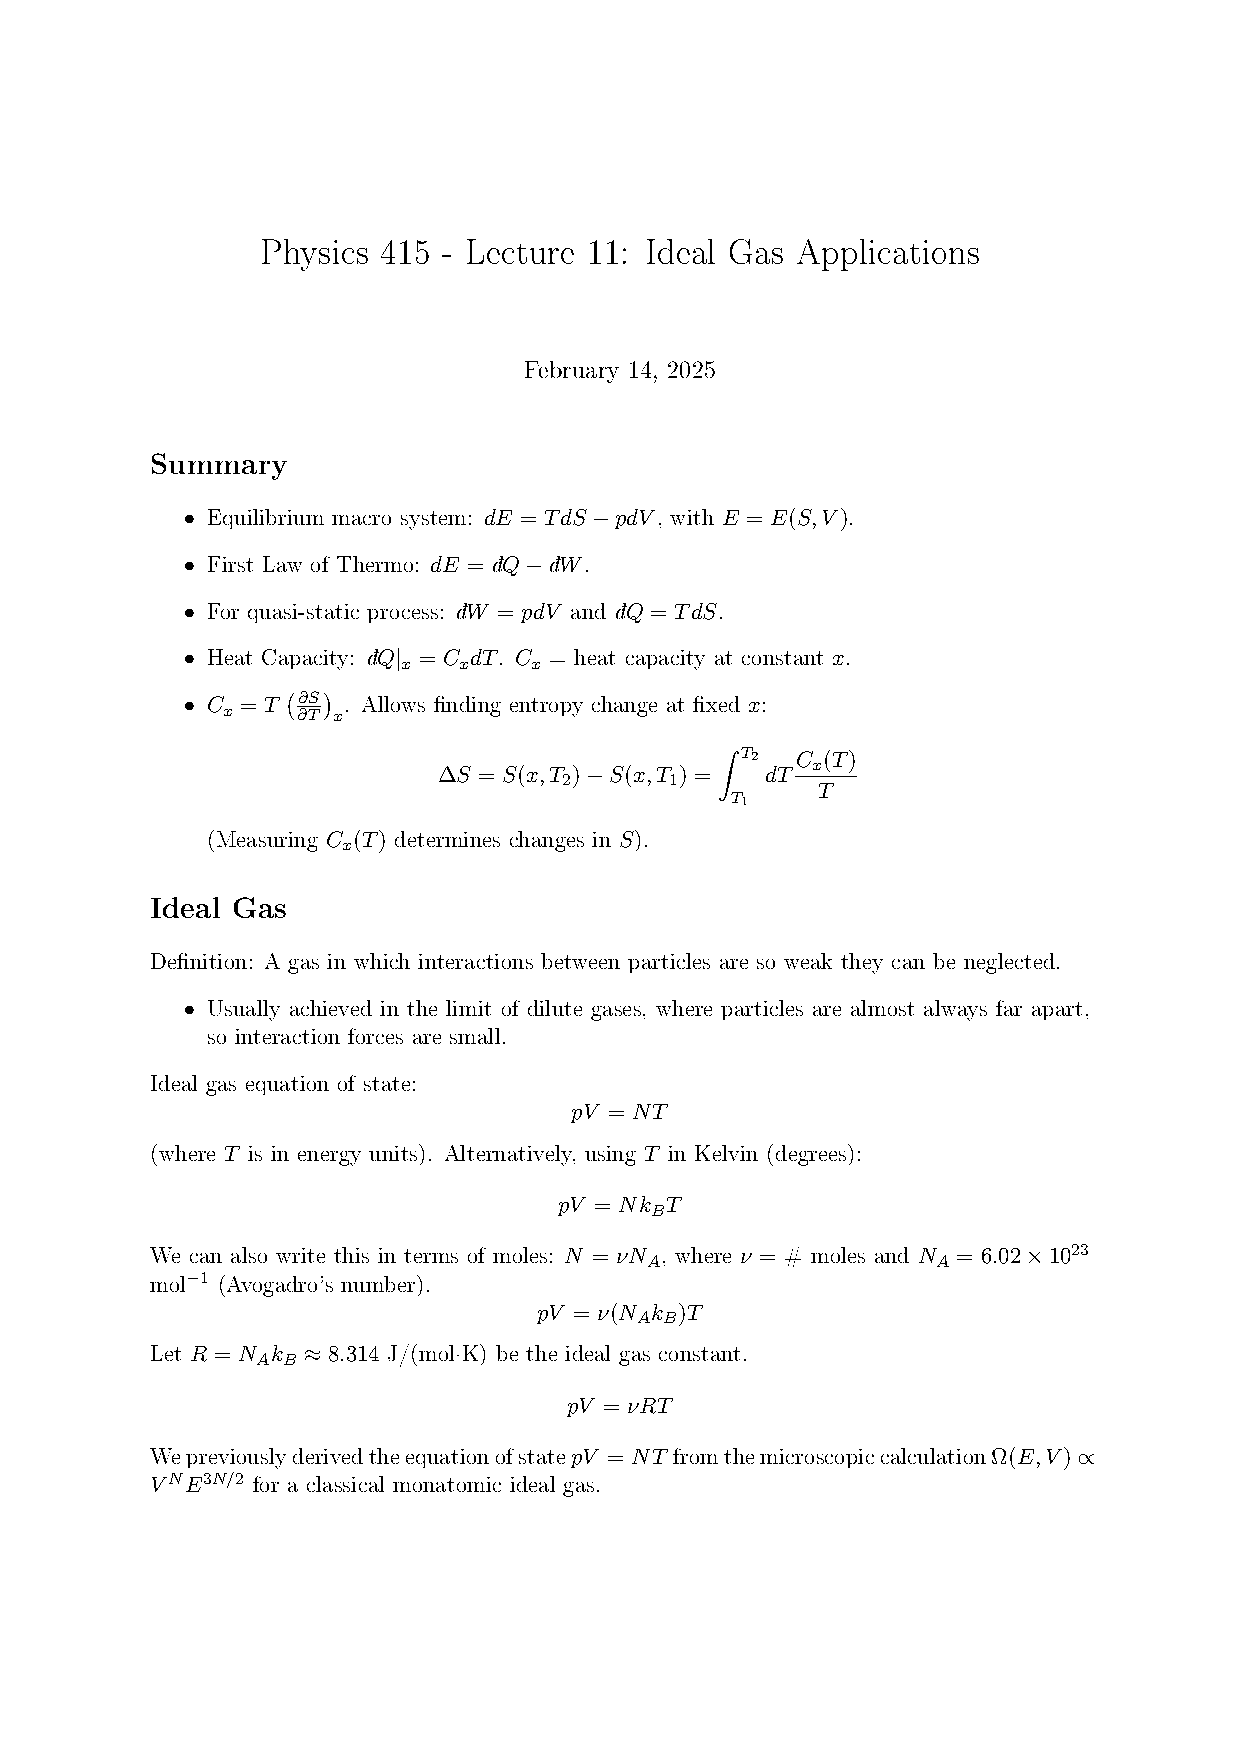
\includepdf[pages=-]{11.pdf}
\cleardoublepage
\phantomsection
\addcontentsline{toc}{chapter}{Lecture 12}
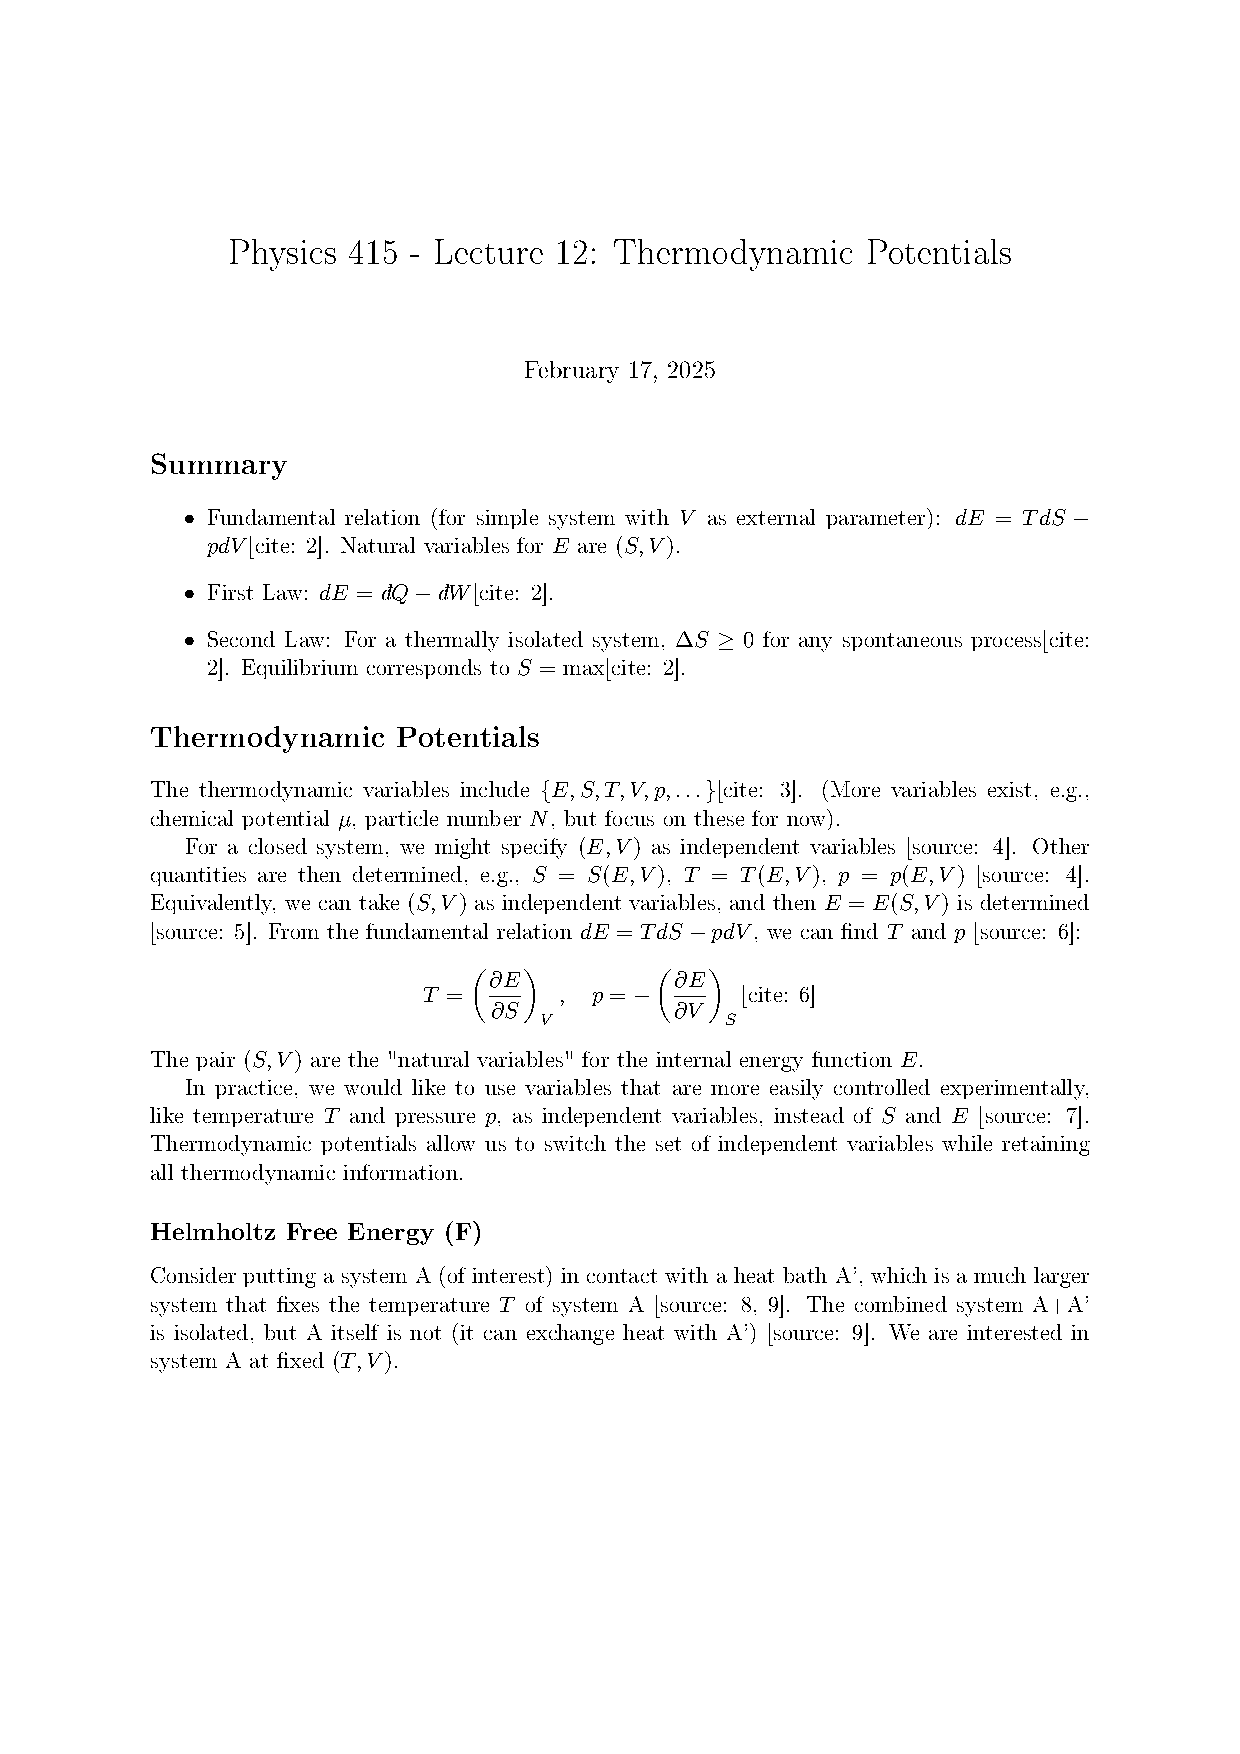
\includepdf[pages=-]{12.pdf}
\cleardoublepage
\phantomsection
\addcontentsline{toc}{chapter}{Lecture 13}
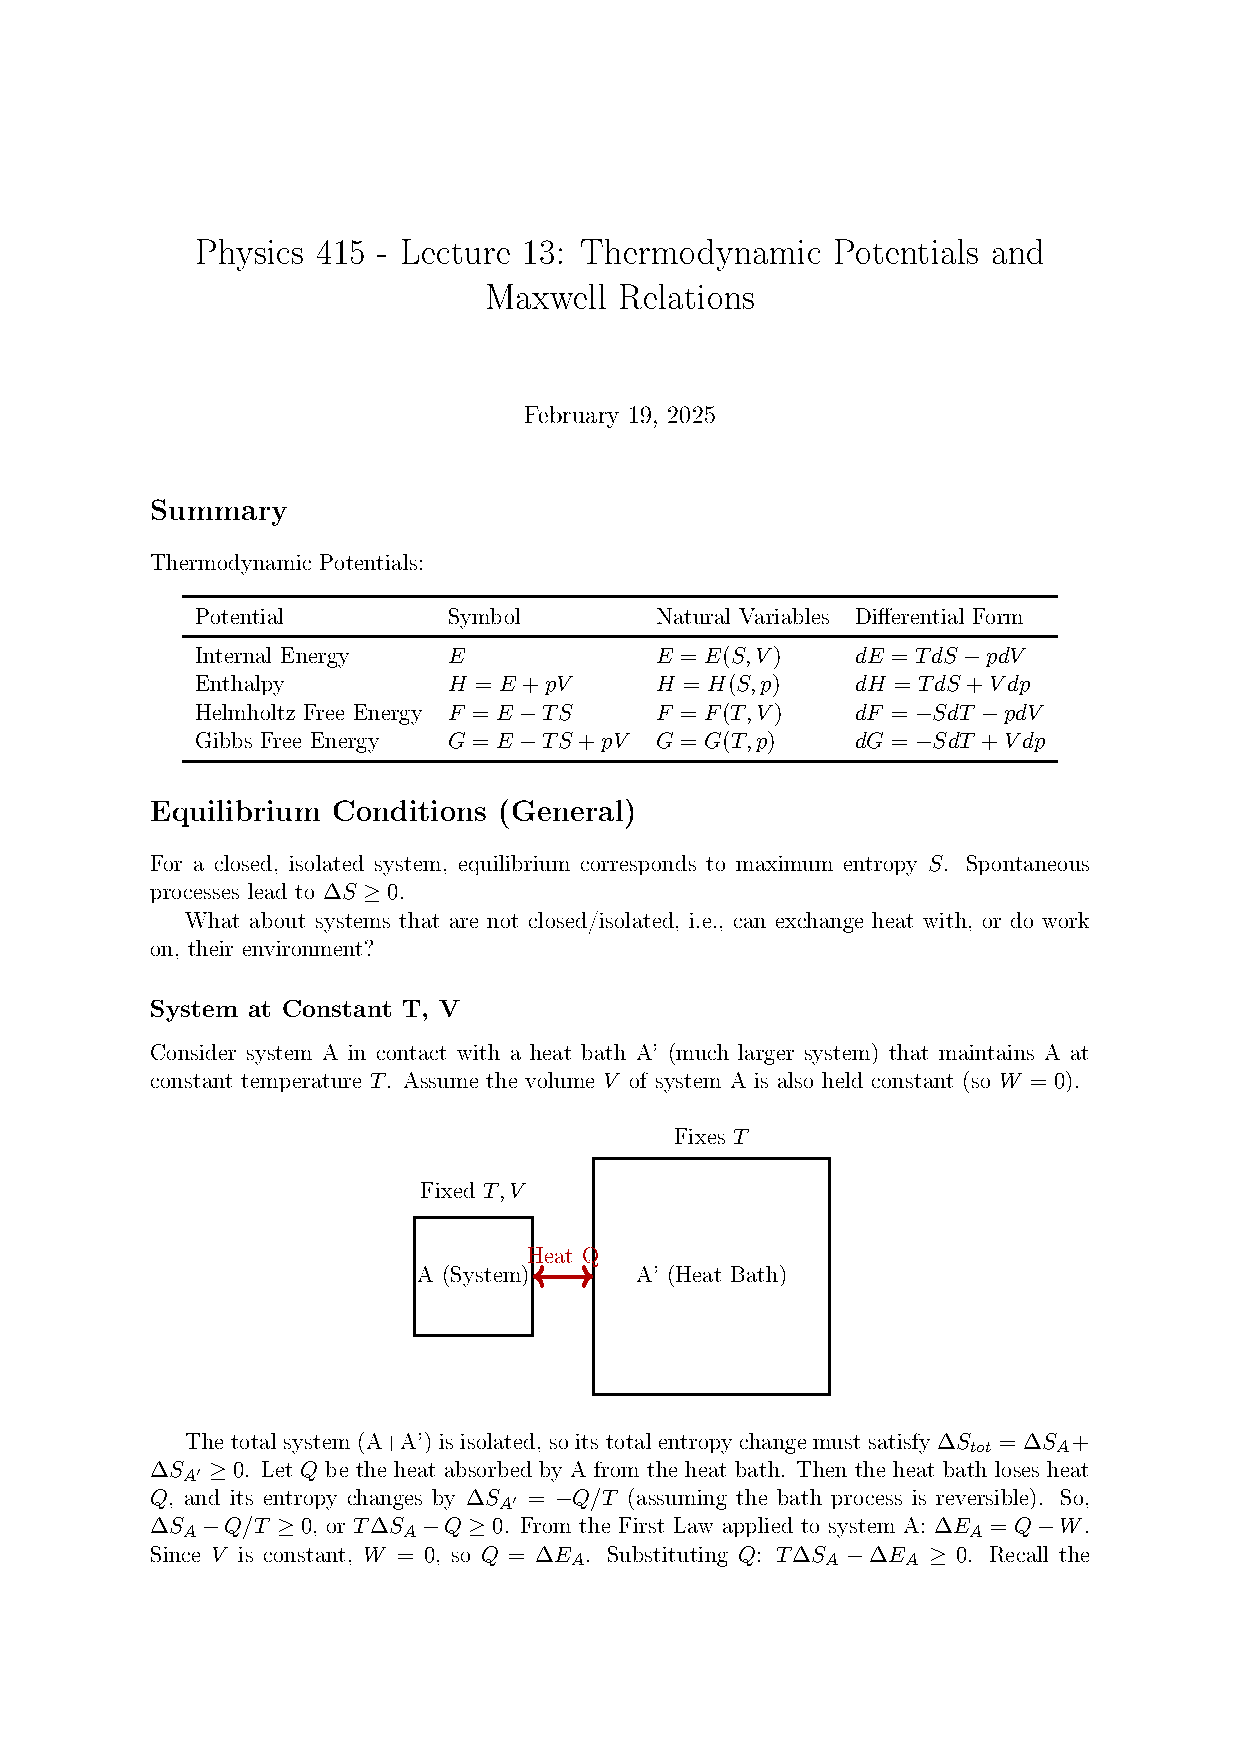
\includepdf[pages=-]{13.pdf}
\cleardoublepage
\phantomsection
\addcontentsline{toc}{chapter}{Lecture 14}
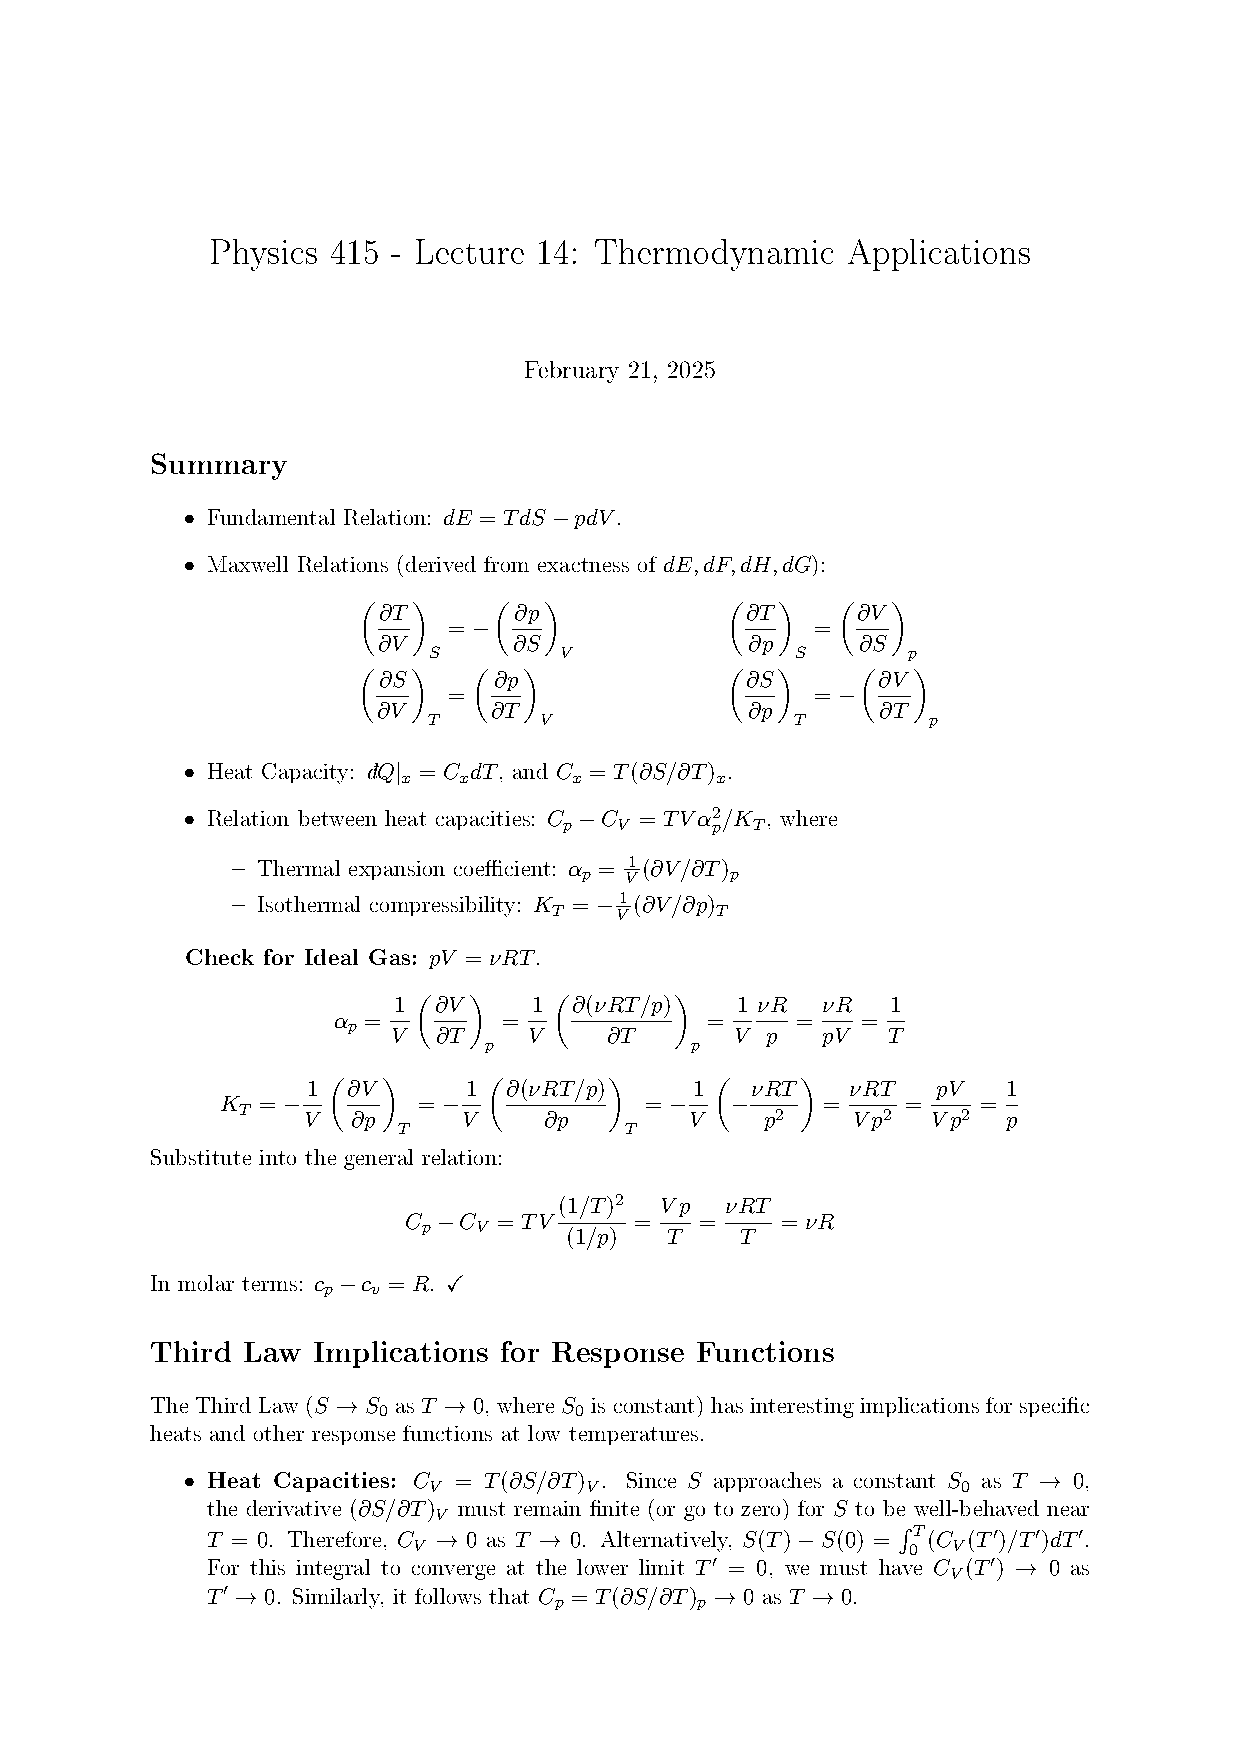
\includepdf[pages=-]{14.pdf}
\cleardoublepage
\phantomsection
\addcontentsline{toc}{chapter}{Lecture 15}
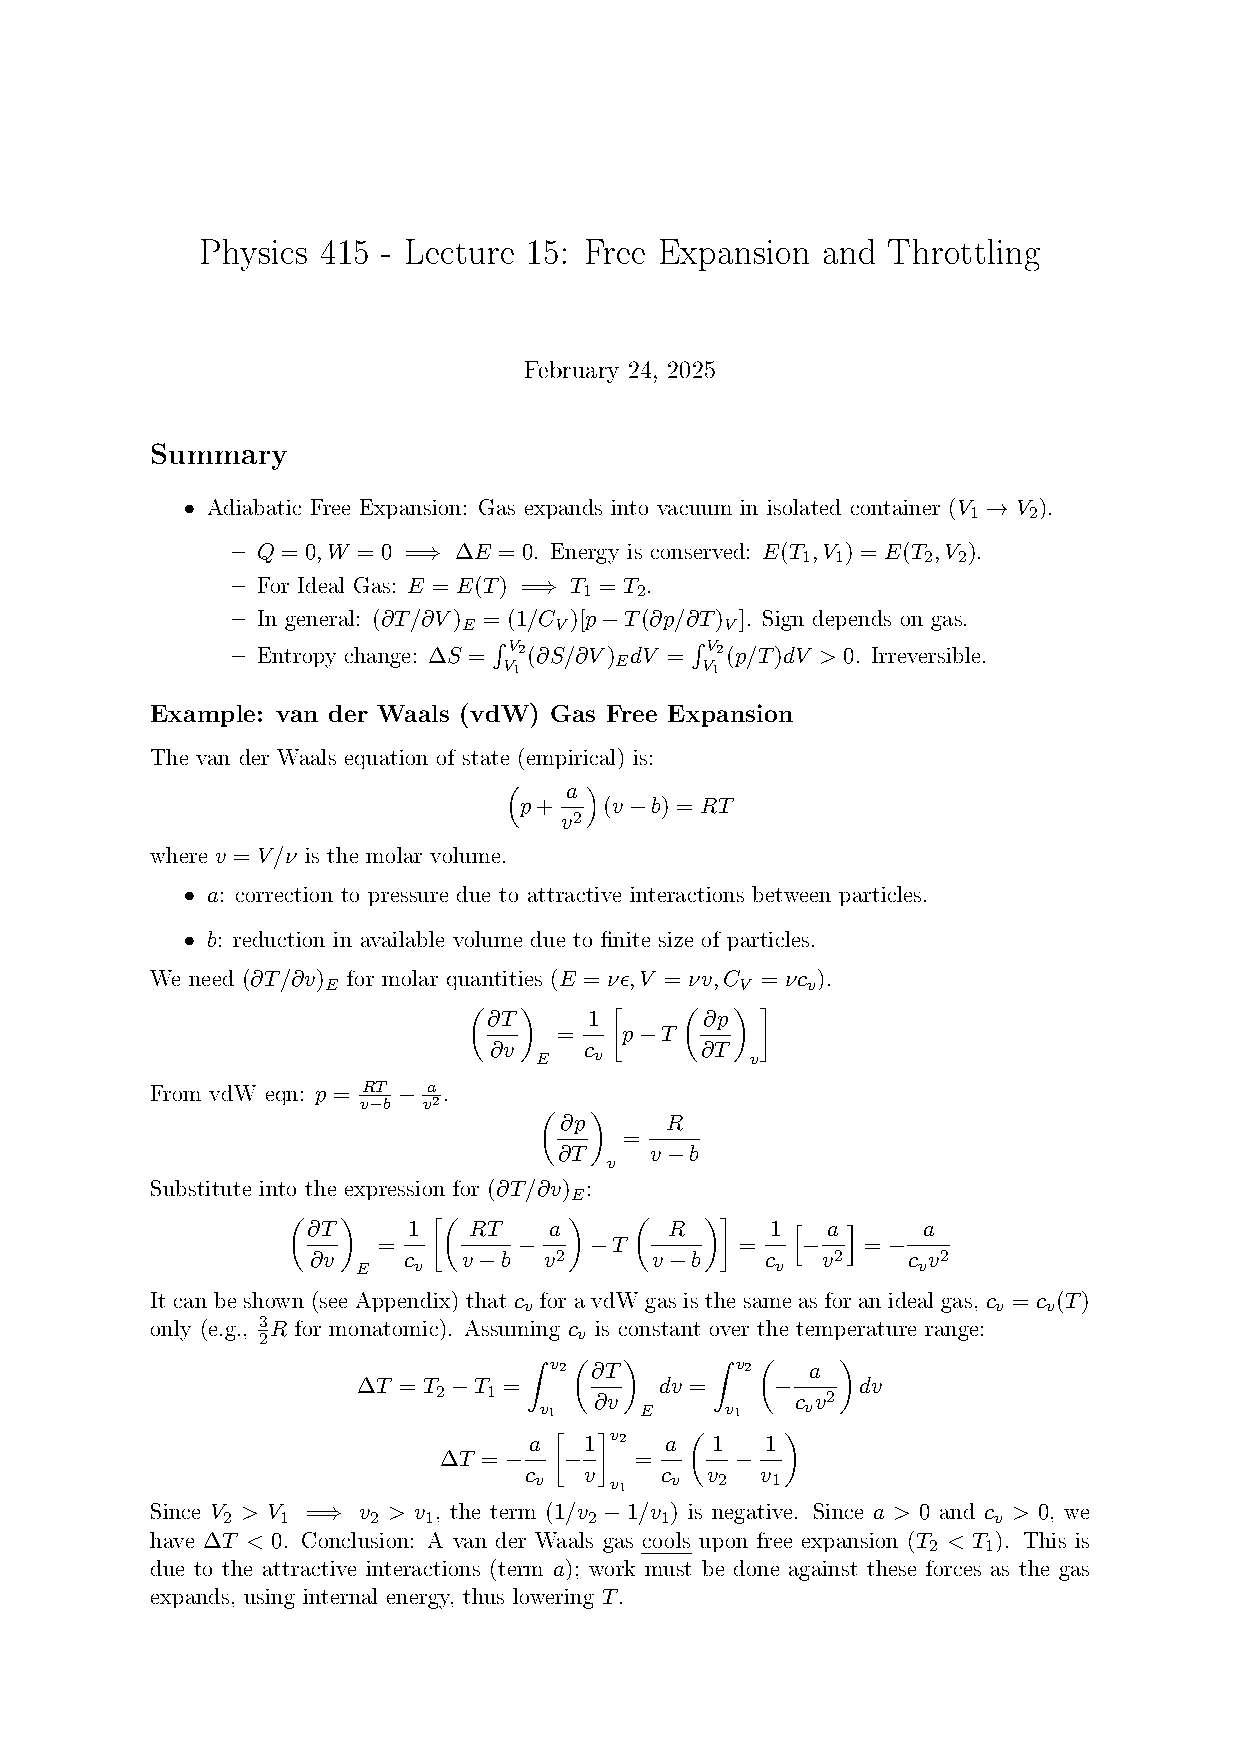
\includepdf[pages=-]{15.pdf}
\cleardoublepage
\phantomsection
\addcontentsline{toc}{chapter}{Lecture 16}
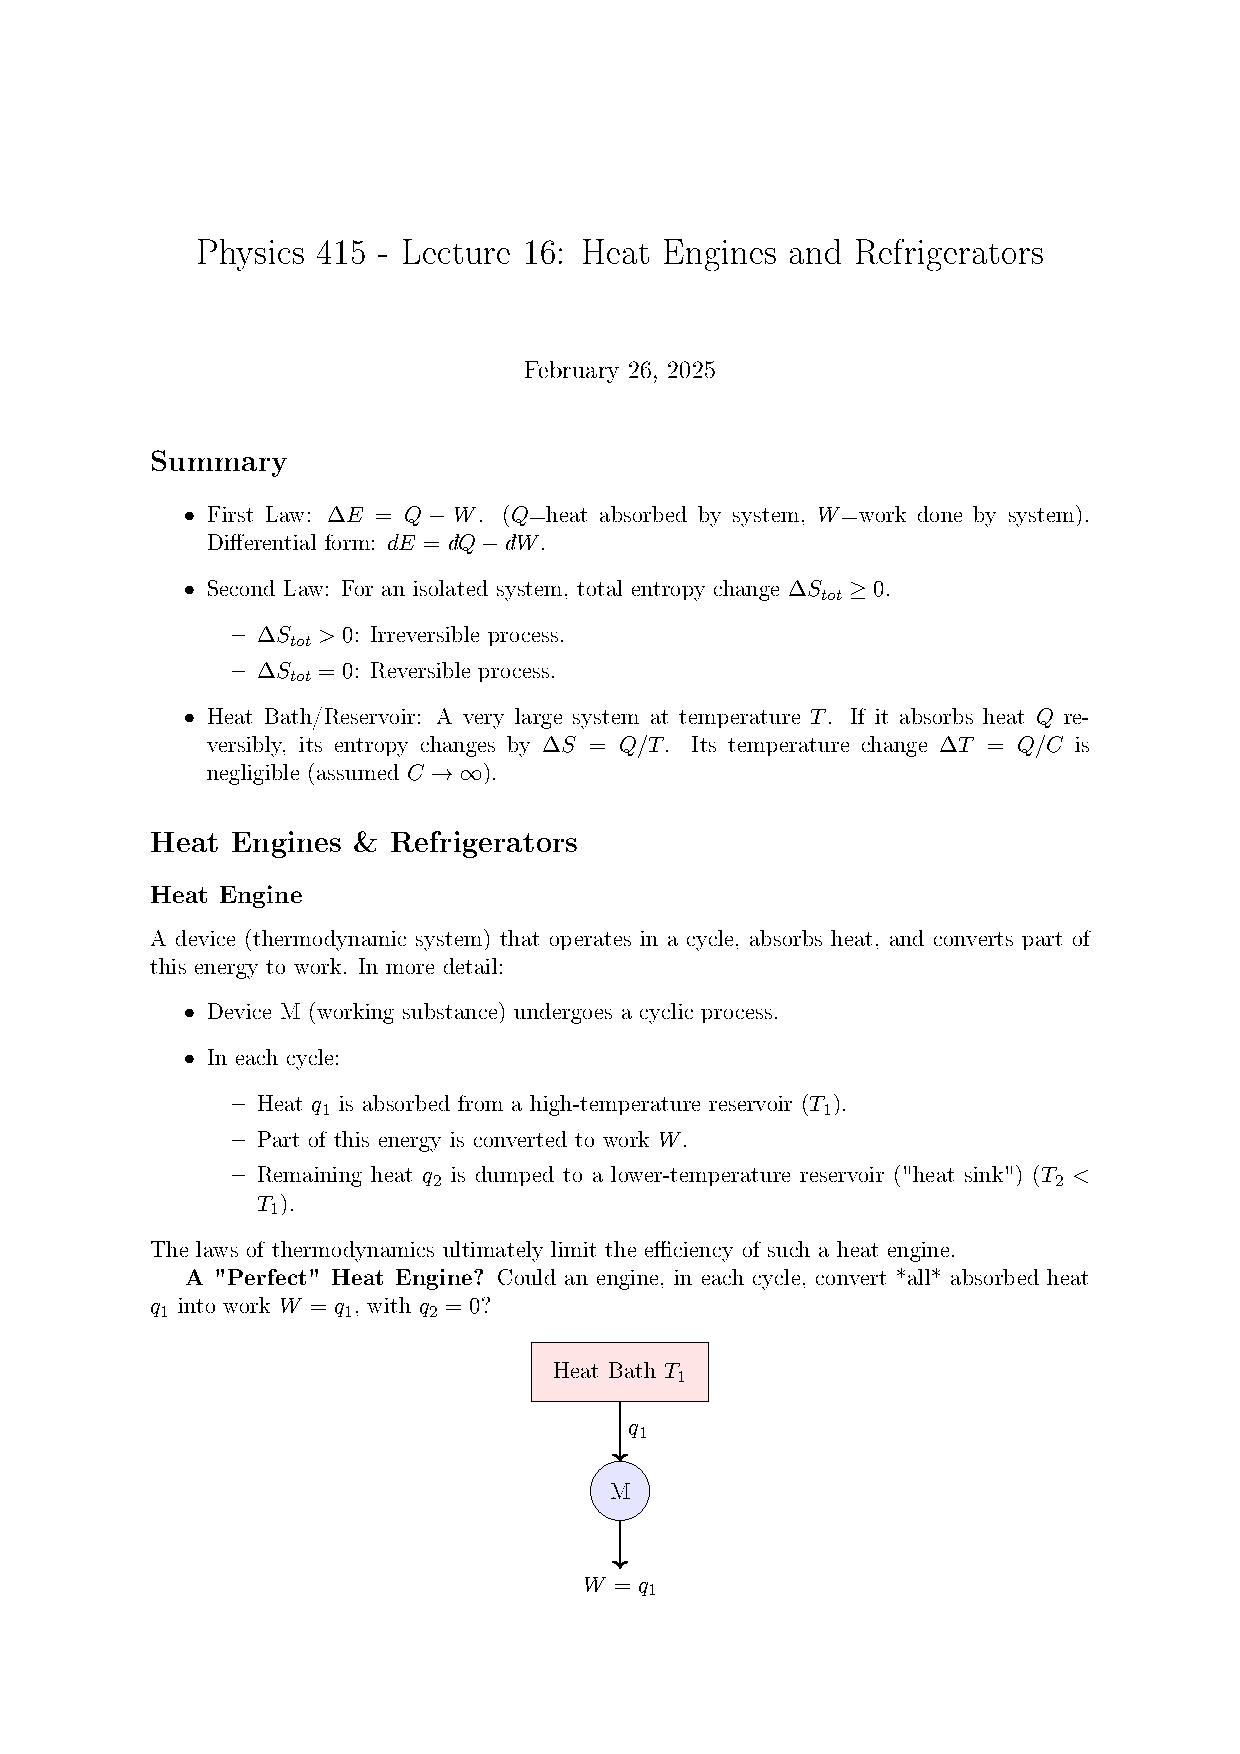
\includepdf[pages=-]{16.pdf}

% Skip 17.pdf
\cleardoublepage

% Include files 18 through 25
\phantomsection
\addcontentsline{toc}{chapter}{Lecture 18}
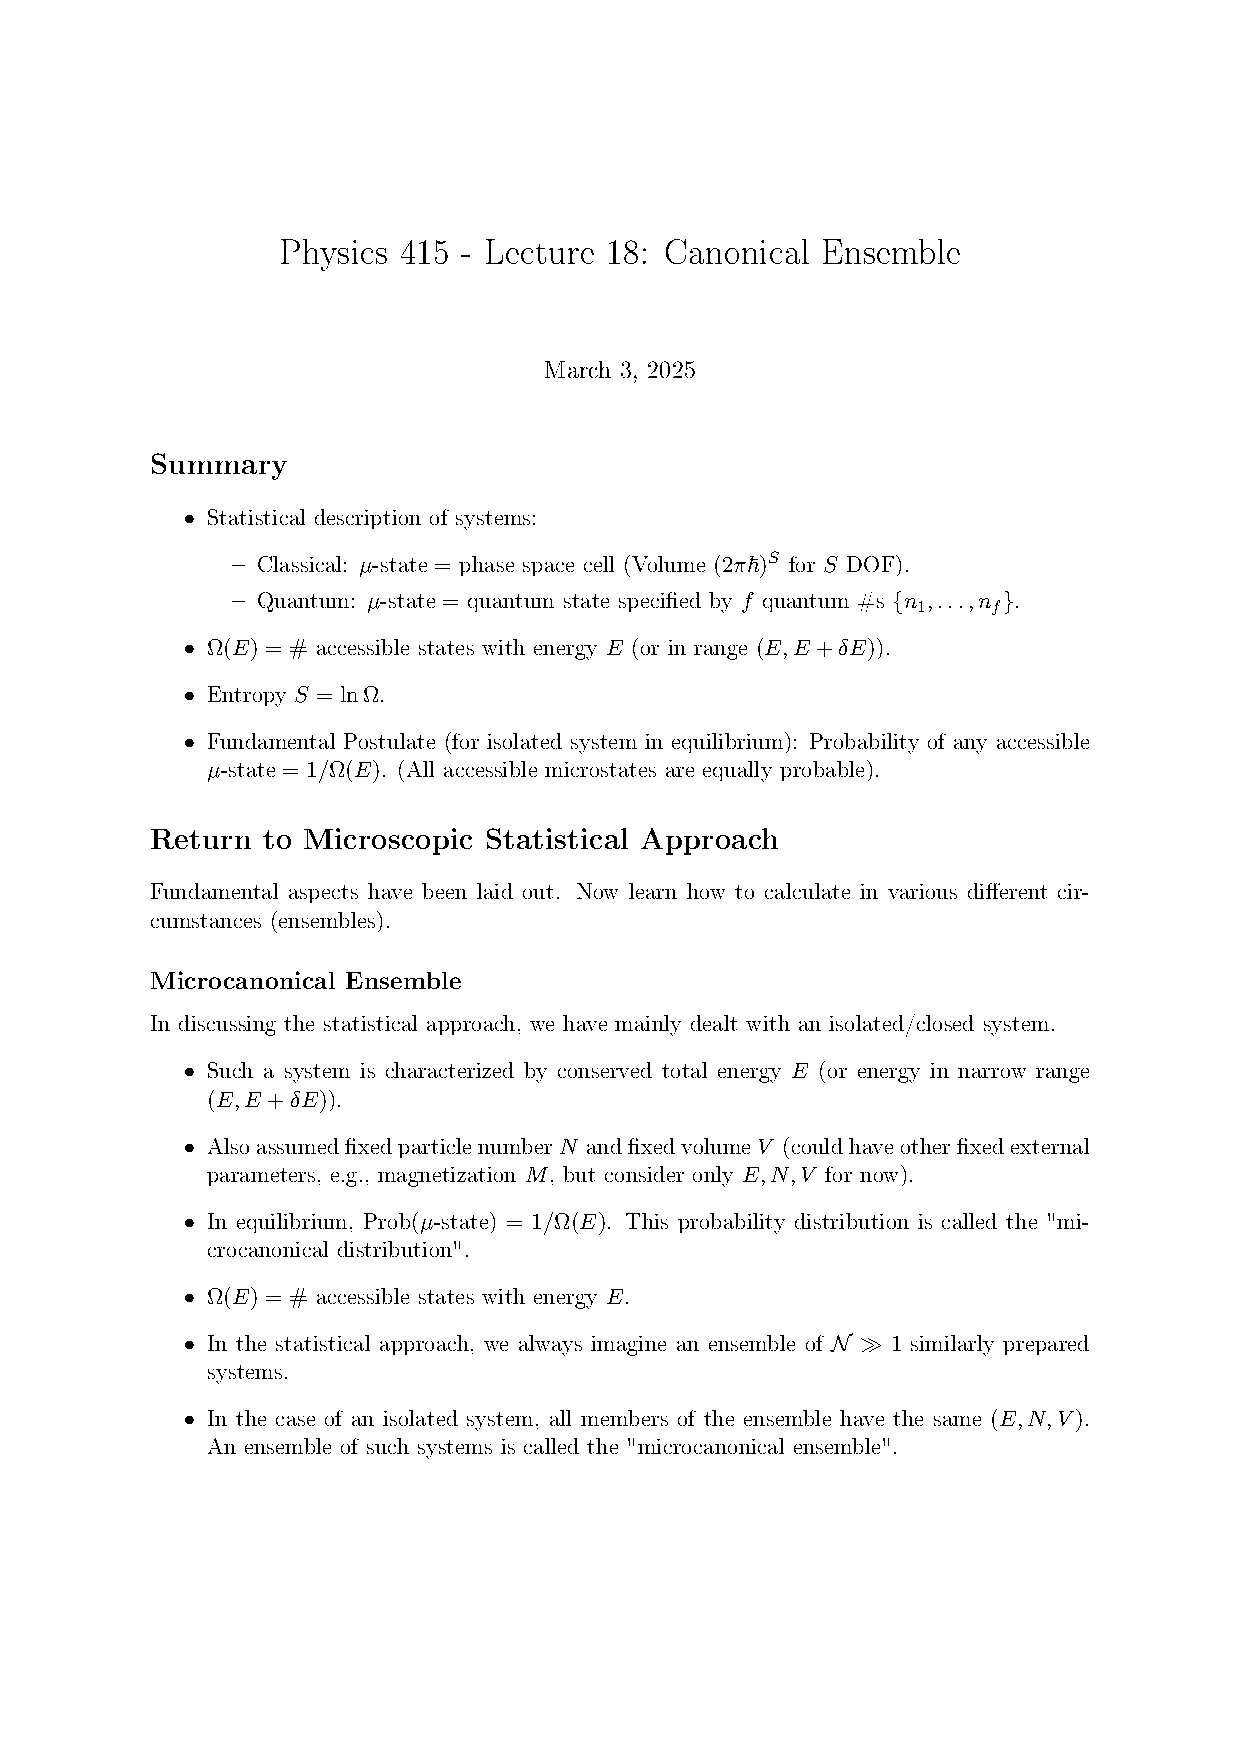
\includepdf[pages=-]{18.pdf}
\cleardoublepage
\phantomsection
\addcontentsline{toc}{chapter}{Lecture 19}
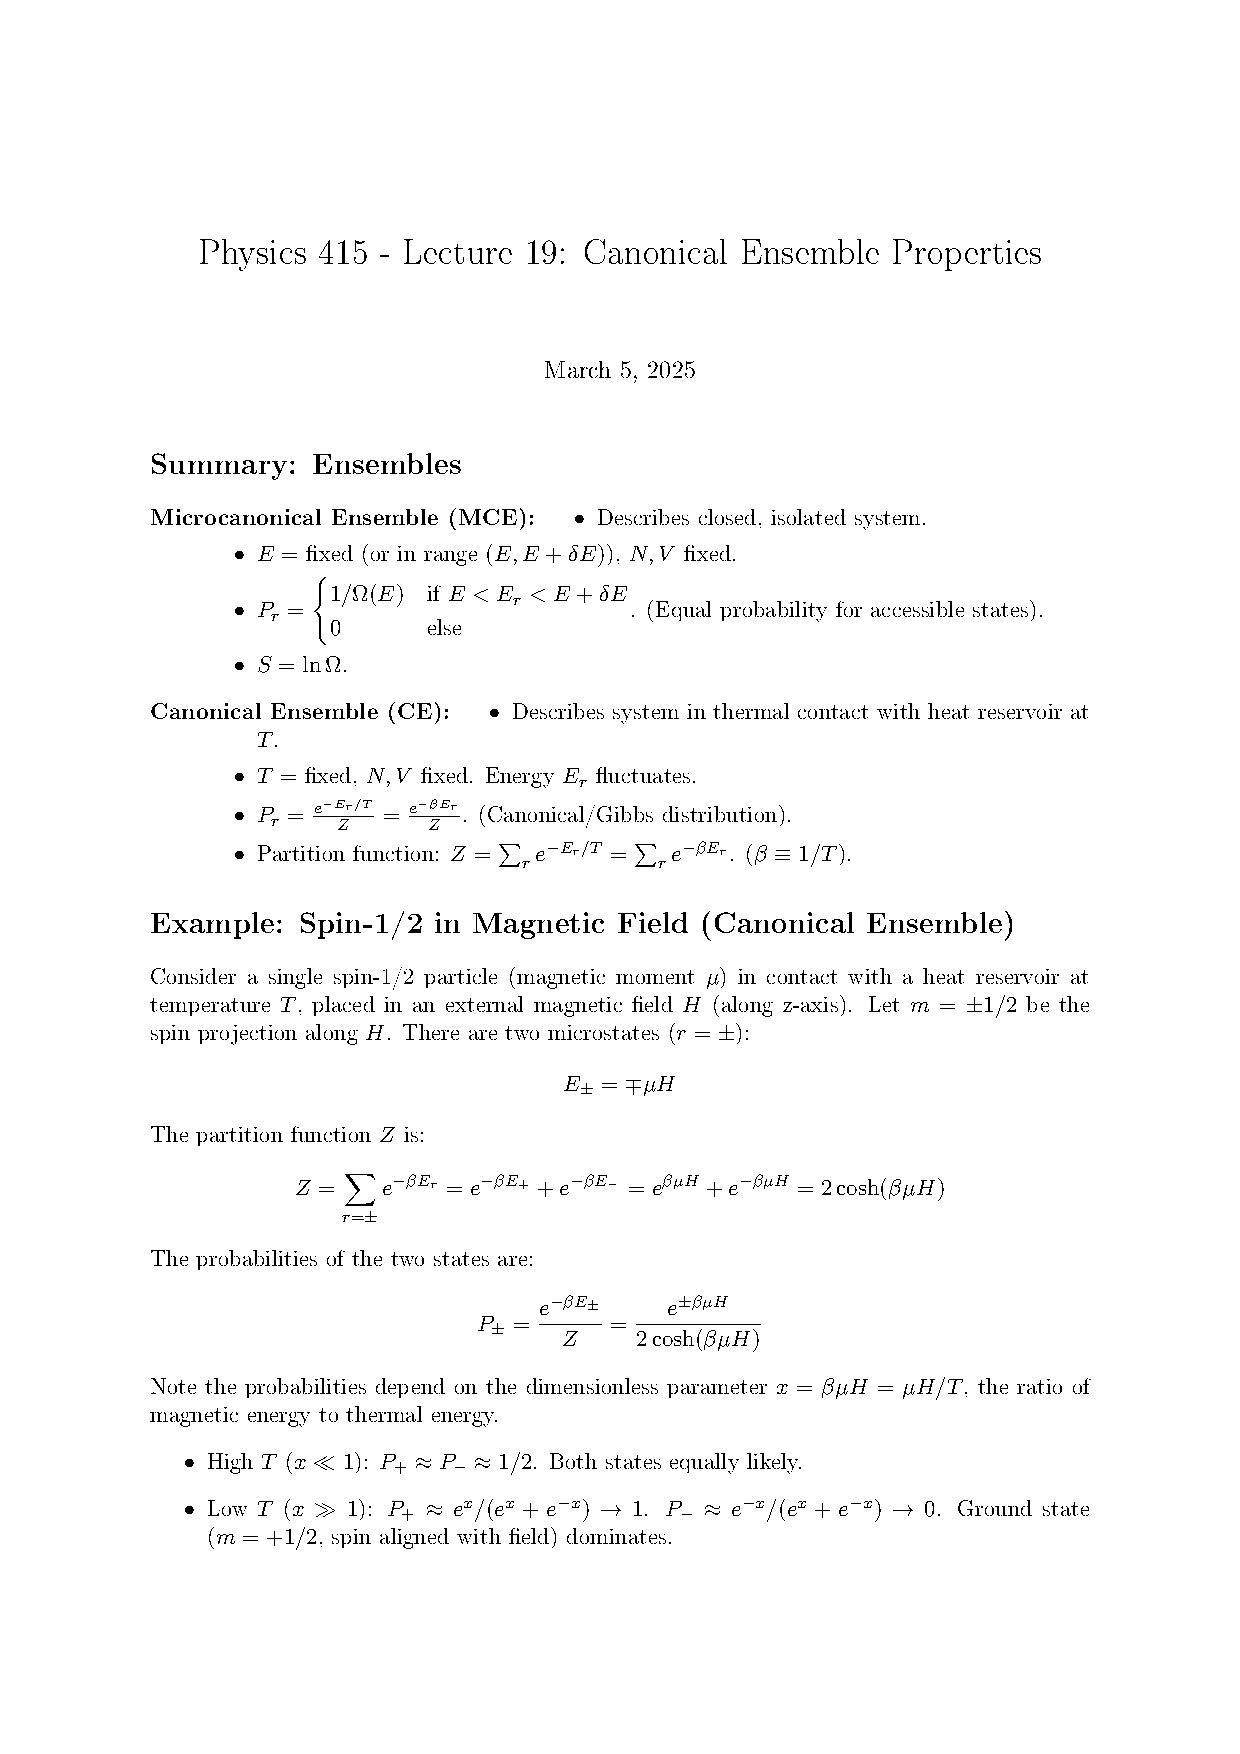
\includepdf[pages=-]{19.pdf}
\cleardoublepage
\phantomsection
\addcontentsline{toc}{chapter}{Lecture 20}
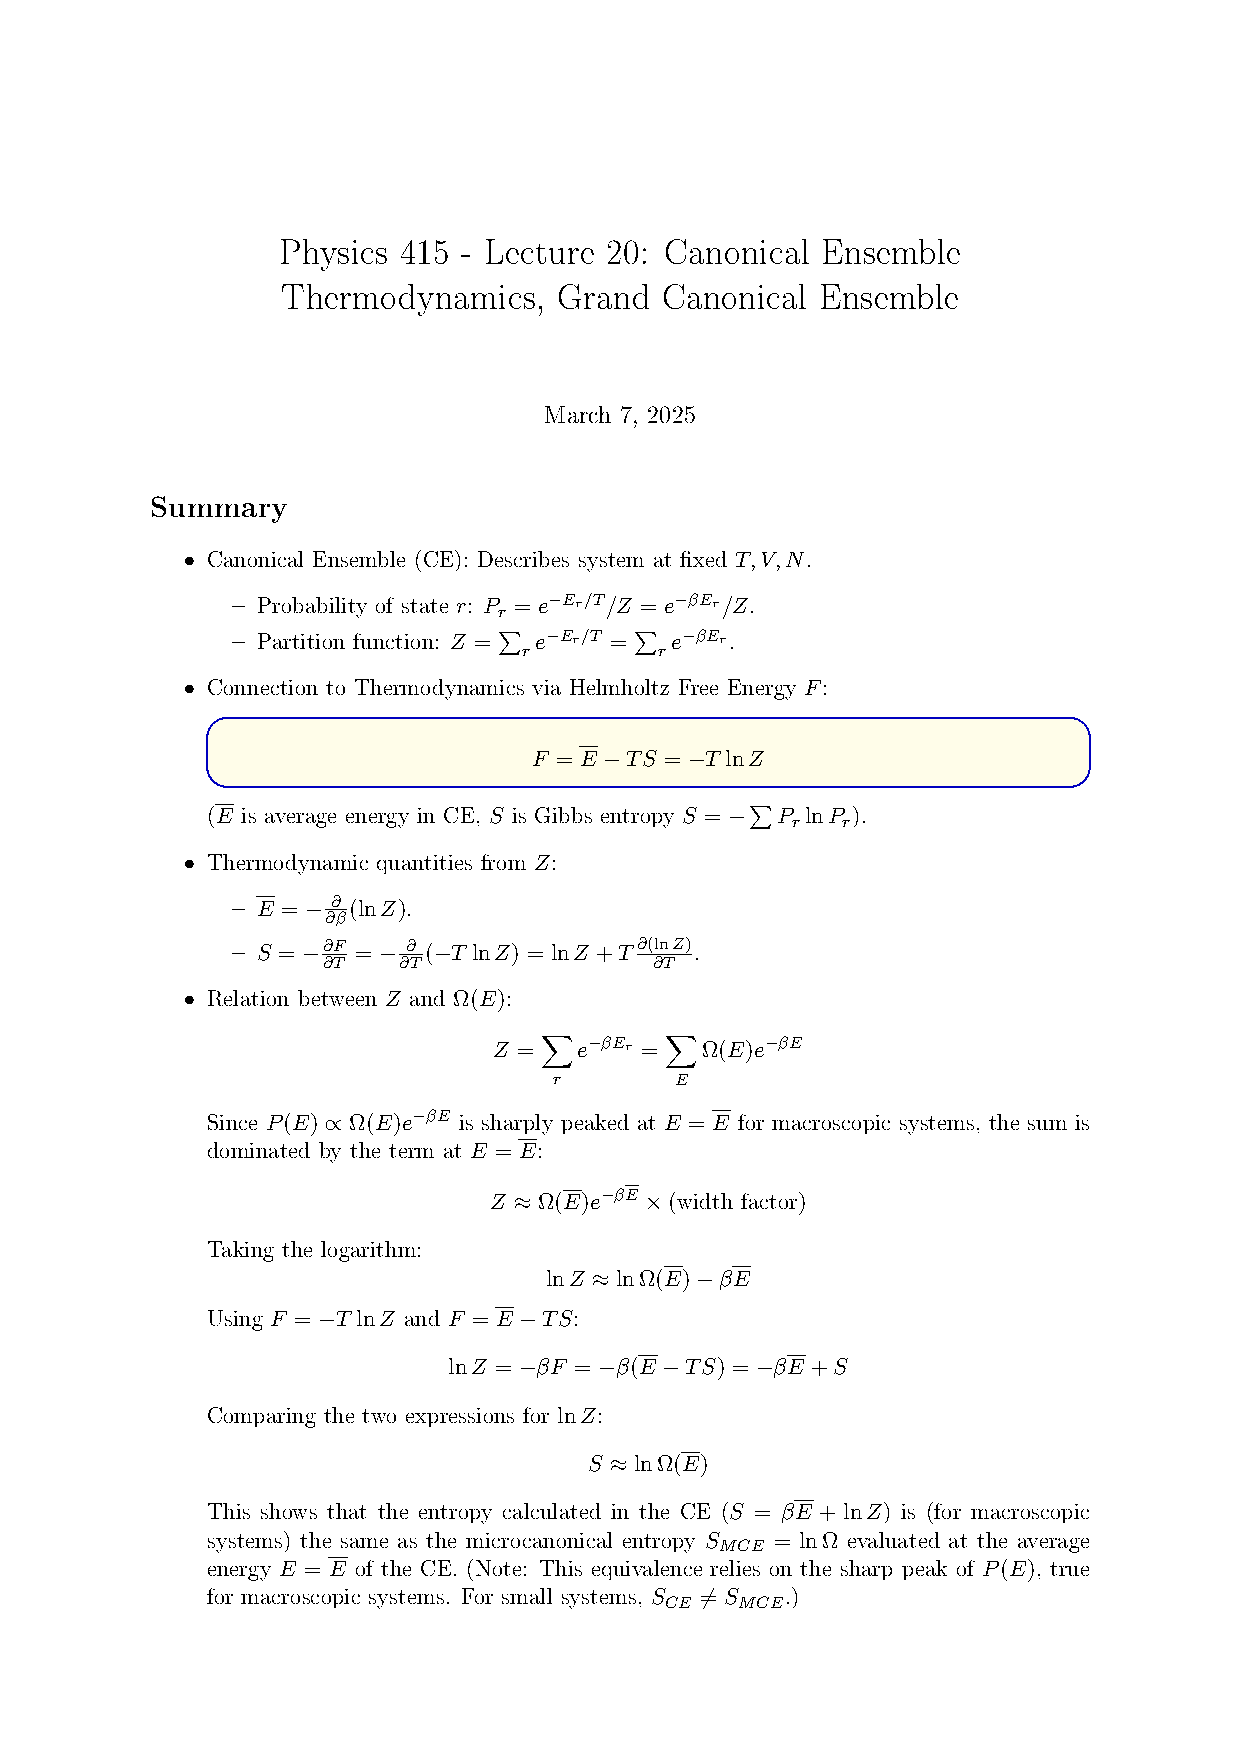
\includepdf[pages=-]{20.pdf}
\cleardoublepage
\phantomsection
\addcontentsline{toc}{chapter}{Lecture 21}
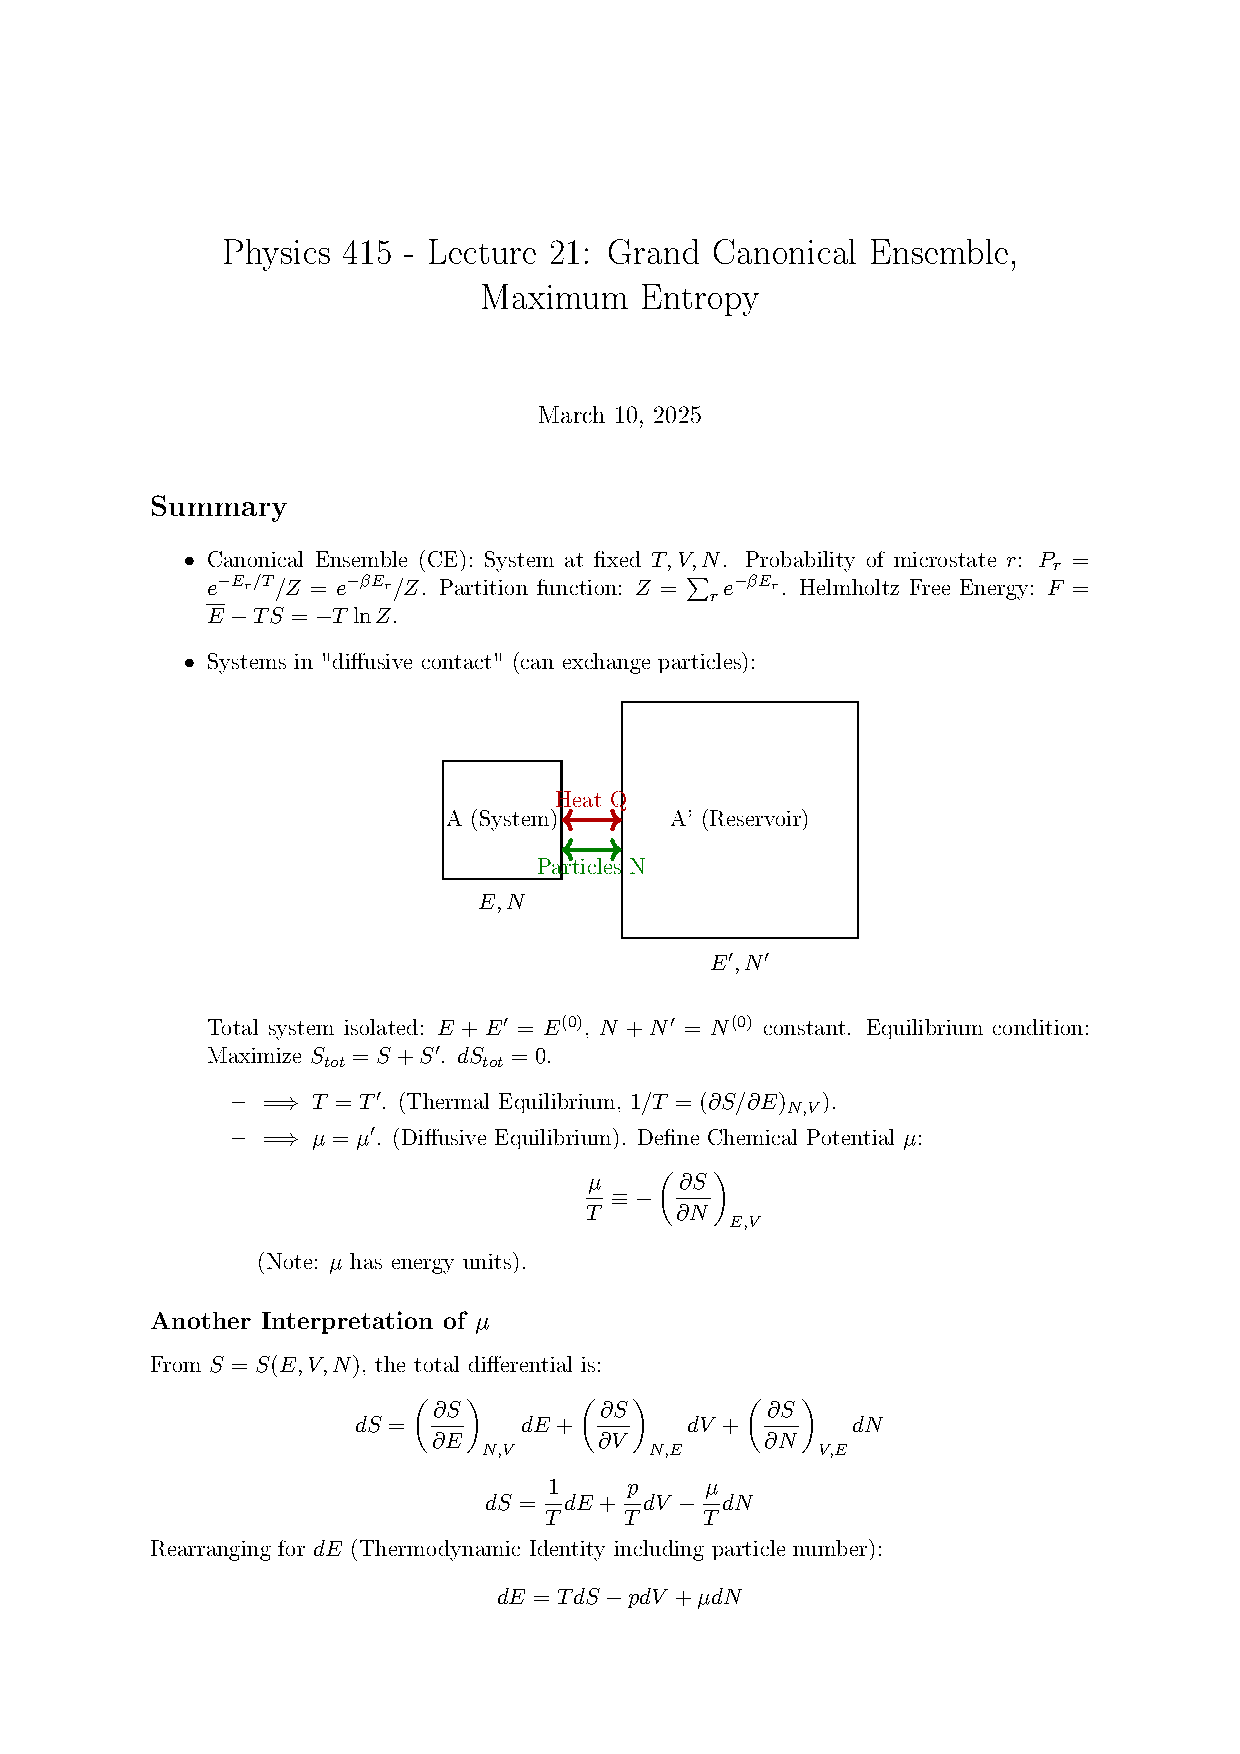
\includepdf[pages=-]{21.pdf}
\cleardoublepage
\phantomsection
\addcontentsline{toc}{chapter}{Lecture 22}
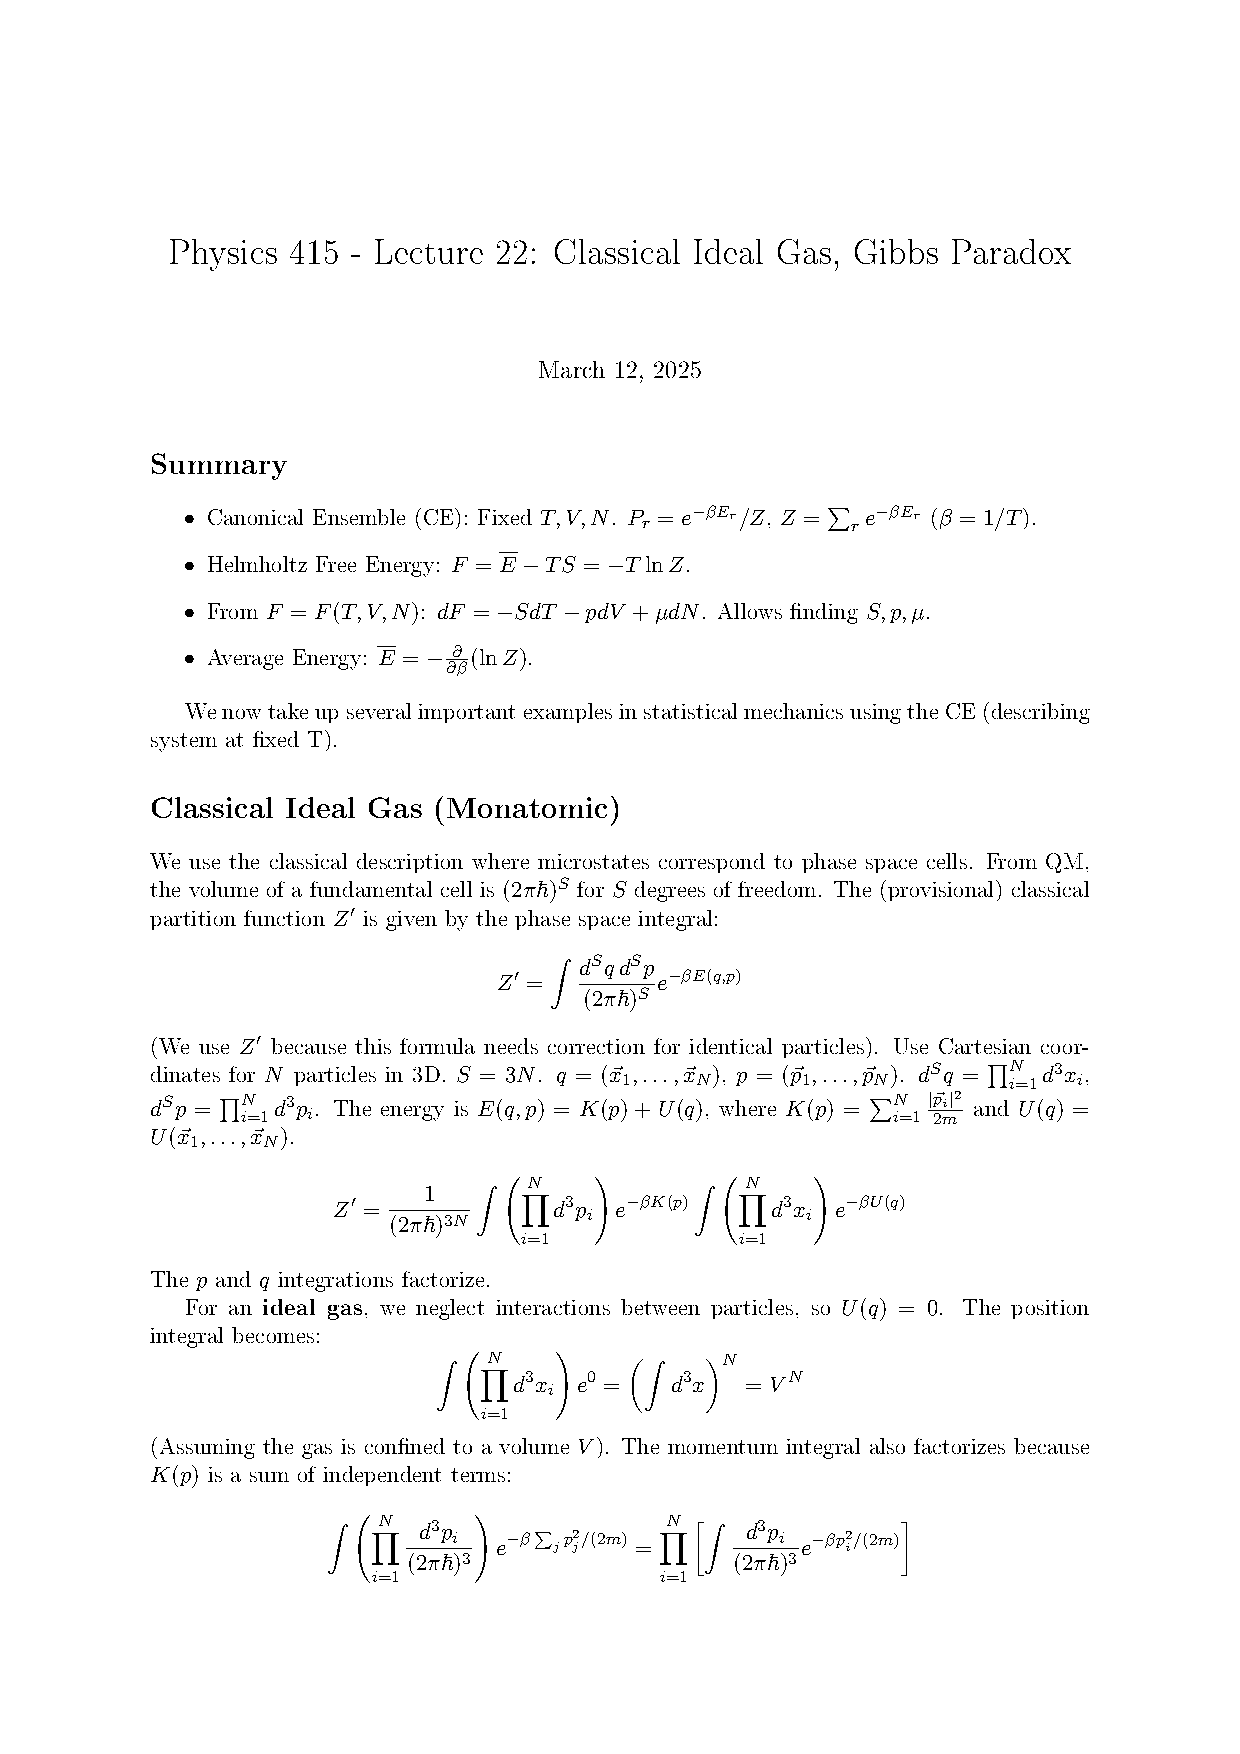
\includepdf[pages=-]{22.pdf}
\cleardoublepage
\phantomsection
\addcontentsline{toc}{chapter}{Lecture 23}
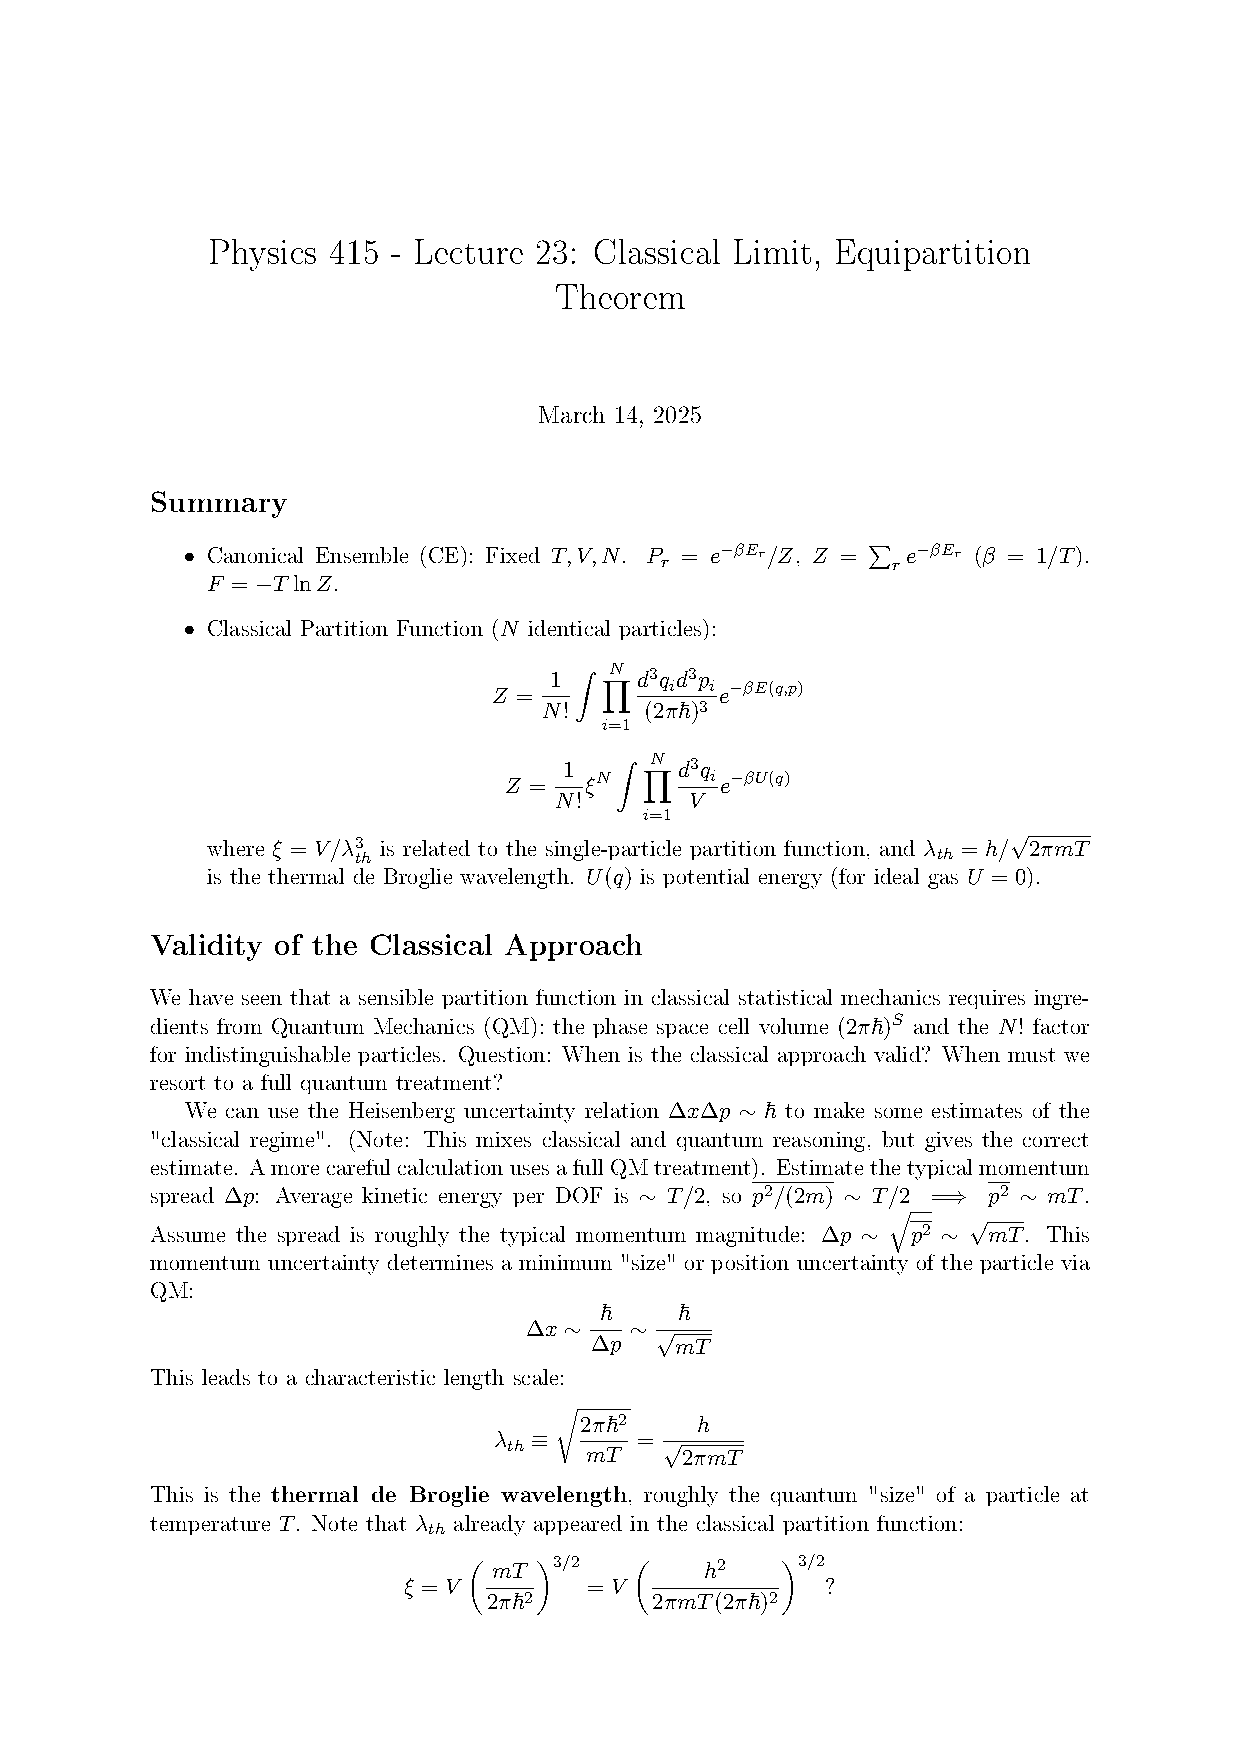
\includepdf[pages=-]{23.pdf}
\cleardoublepage
\phantomsection
\addcontentsline{toc}{chapter}{Lecture 24}
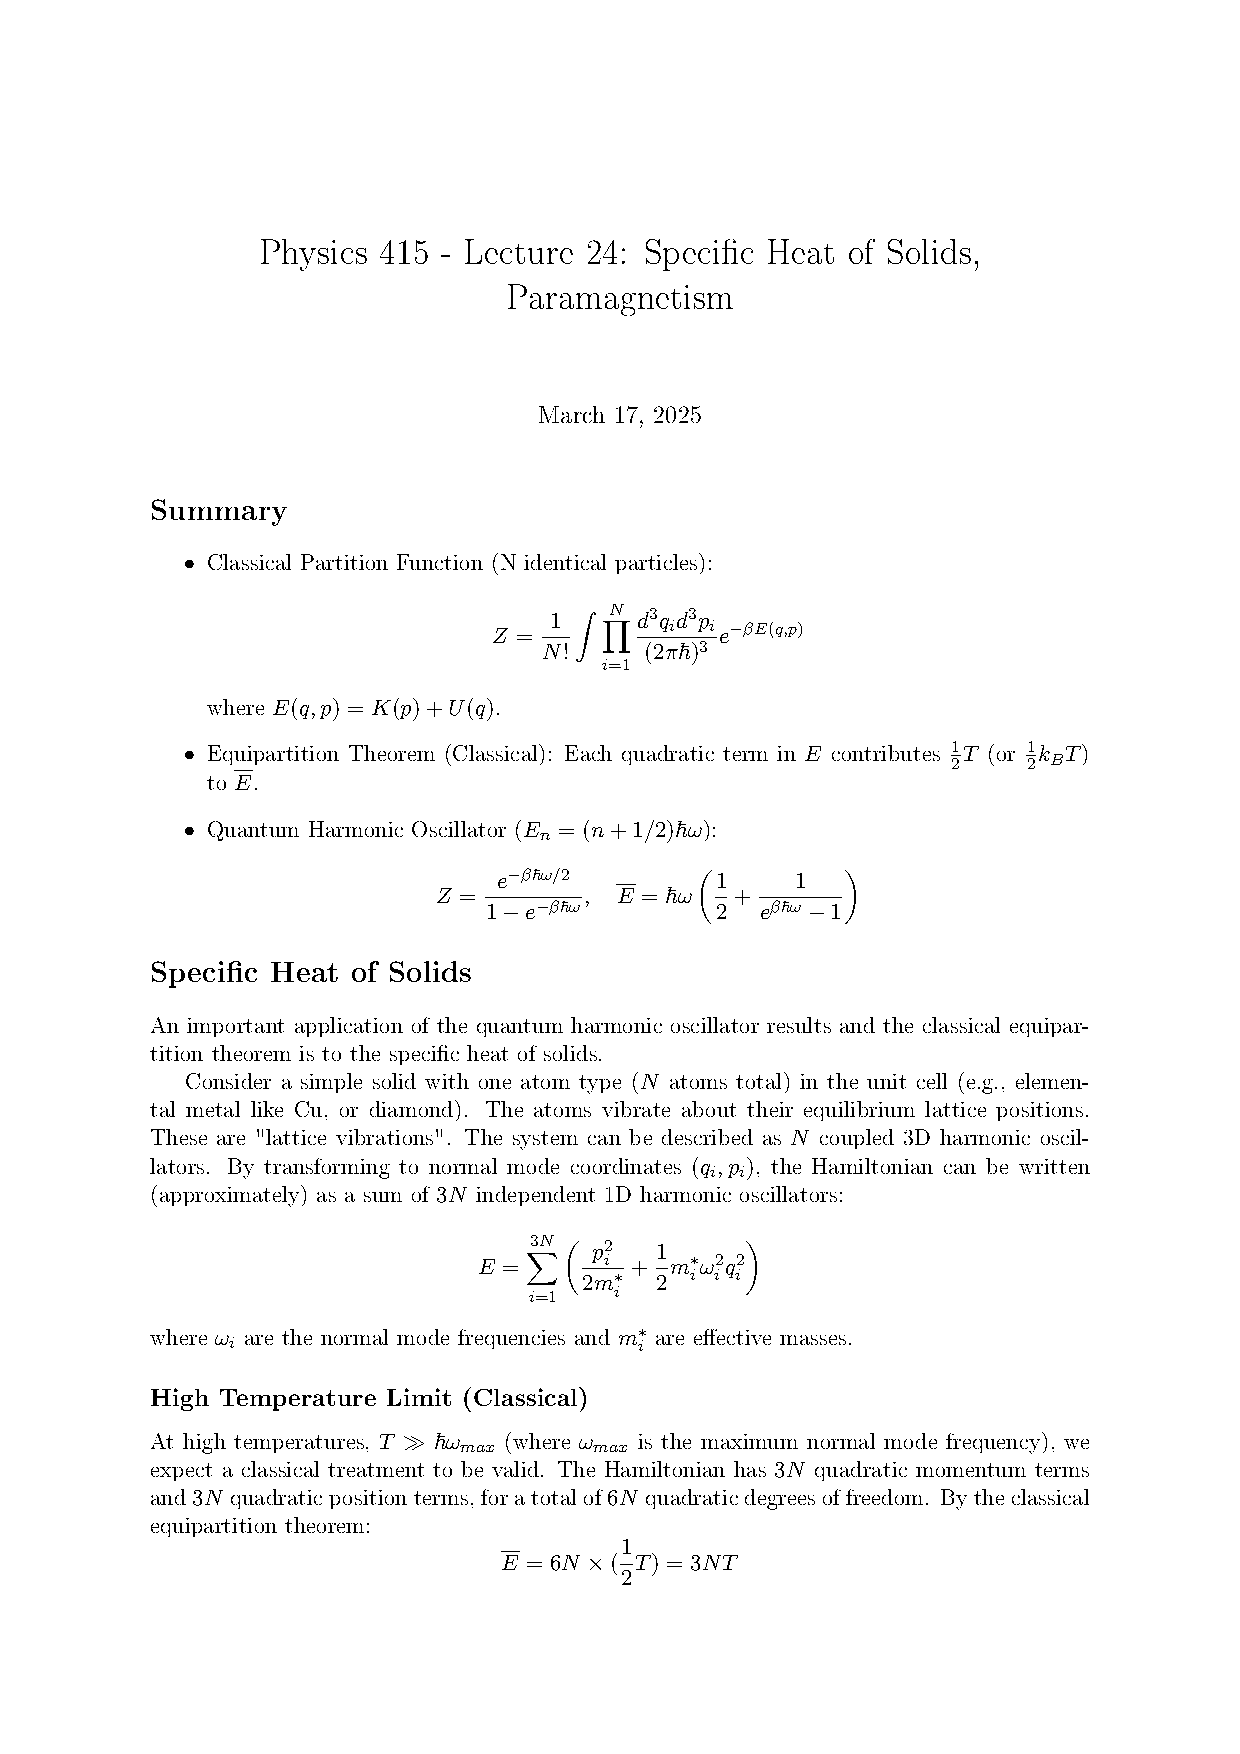
\includepdf[pages=-]{24.pdf}
\cleardoublepage
\phantomsection
\addcontentsline{toc}{chapter}{Lecture 25}
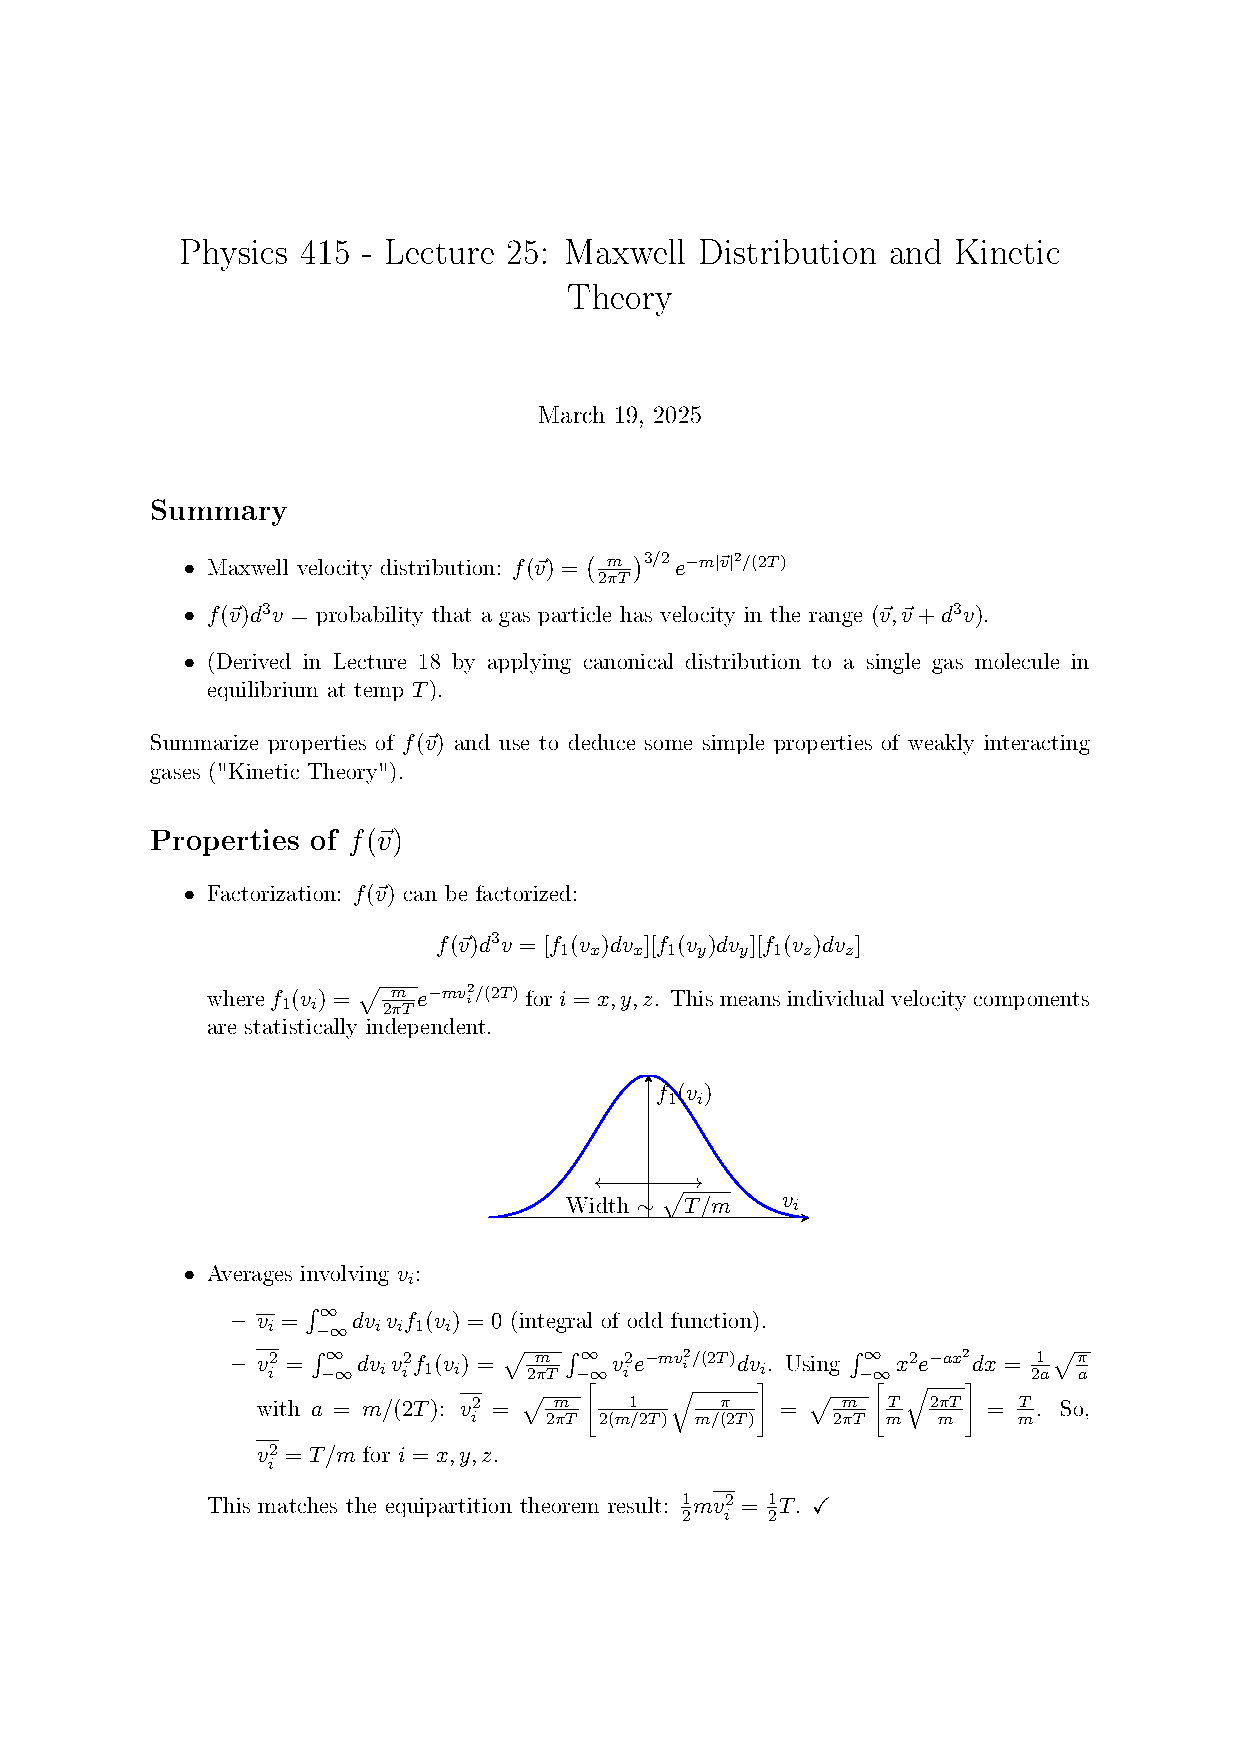
\includepdf[pages=-]{25.pdf}

% Skip 26.pdf
\cleardoublepage

% Include files 27 through 28
\phantomsection
\addcontentsline{toc}{chapter}{Lecture 27}
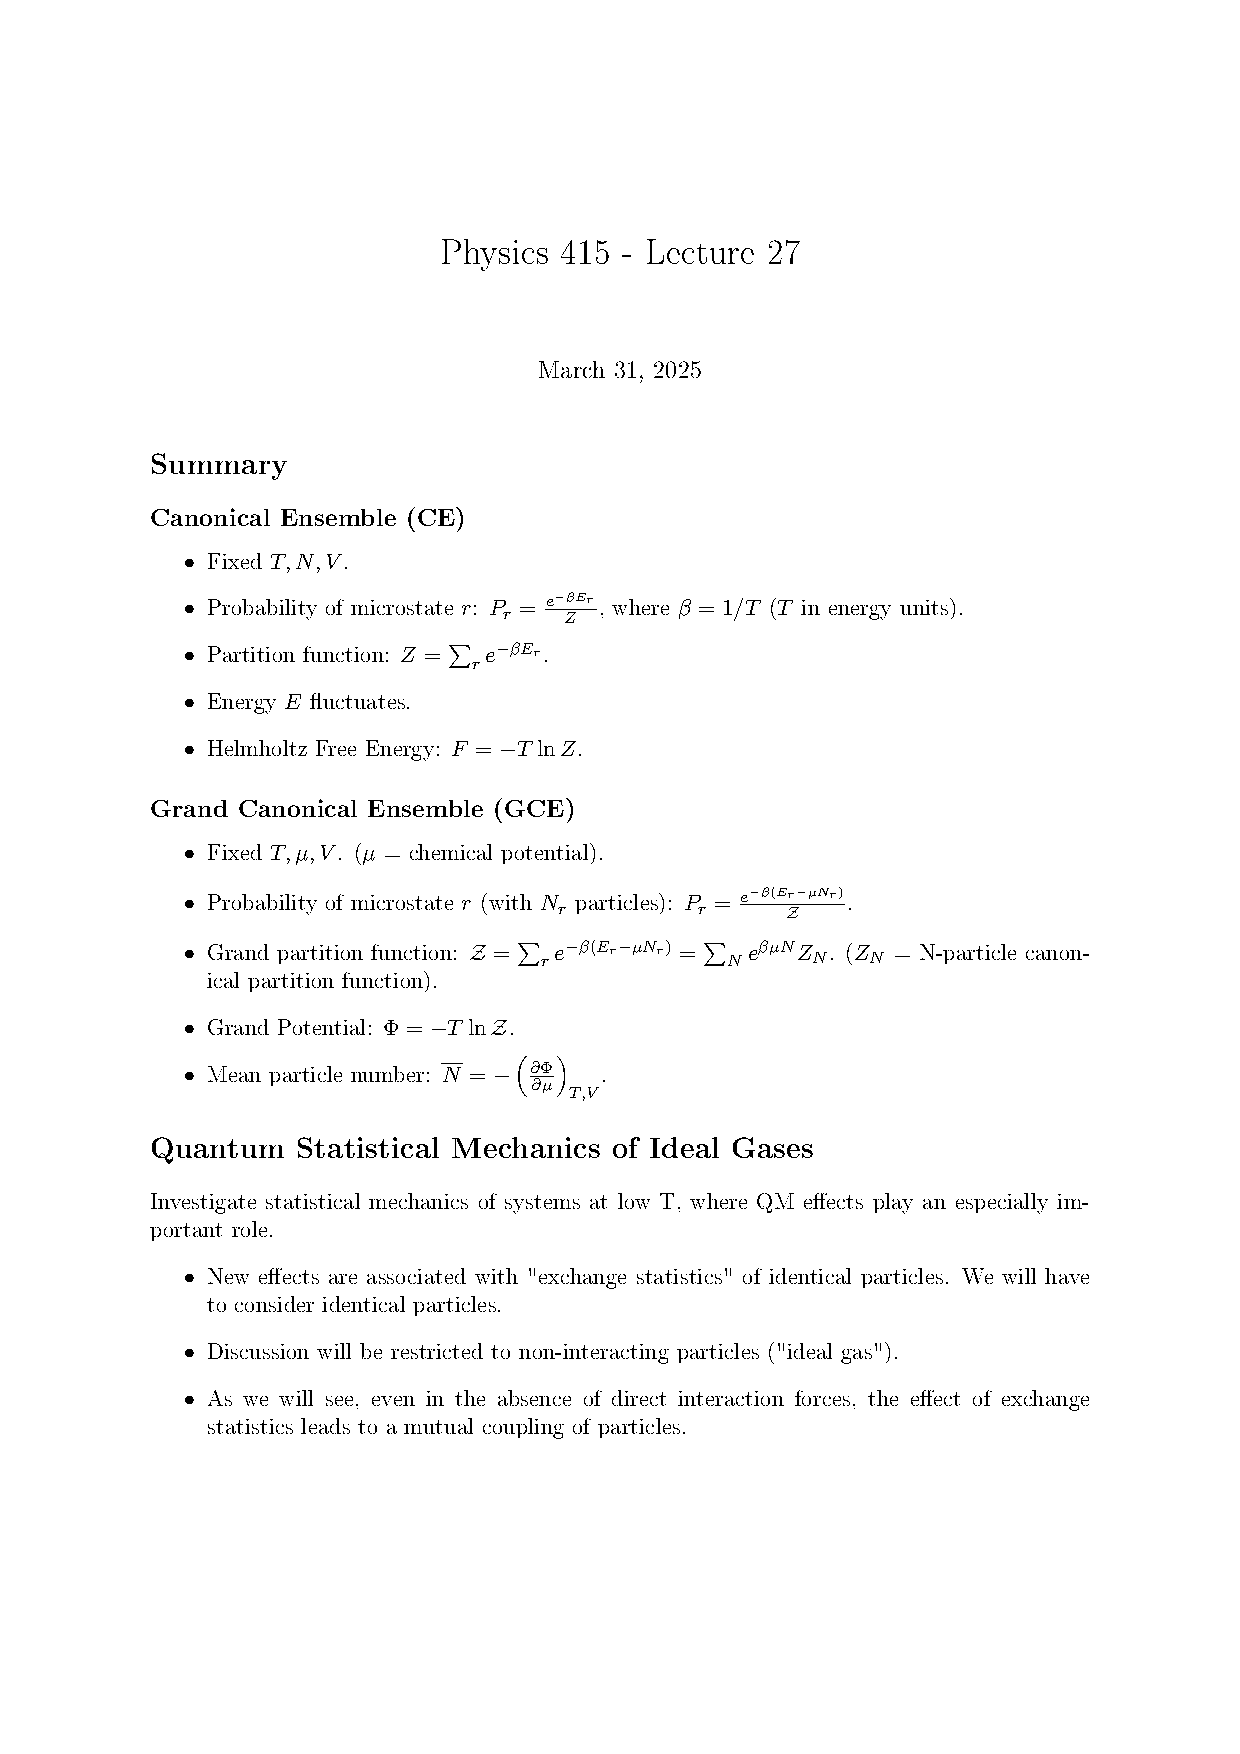
\includepdf[pages=-]{27.pdf}
\cleardoublepage
\phantomsection
\addcontentsline{toc}{chapter}{Lecture 28}
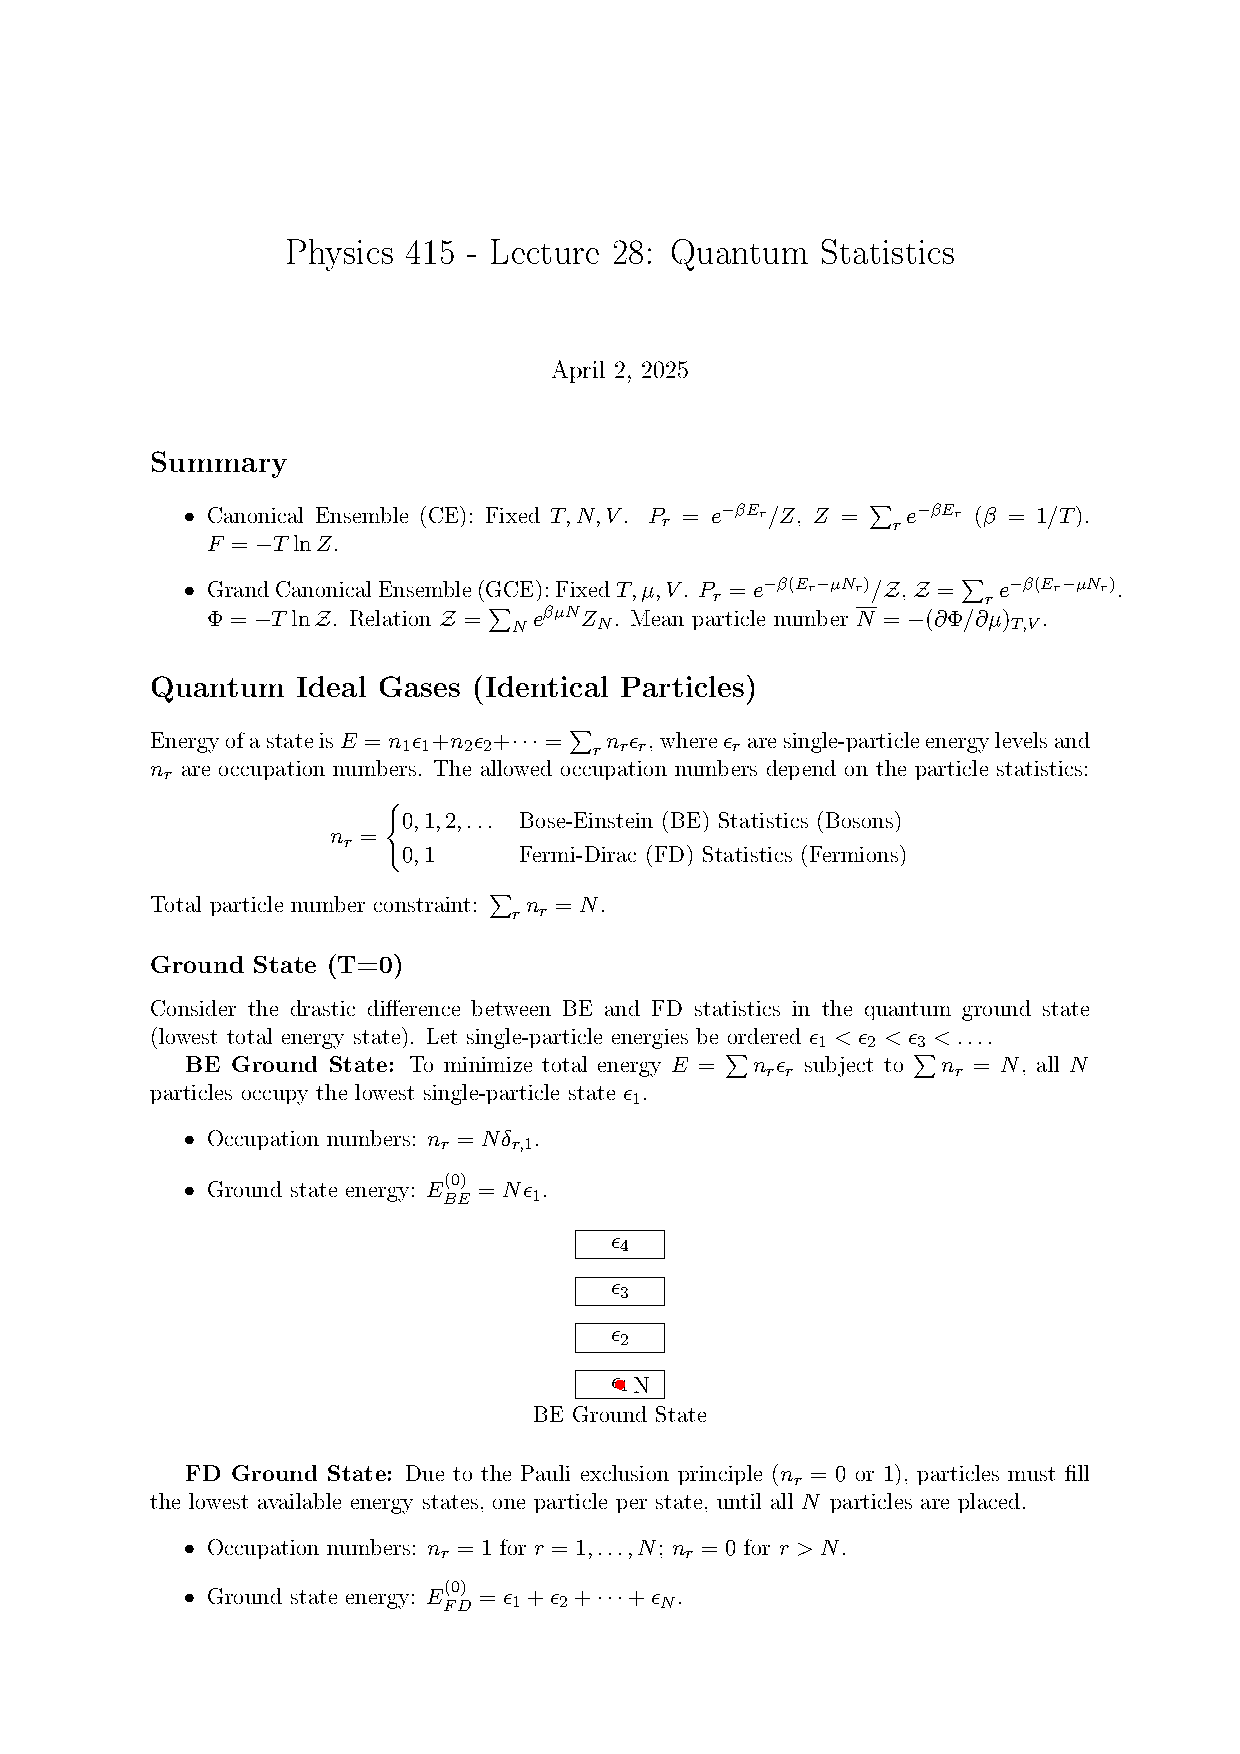
\includepdf[pages=-]{28.pdf}

% Skip 29.pdf
\cleardoublepage

% Include files 30 through 36
\phantomsection
\addcontentsline{toc}{chapter}{Lecture 30}
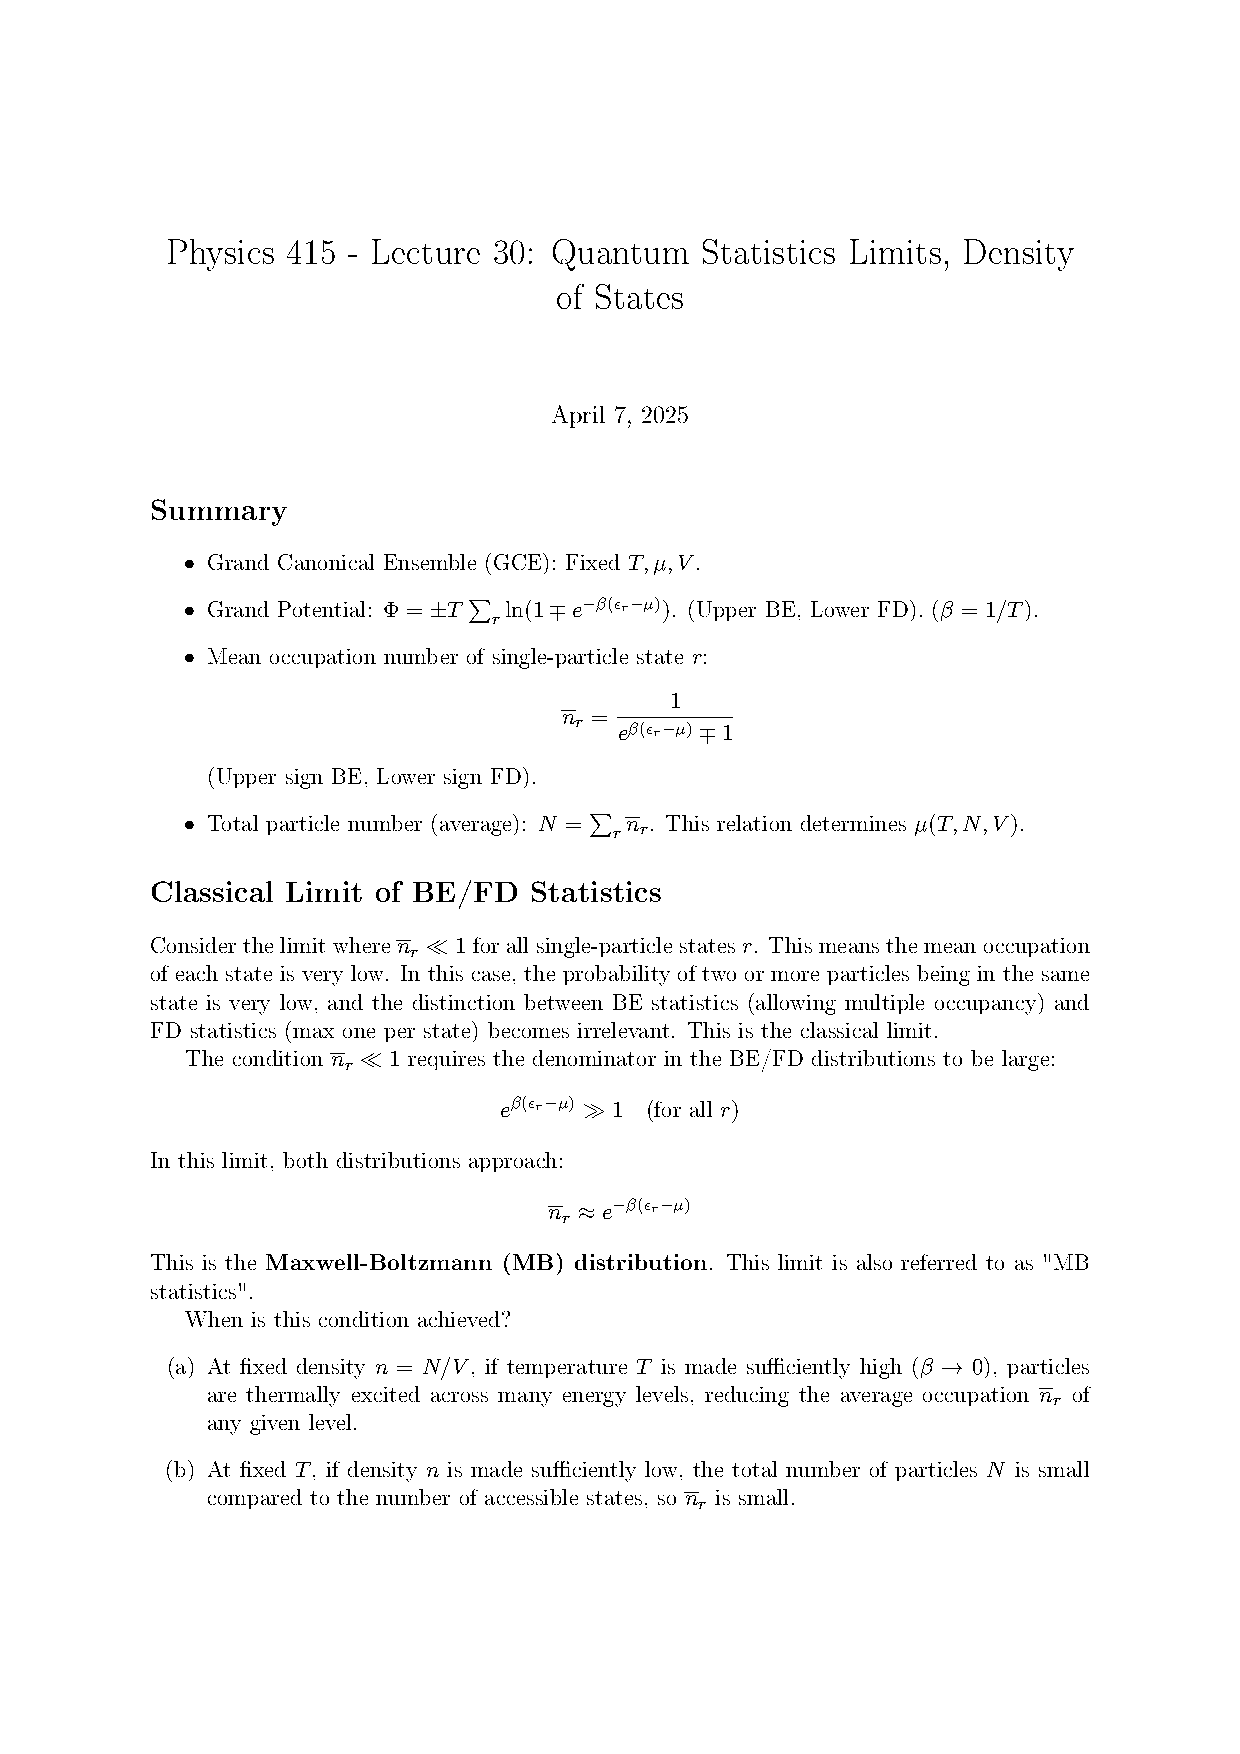
\includepdf[pages=-]{30.pdf}
\cleardoublepage
\phantomsection
\addcontentsline{toc}{chapter}{Lecture 31}
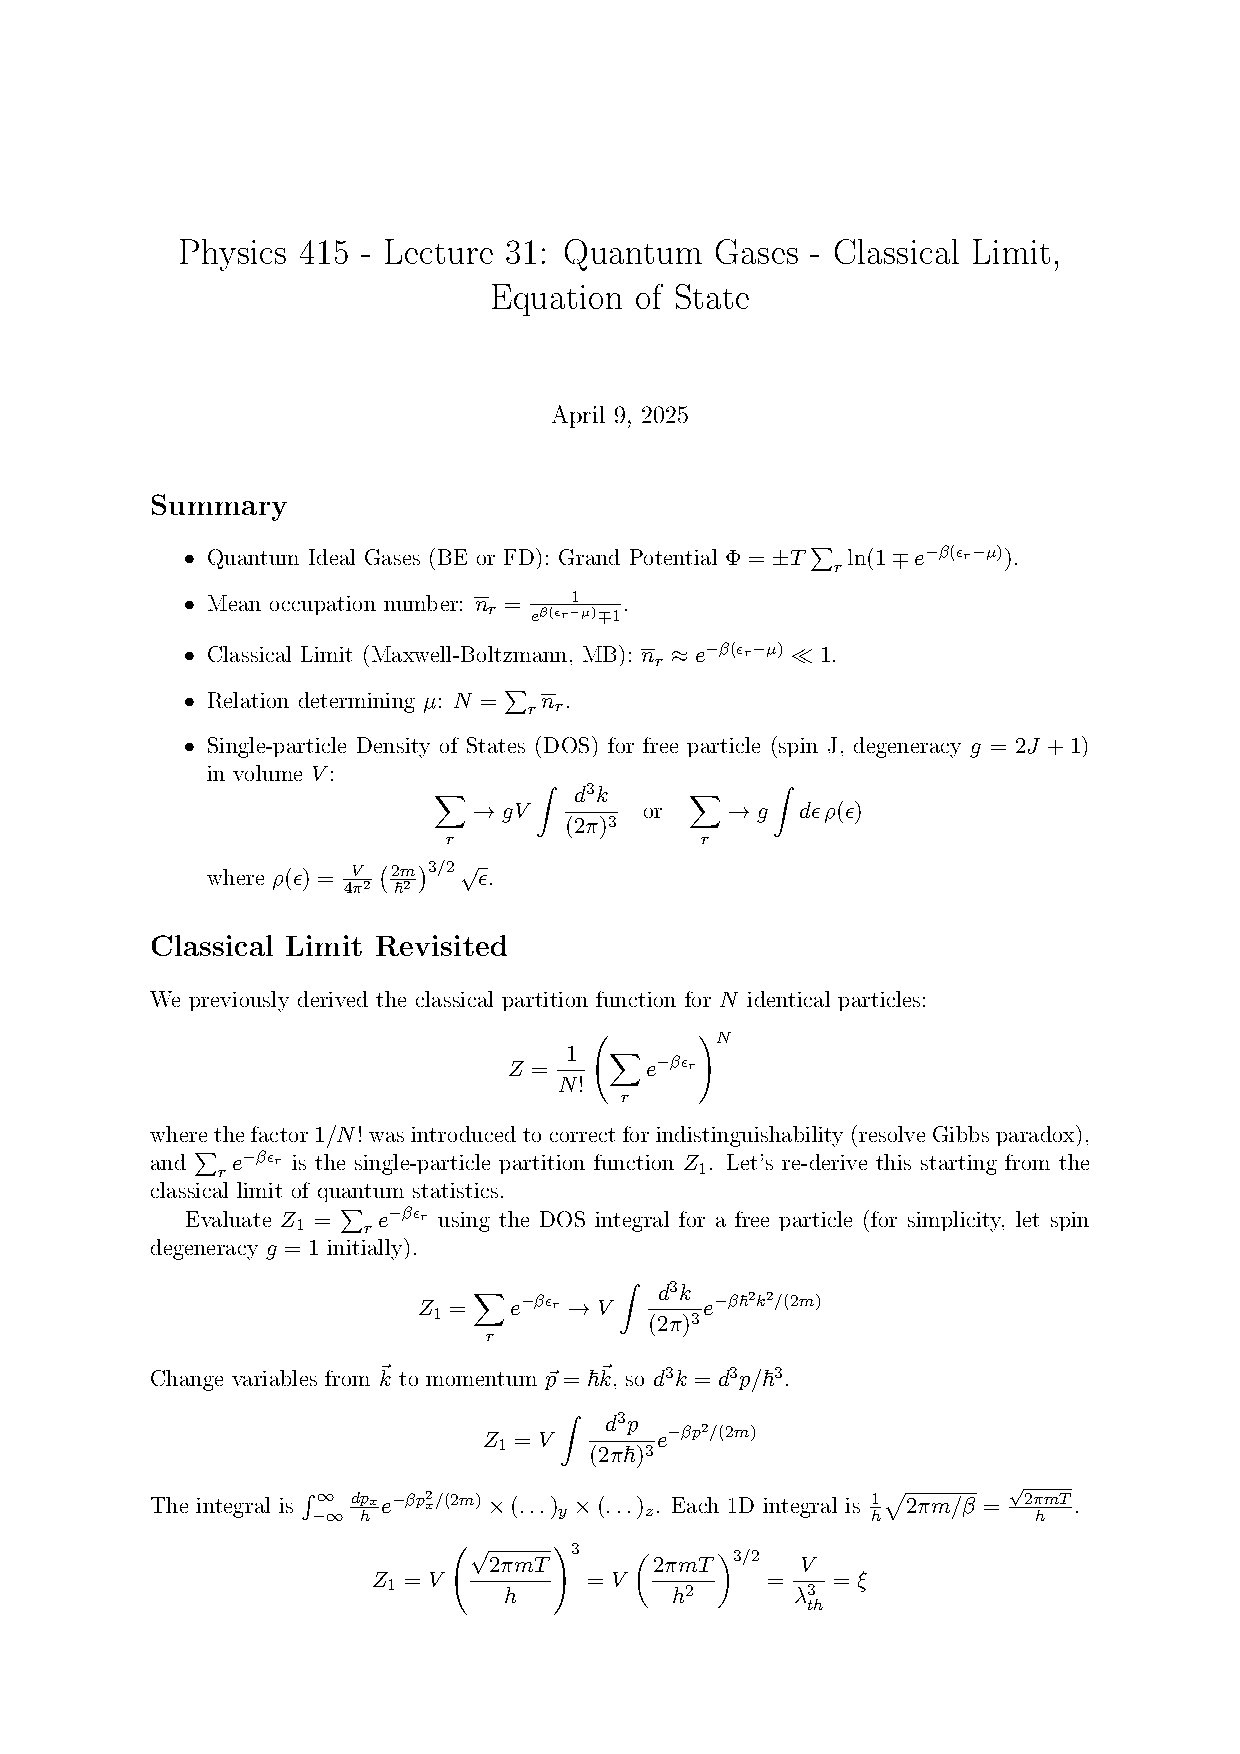
\includepdf[pages=-]{31.pdf}
\cleardoublepage
\phantomsection
\addcontentsline{toc}{chapter}{Lecture 32}
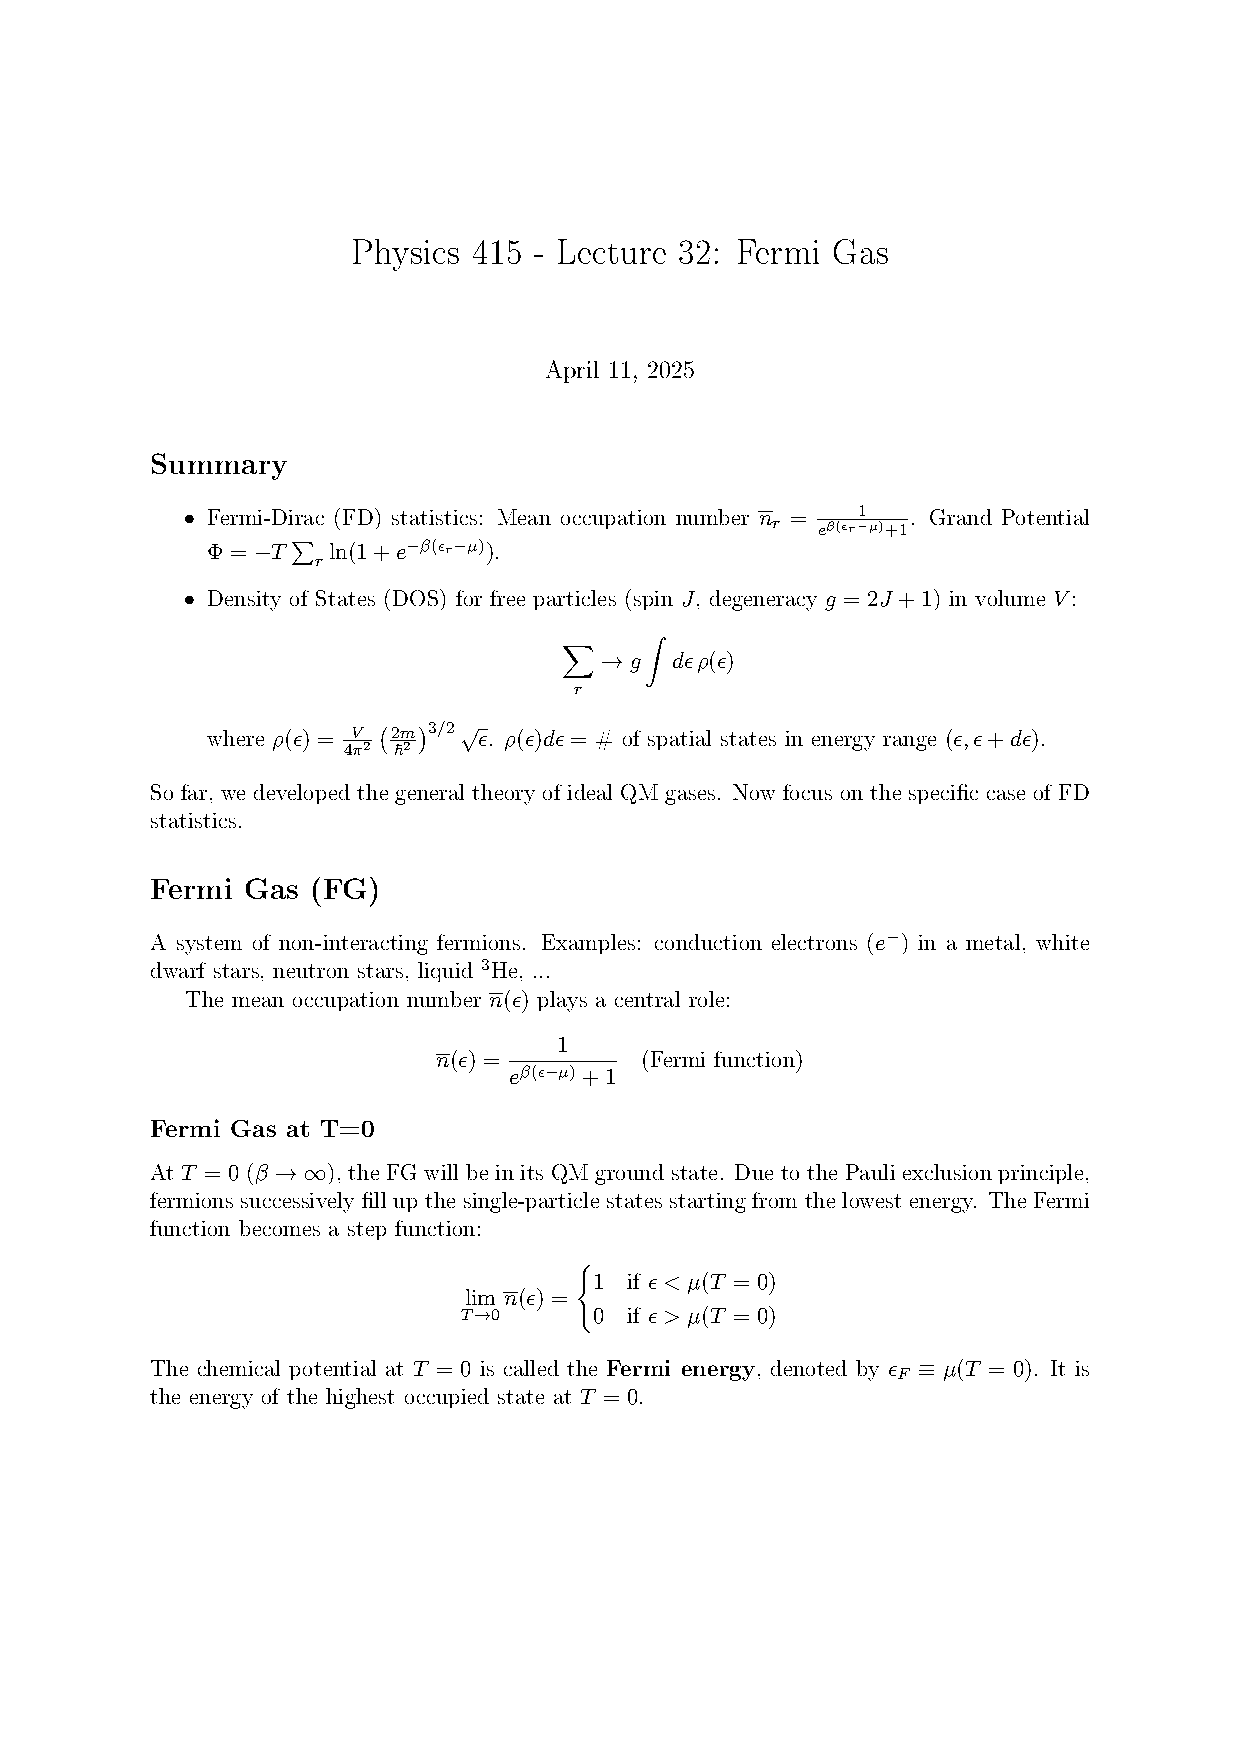
\includepdf[pages=-]{32.pdf}
\cleardoublepage
\phantomsection
\addcontentsline{toc}{chapter}{Lecture 33}
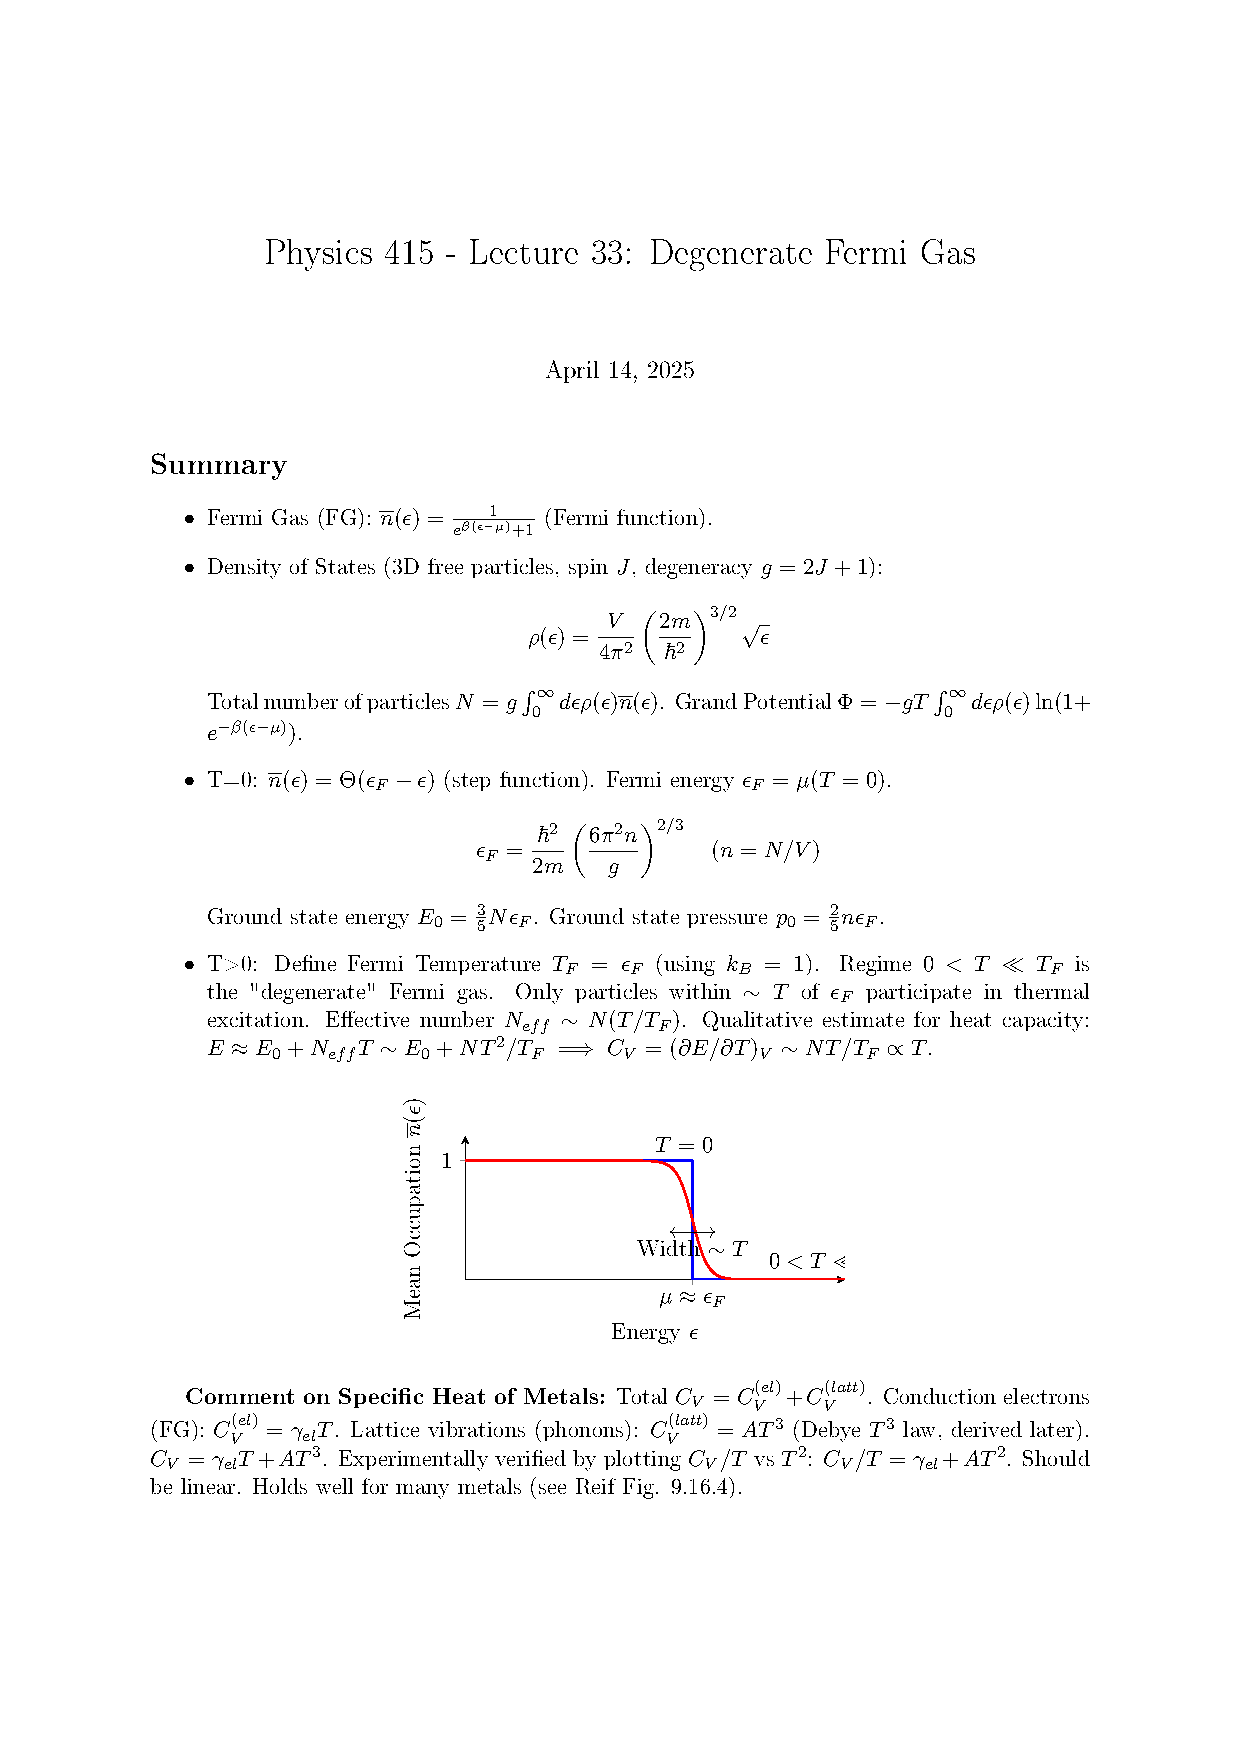
\includepdf[pages=-]{33.pdf}
\cleardoublepage
\phantomsection
\addcontentsline{toc}{chapter}{Lecture 34}
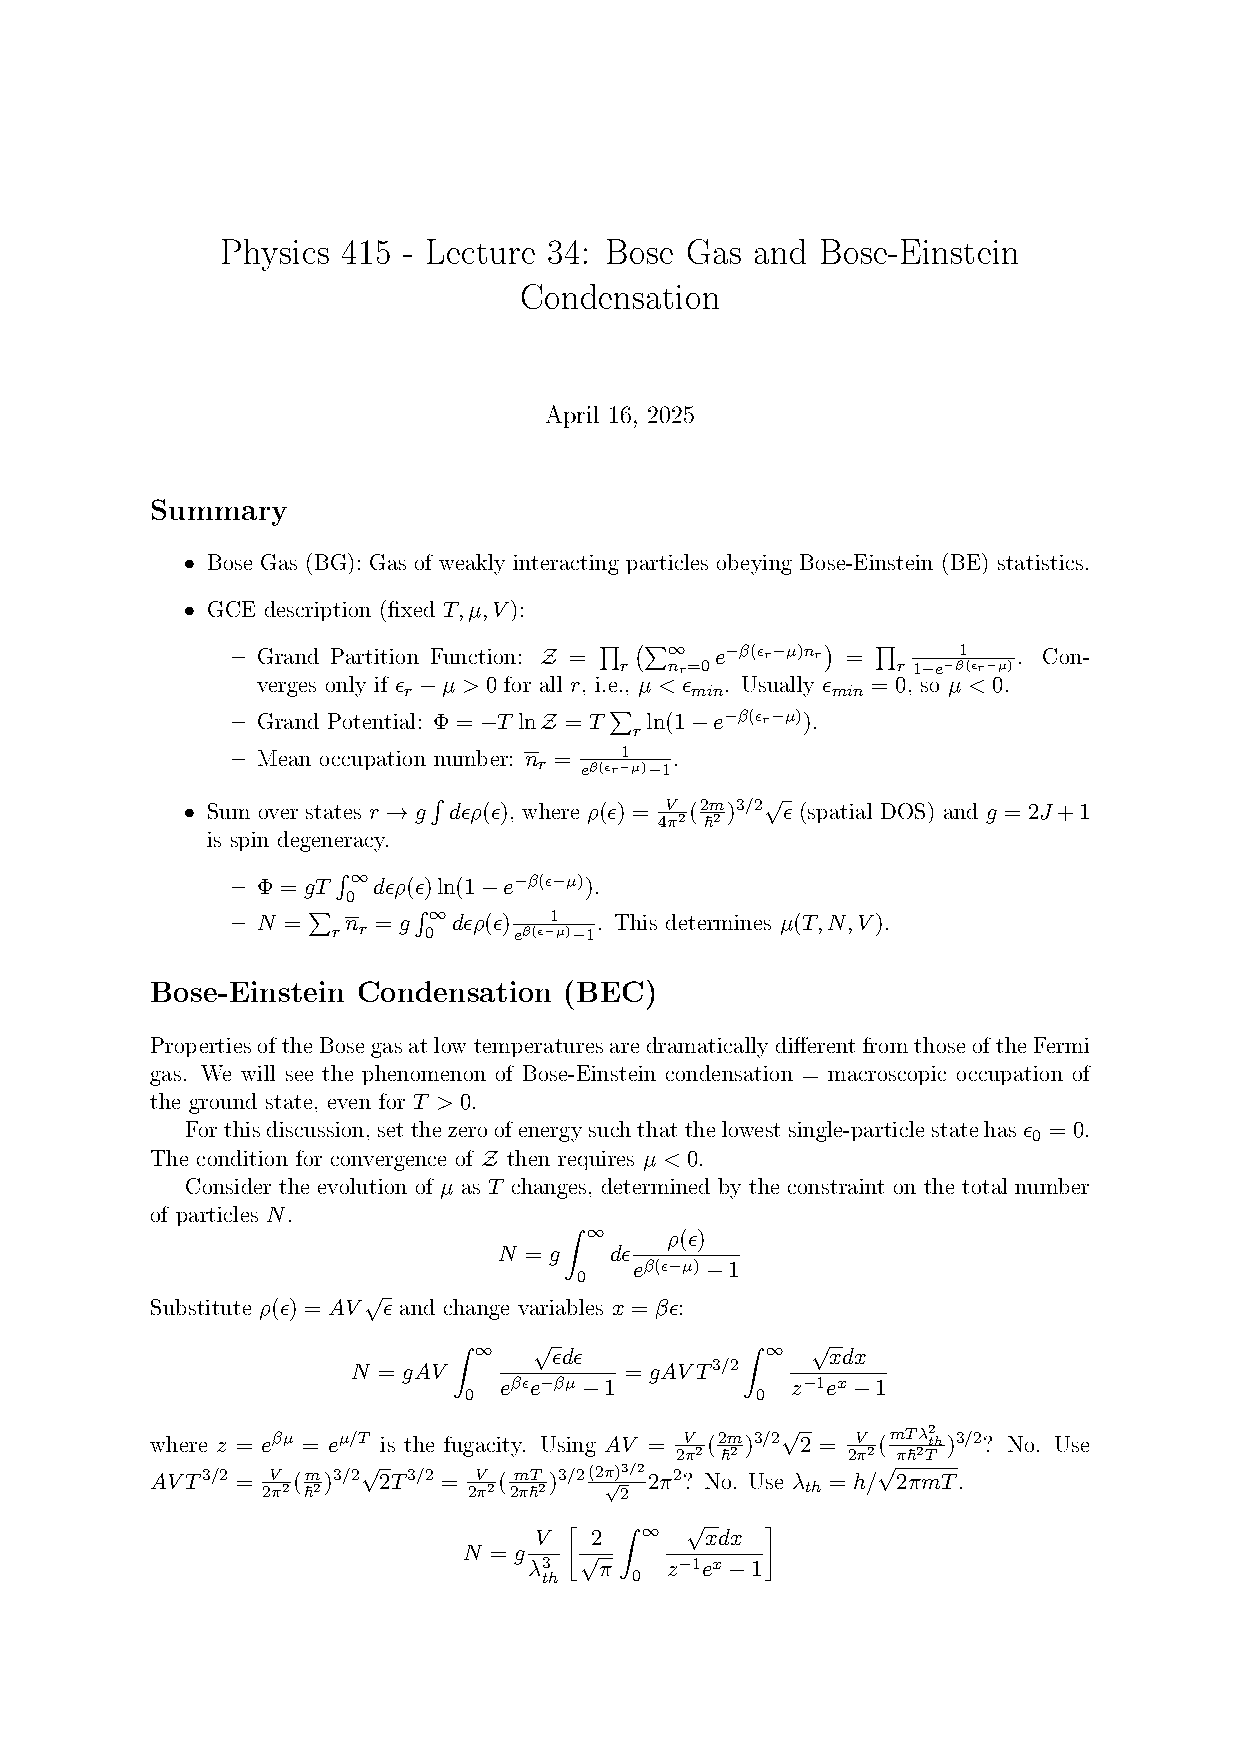
\includepdf[pages=-]{34.pdf}
\cleardoublepage
\phantomsection
\addcontentsline{toc}{chapter}{Lecture 35}
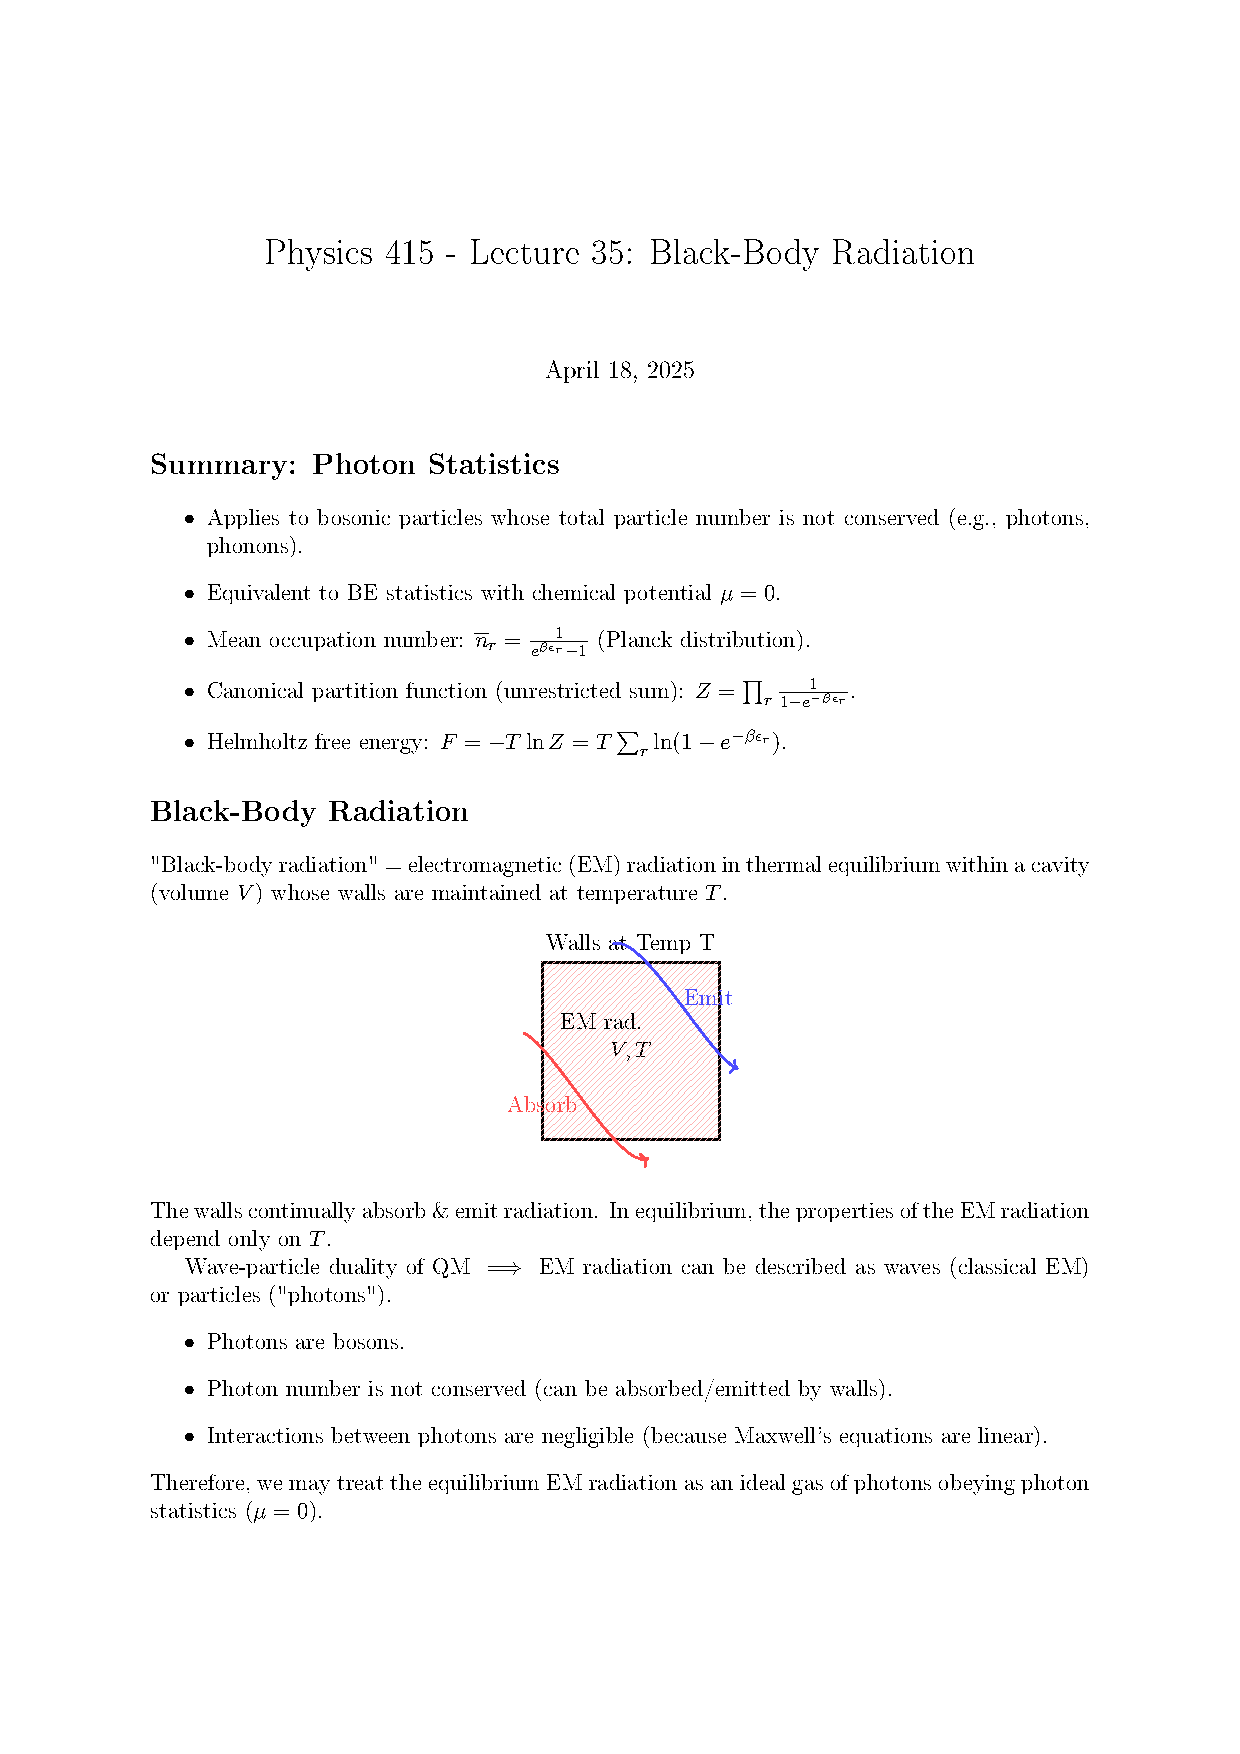
\includepdf[pages=-]{35.pdf}
\cleardoublepage
\phantomsection
\addcontentsline{toc}{chapter}{Lecture 36}
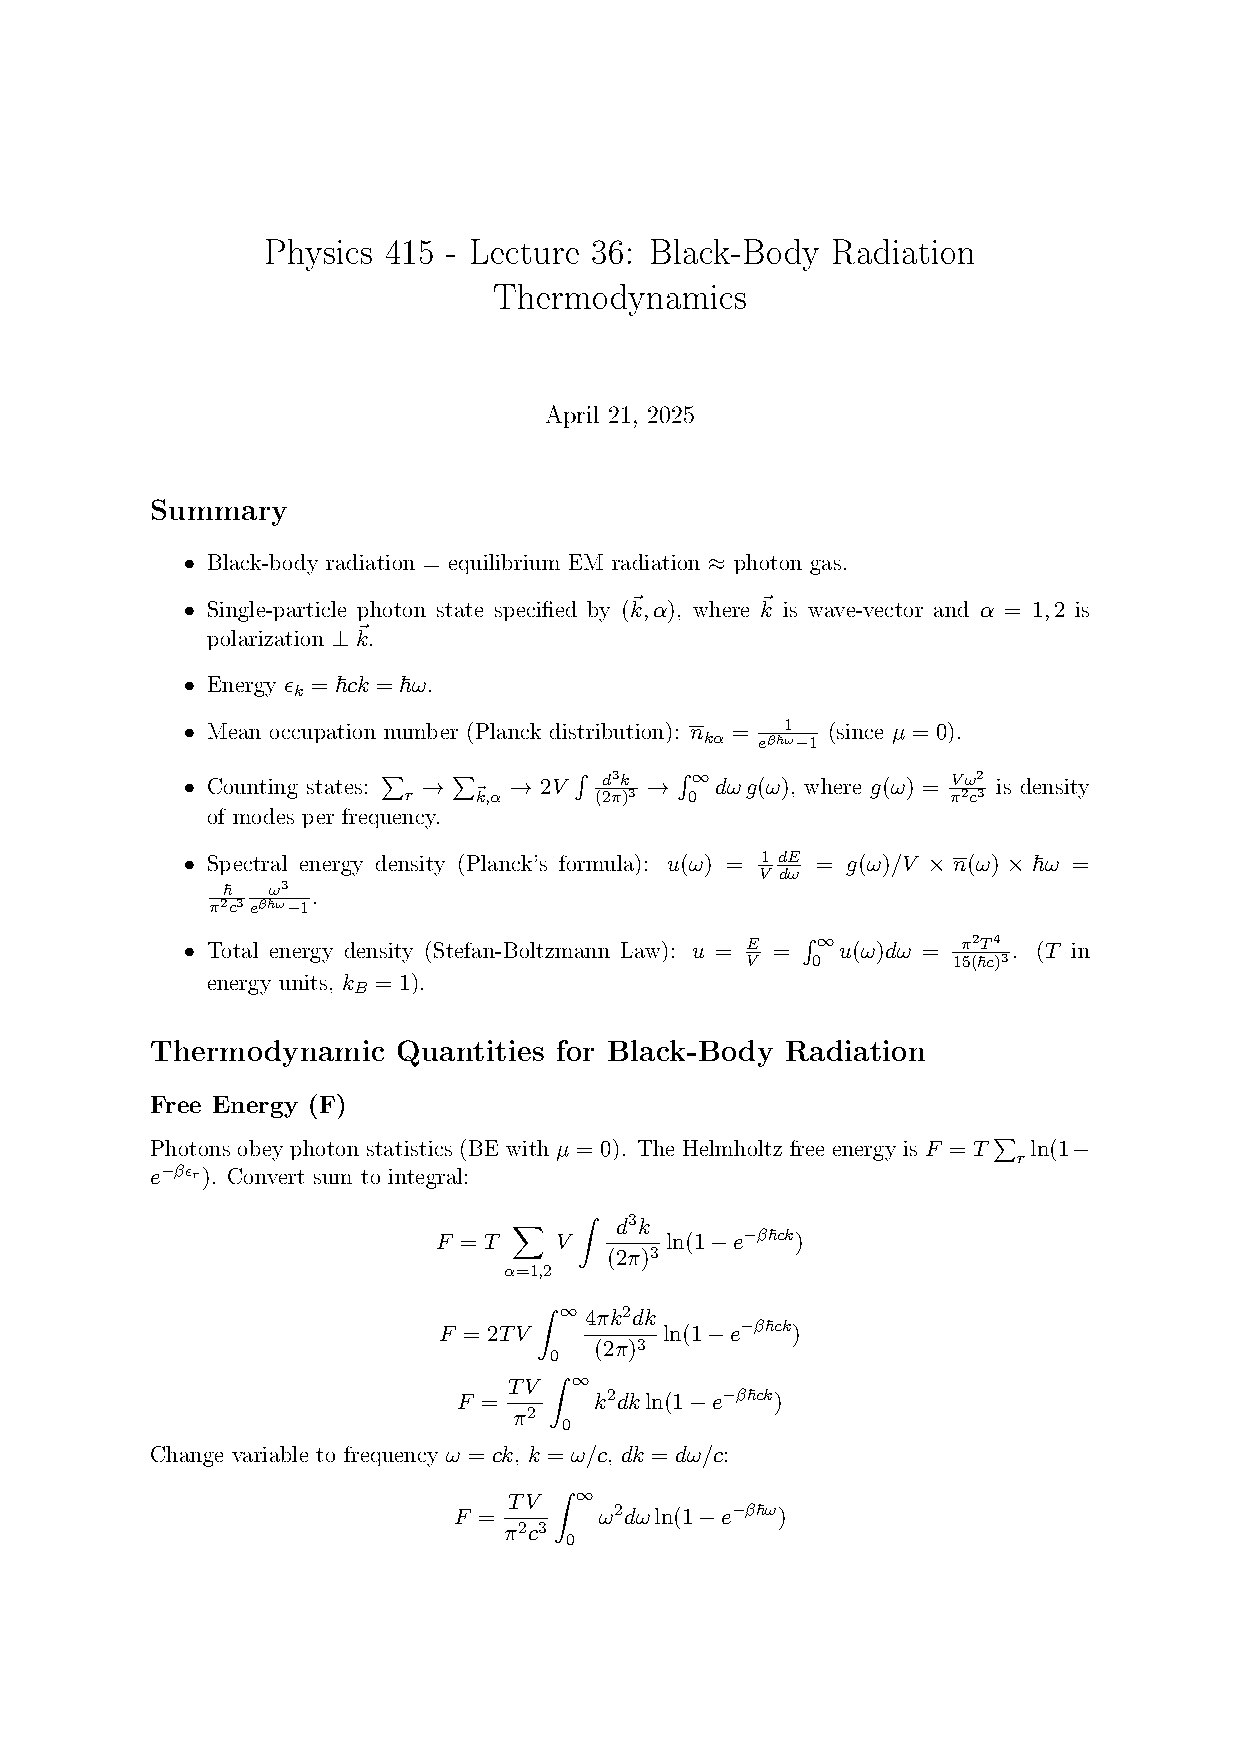
\includepdf[pages=-]{36.pdf}

\end{document}